%PDF DI RIFERIMENTO: 04_Modelli di Dominio.pdf, Statecharts.pdf

\chapter{Requirement Specification}
    \section{Obiettivo}
        I requisiti che sono stati riorganizzati nella fase di analisi sono formalizzati in diagrammi (diagramma di classe, diagramma di sequenza, diagramma degli stati) attraverso l'uso di linguaggi di modellazione come UML. \\
        Per individuare il modello ad oggetti per questo dominio, si è scelto di impiegare l'euristica "Three-Object-Type" perché permette di costruire un modello più flessibile e facile da modificare.

    \section{Class Diagram}
        Il Class Diagram individua quali sono le entità coinvolte all'interno del nostro dominio e le relazioni che tra esse sussistono.\\
        In particolare, il modello concettuale basato sull'analisi dei requisiti permetterà di creare un modello efficace per la gestione delle aste.\\
        
        \subsection{Class Diagram del dominio del problema}
            % Class Diagram costruito con StarUML
            \begin{figure}[htbp!]
                \centering
                    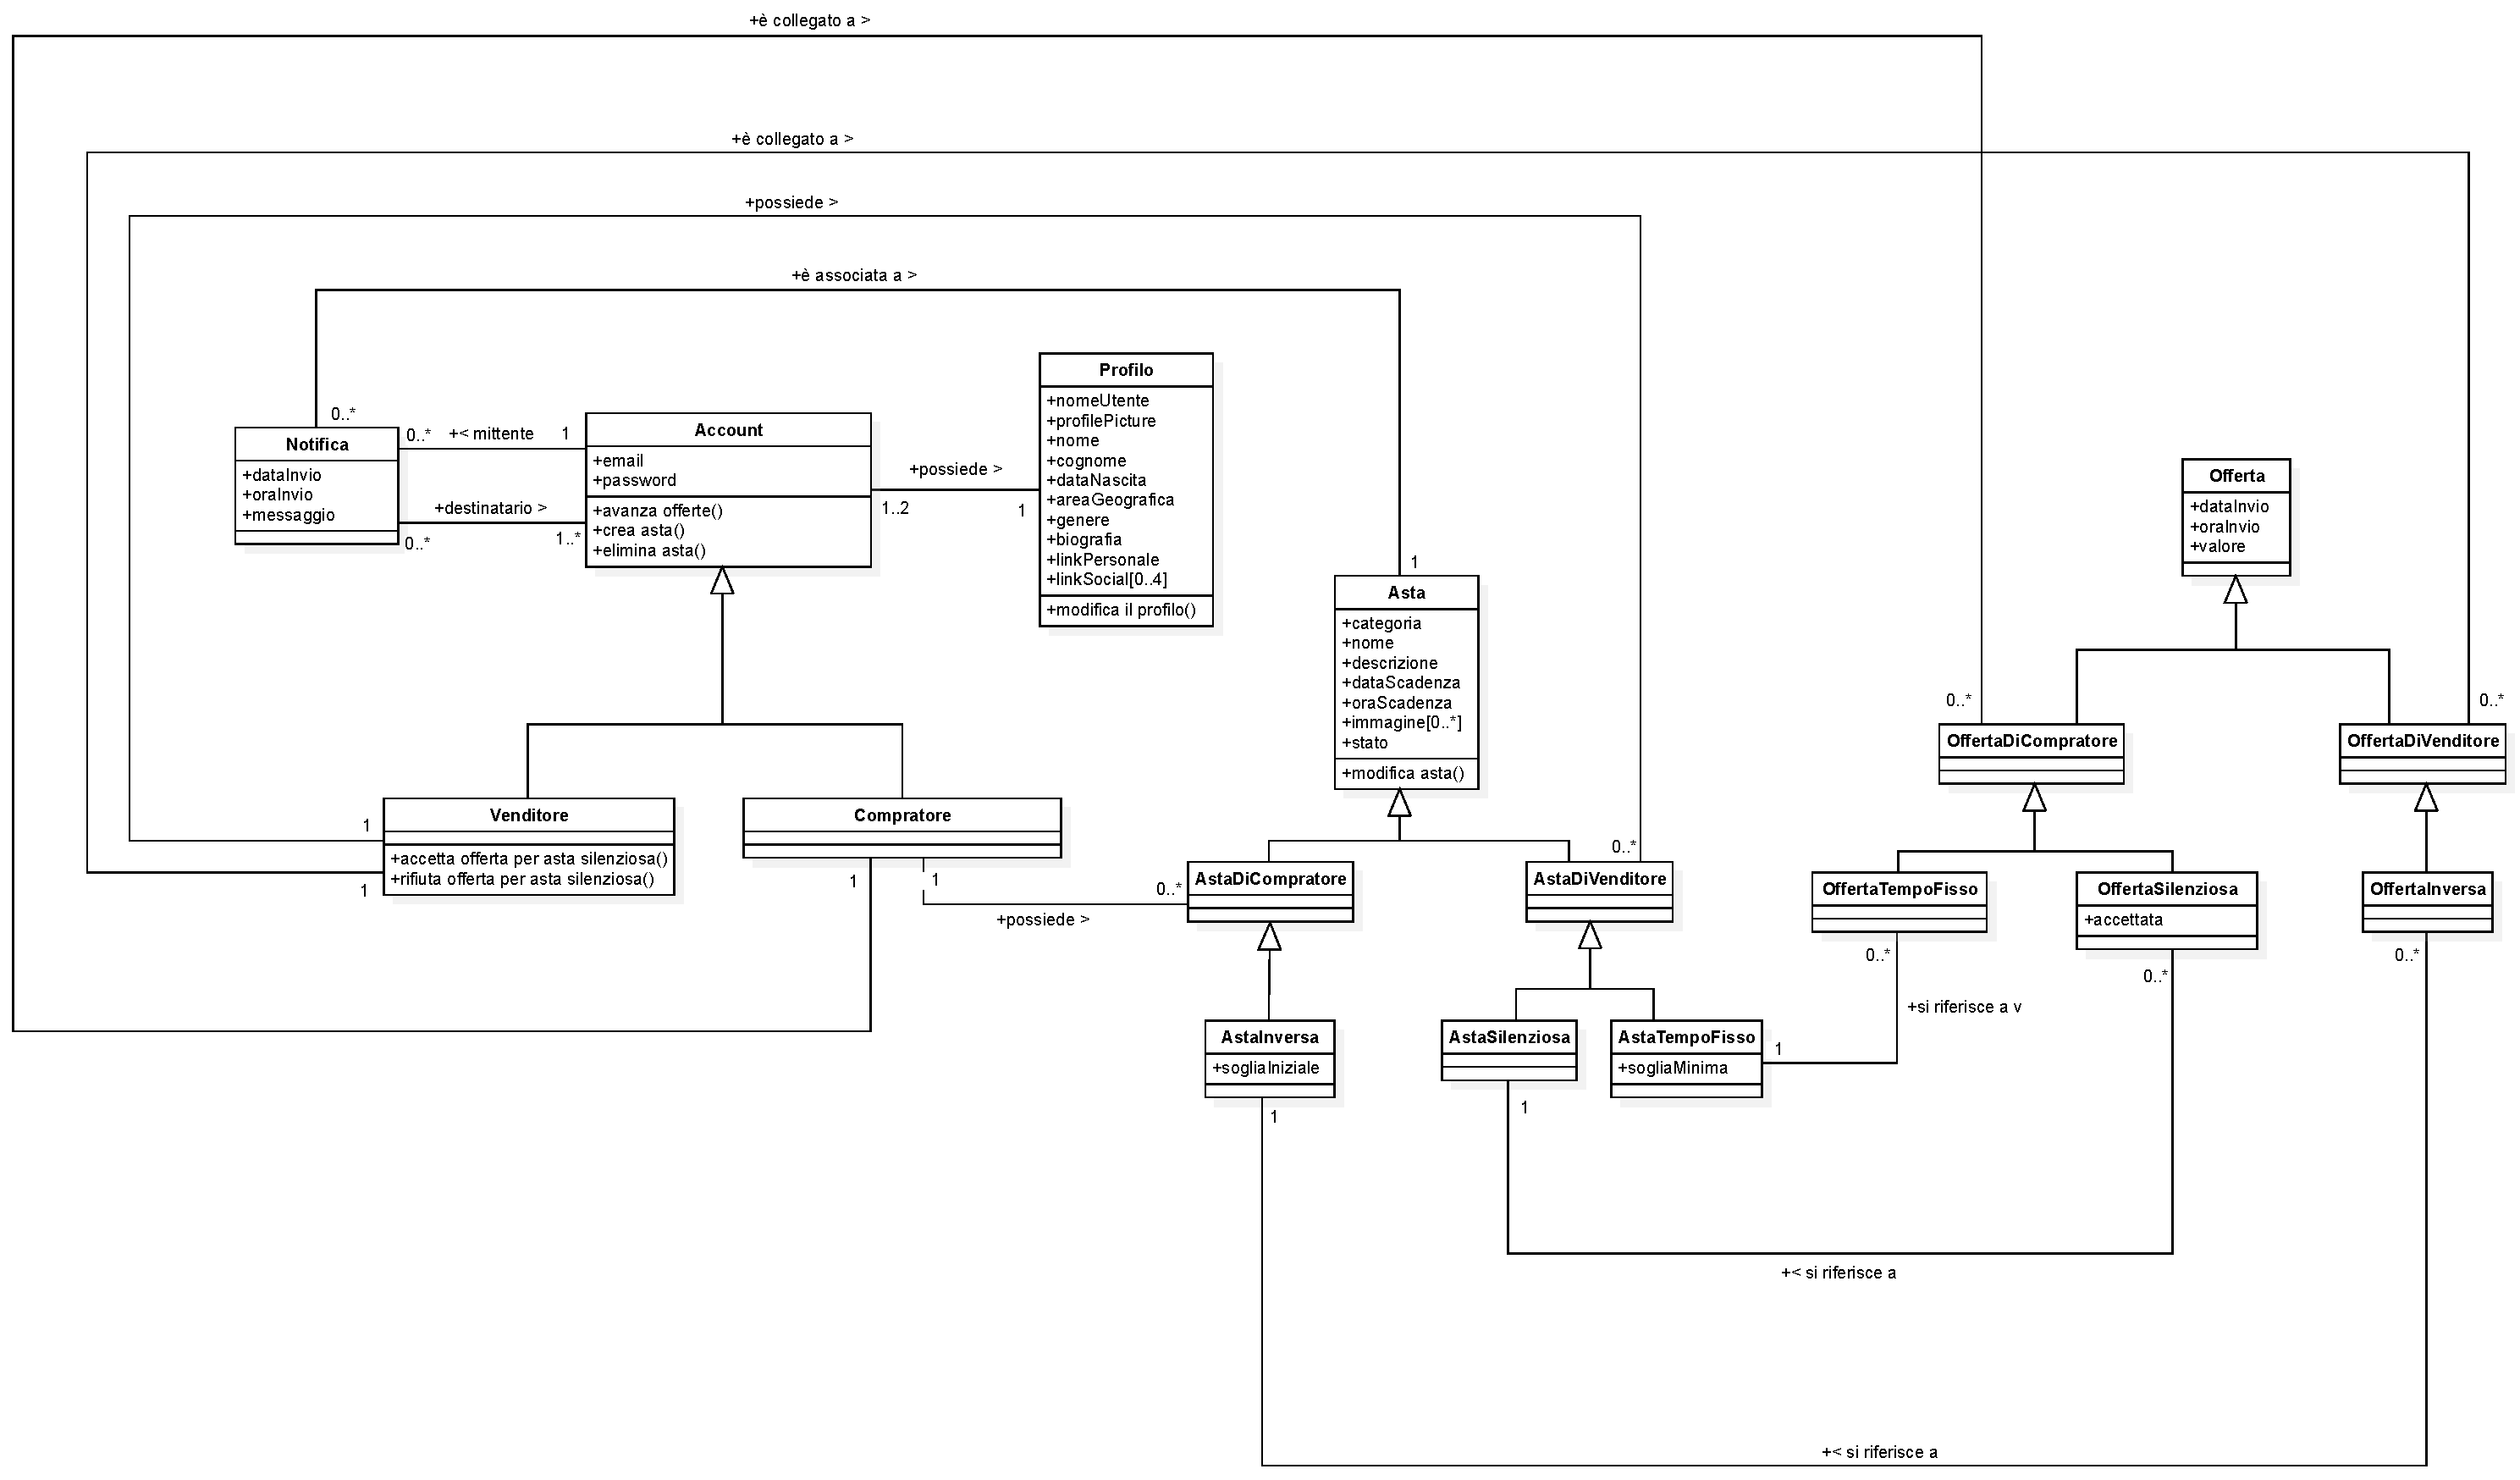
\includegraphics[width=1\linewidth]{Immagini/Diagrammi/Class Diagram/Analisi/ClassDiagramDominio.pdf}
                \caption{Class Diagram del dominio del problema}
                \label{fig:Class Diagram del dominio del problema}
            \end{figure}
            
        \subsection{Class Diagram per casi d'uso}
            In questa sezione verranno mostrati i diagrammi secondo l'euristica "Three-Object-Type" per ogni caso d'uso. Le classi possono essere di tipo "Boundary", "Control" e "Entity".
        
            \begin{figure}[htbp!]
                \centering
                    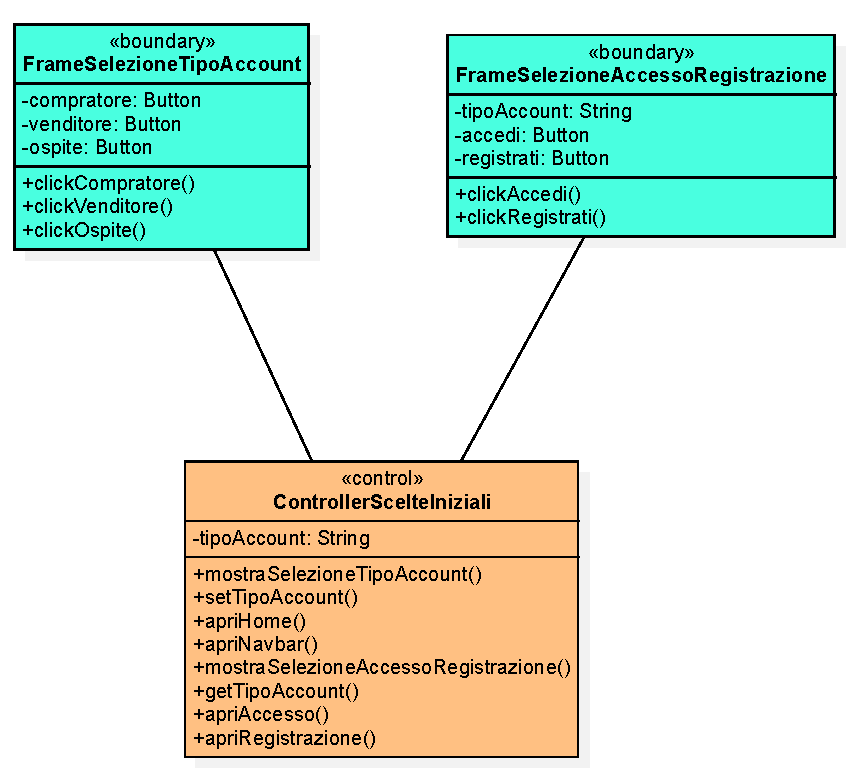
\includegraphics[width=1\linewidth]{Immagini/Diagrammi/Class Diagram/Analisi/Utente che non ha effettuato l'accesso/ScelteIniziali.pdf}
                \caption{Scelta del tipo di account}
            \end{figure}
            
            \begin{figure}[htbp!]
                \centering
                    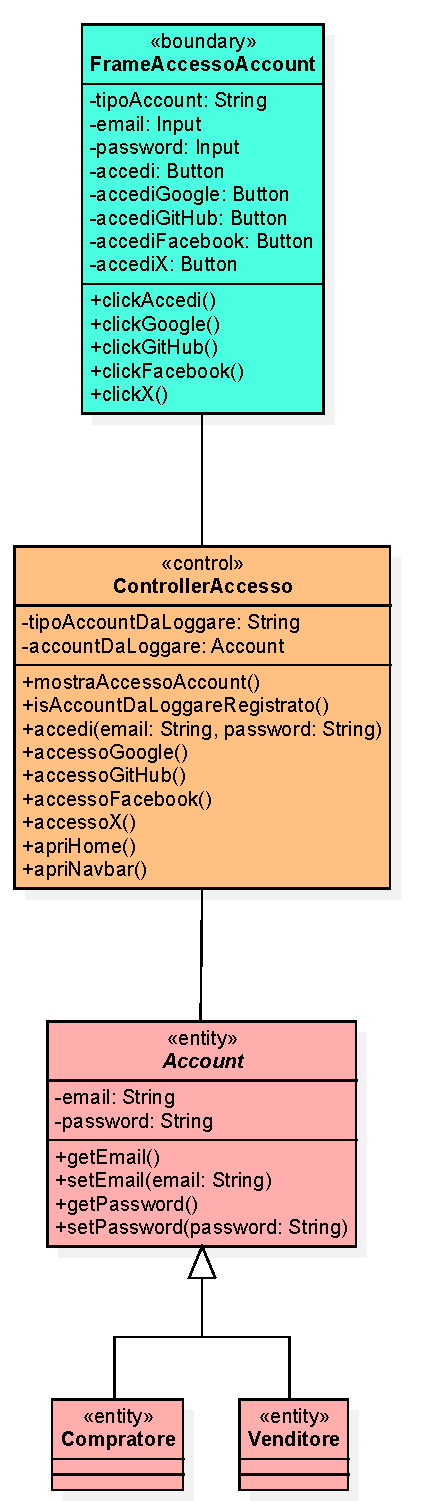
\includegraphics[width=0.35\linewidth]{Immagini/Diagrammi/Class Diagram/Analisi/Utente che non ha effettuato l'accesso/Accesso.pdf}
                \caption{Accesso}
            \end{figure}
            
            \begin{figure}[htbp!]
                \centering
                    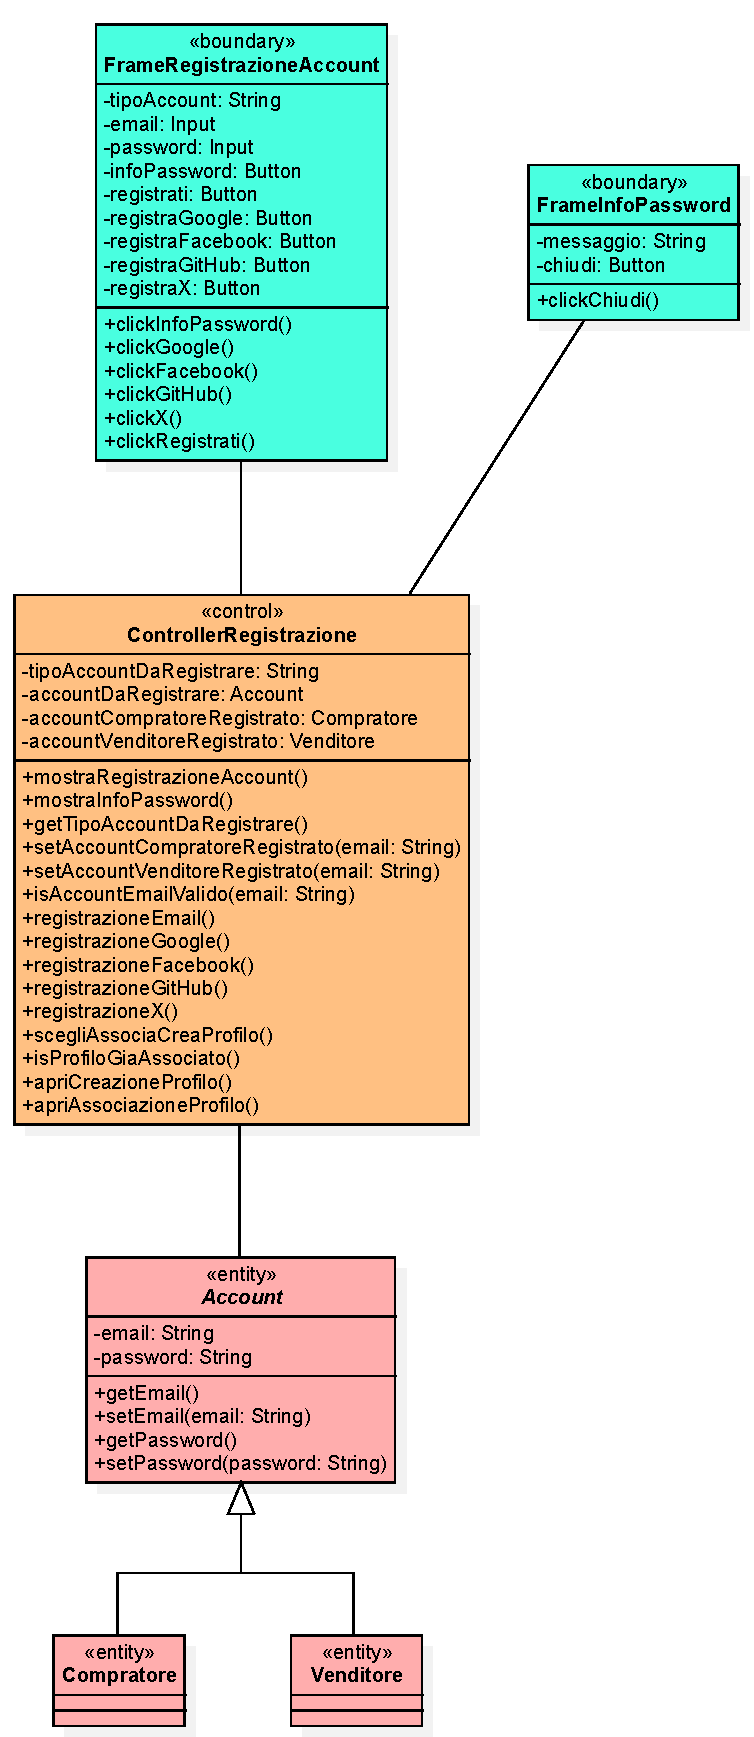
\includegraphics[width=0.55\linewidth]{Immagini/Diagrammi/Class Diagram/Analisi/Utente che non ha effettuato l'accesso/Registrazione.pdf}
                \caption{Registrazione}
            \end{figure}
            
            \begin{figure}[htbp!]
                \centering
                    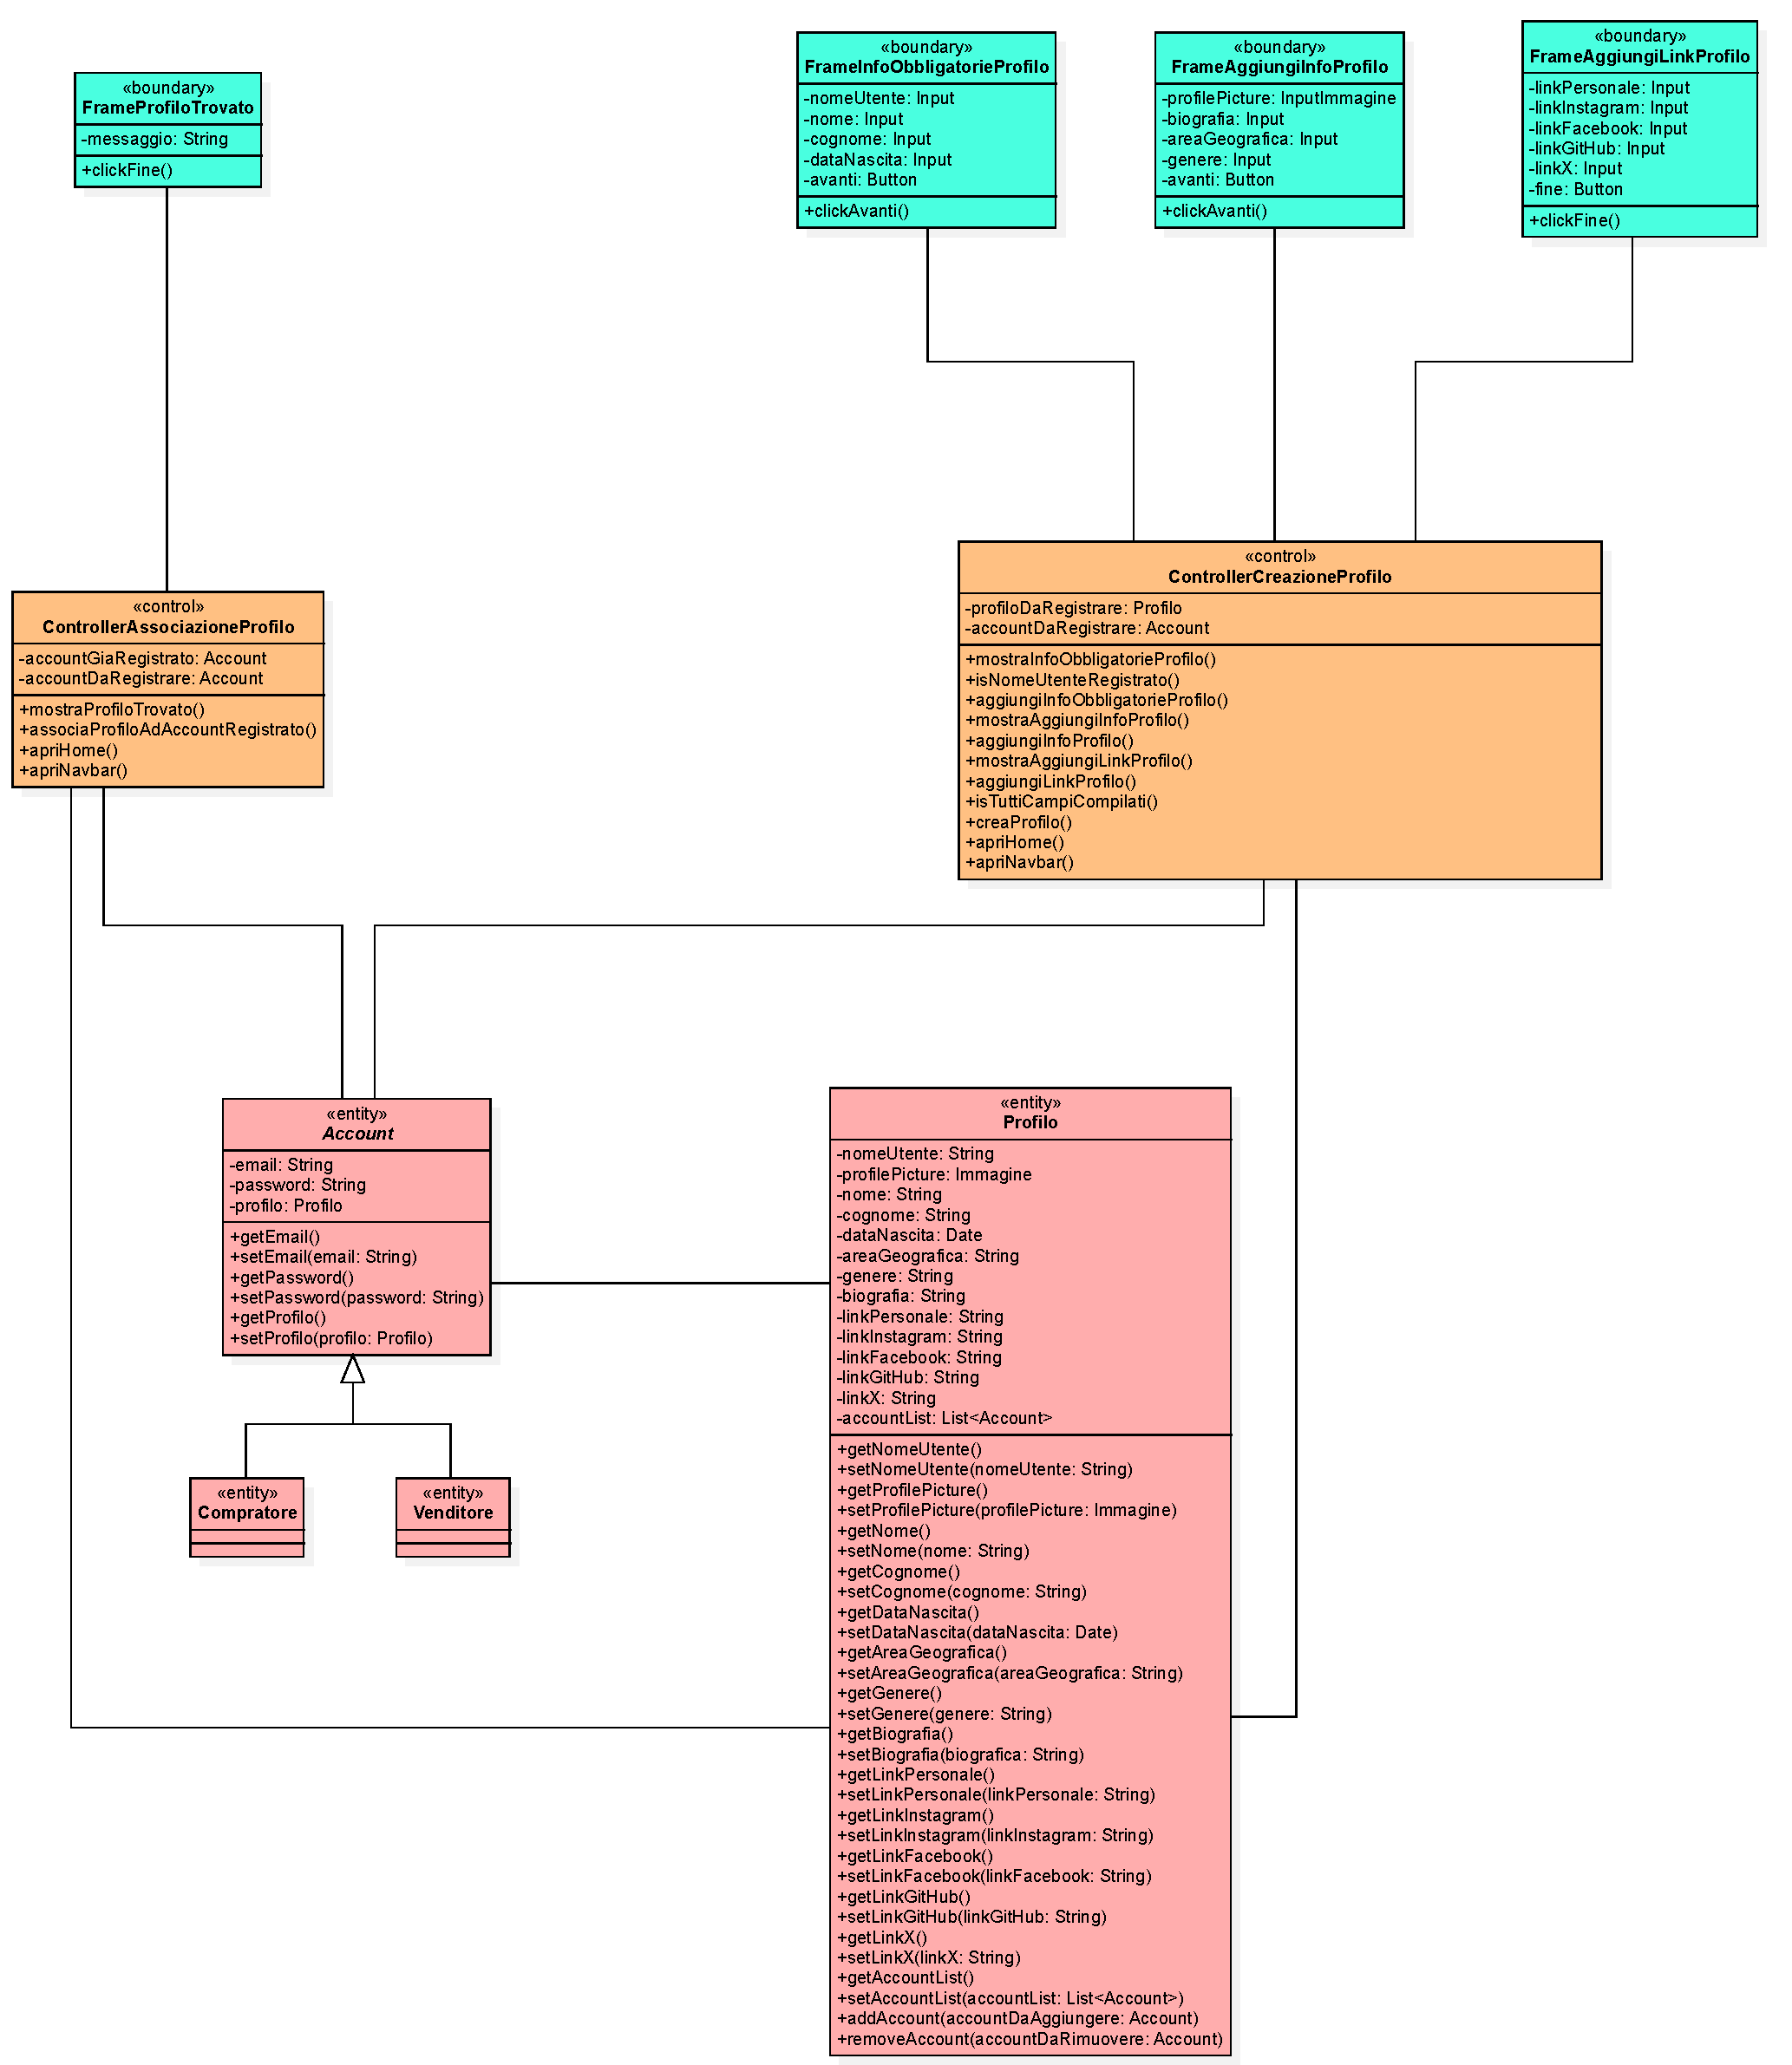
\includegraphics[width=1\linewidth]{Immagini/Diagrammi/Class Diagram/Analisi/Utente che non ha effettuato l'accesso/CreazioneProfilo.pdf}
                \caption{Creazione del profilo}
            \end{figure}
            
            \begin{figure}[htbp!]
                \centering
                    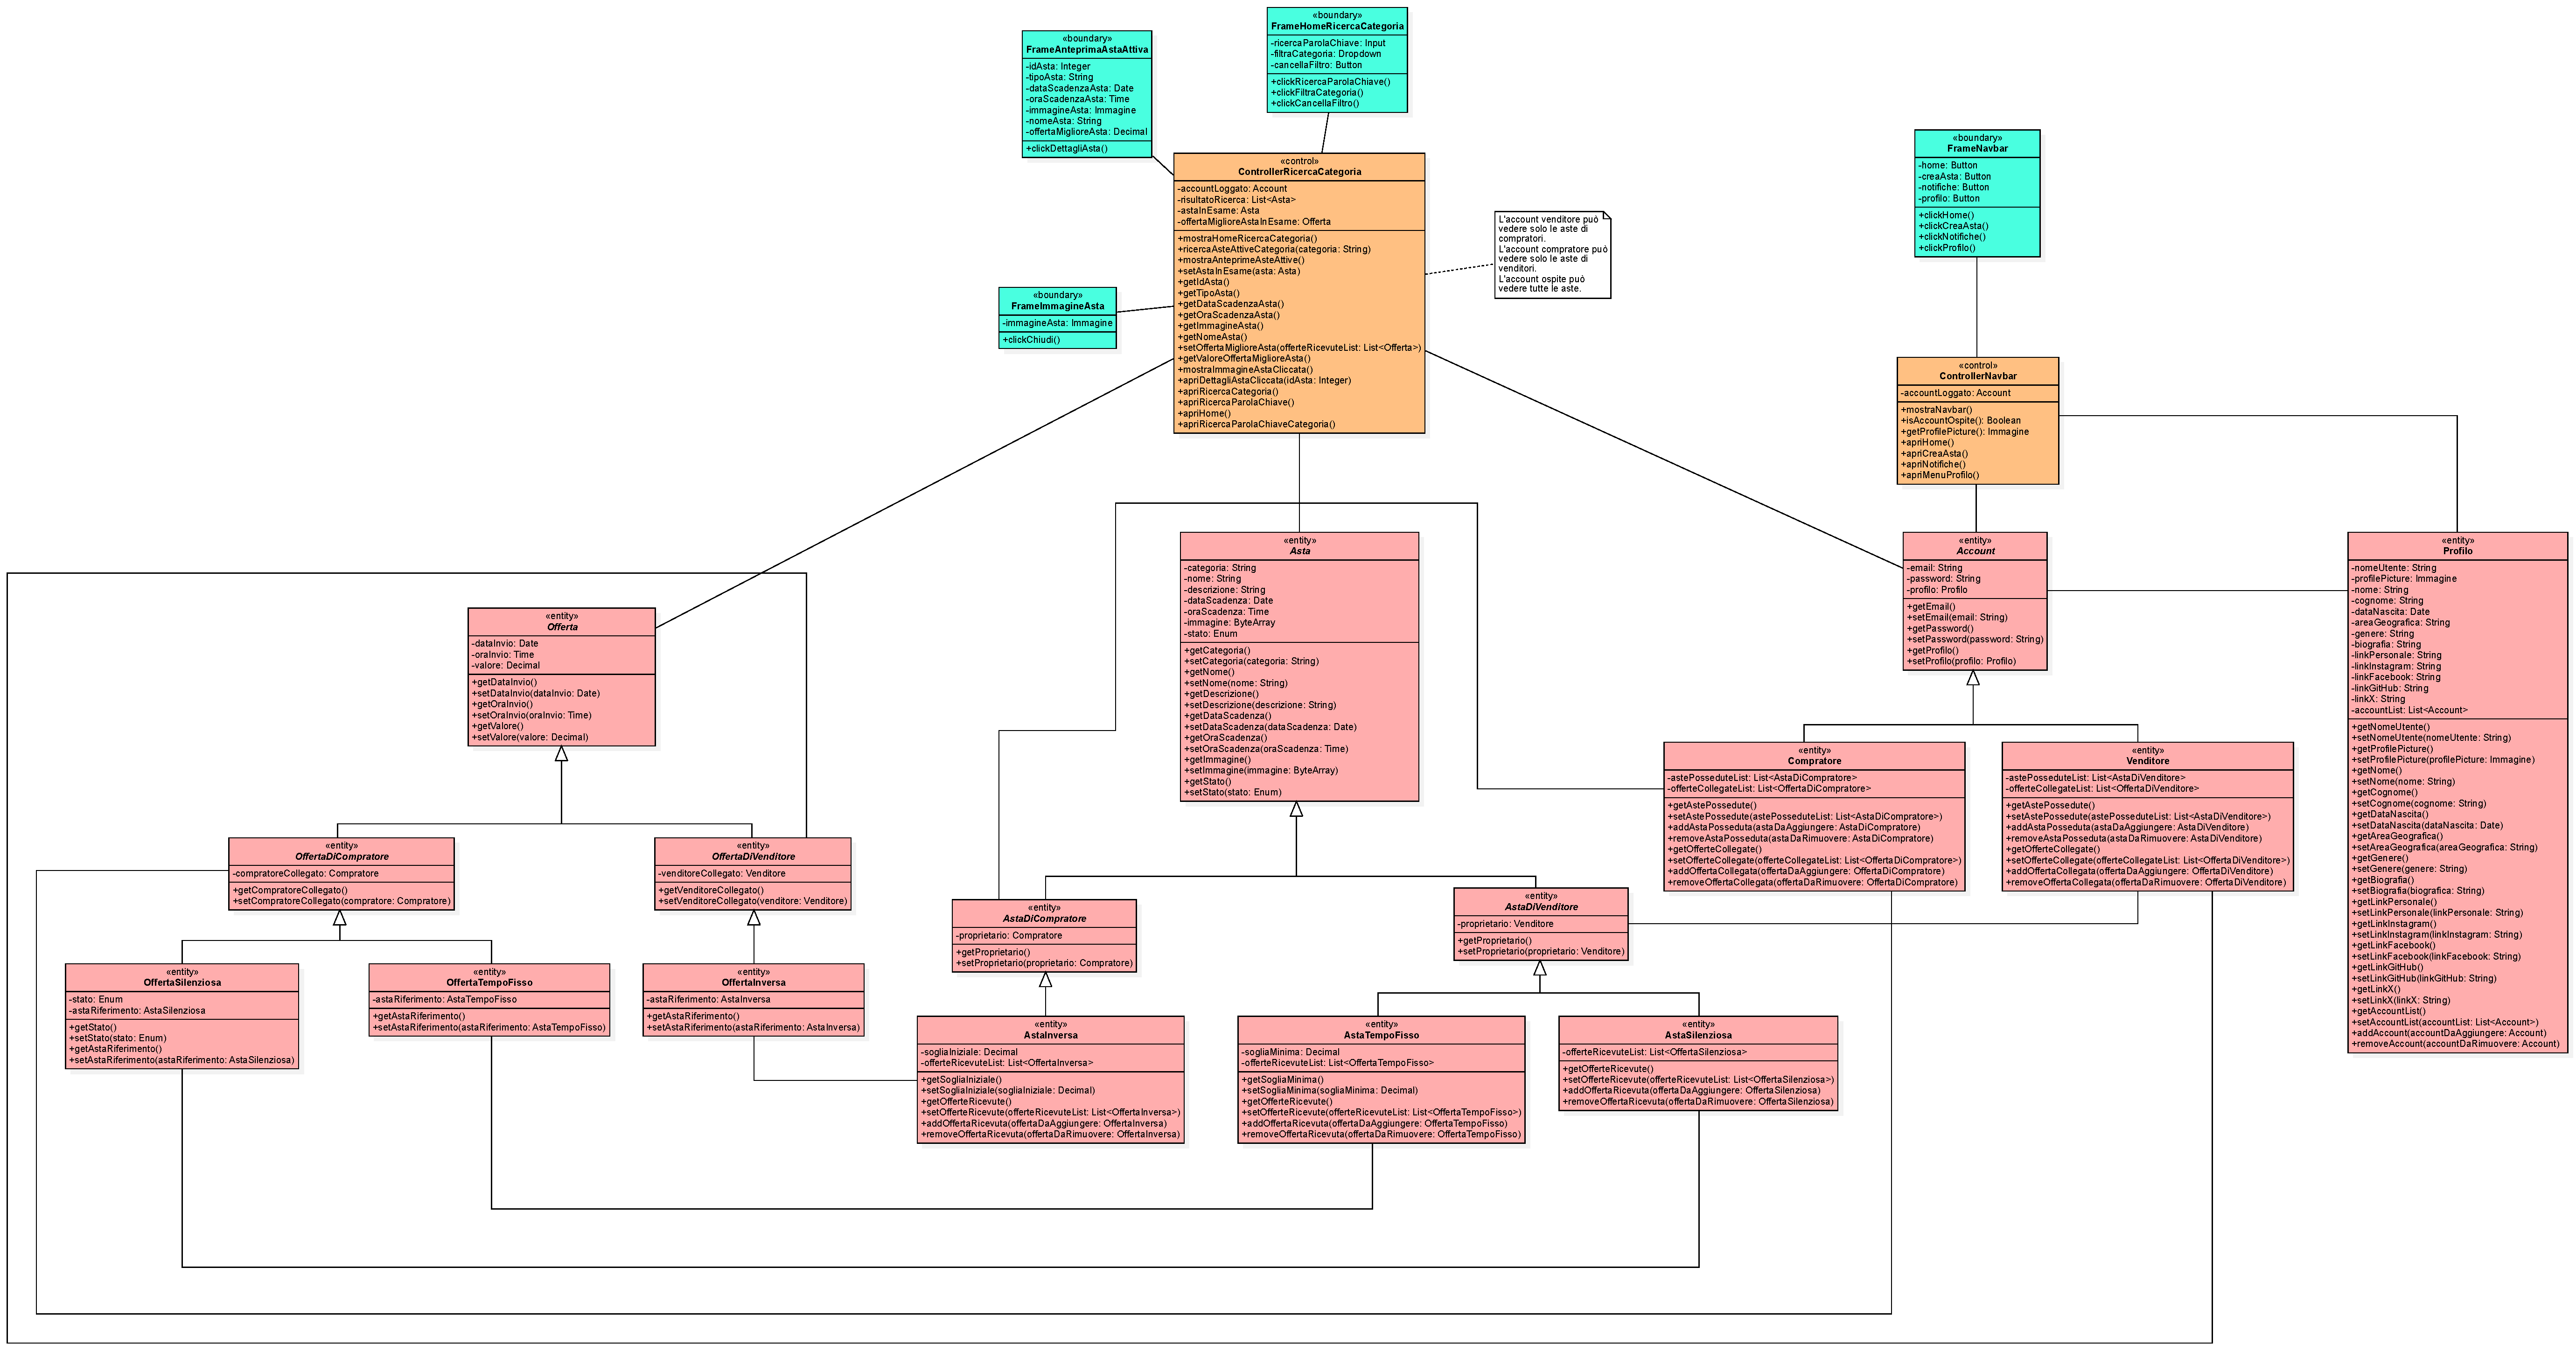
\includegraphics[width=1\linewidth]{Immagini/Diagrammi/Class Diagram/Analisi/Utente generico/RicercaCategoria.pdf}
                \caption{Ricerca per categoria}
            \end{figure}
            
            \begin{figure}[htbp!]
                \centering
                    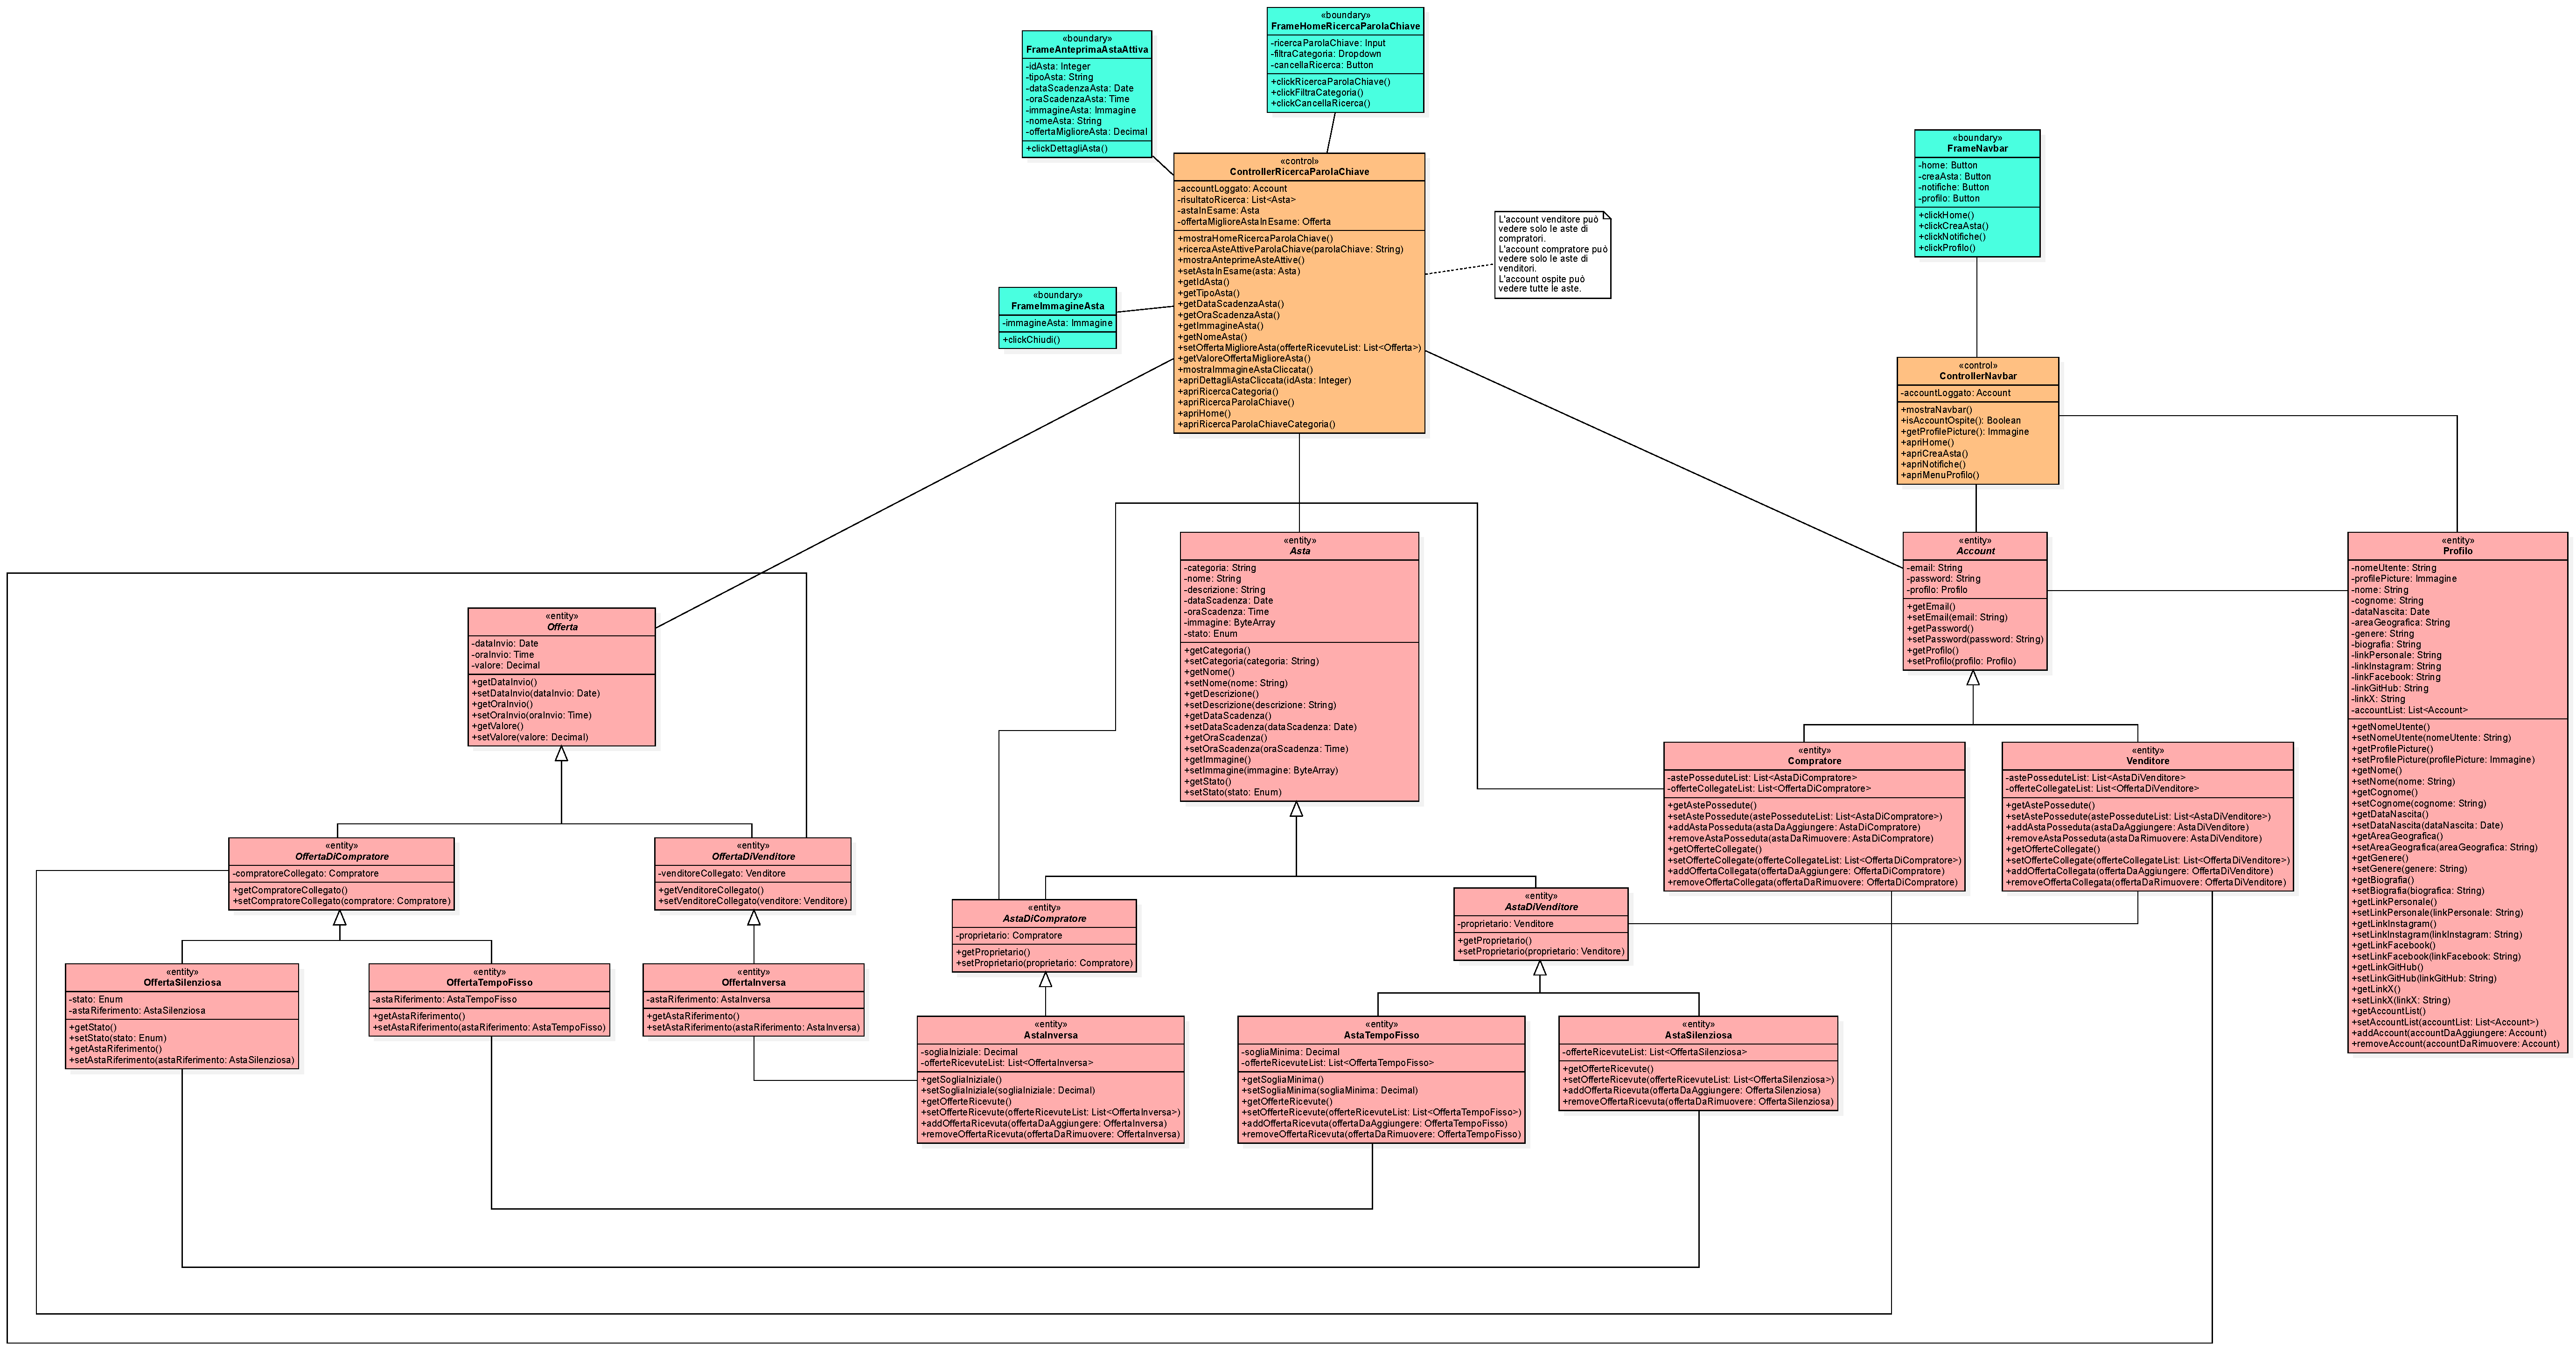
\includegraphics[width=1\linewidth]{Immagini/Diagrammi/Class Diagram/Analisi/Utente generico/RicercaParolaChiave.pdf}
                \caption{Ricerca per parola chiave}
            \end{figure}
            
            \begin{figure}[htbp!]
                \centering
                    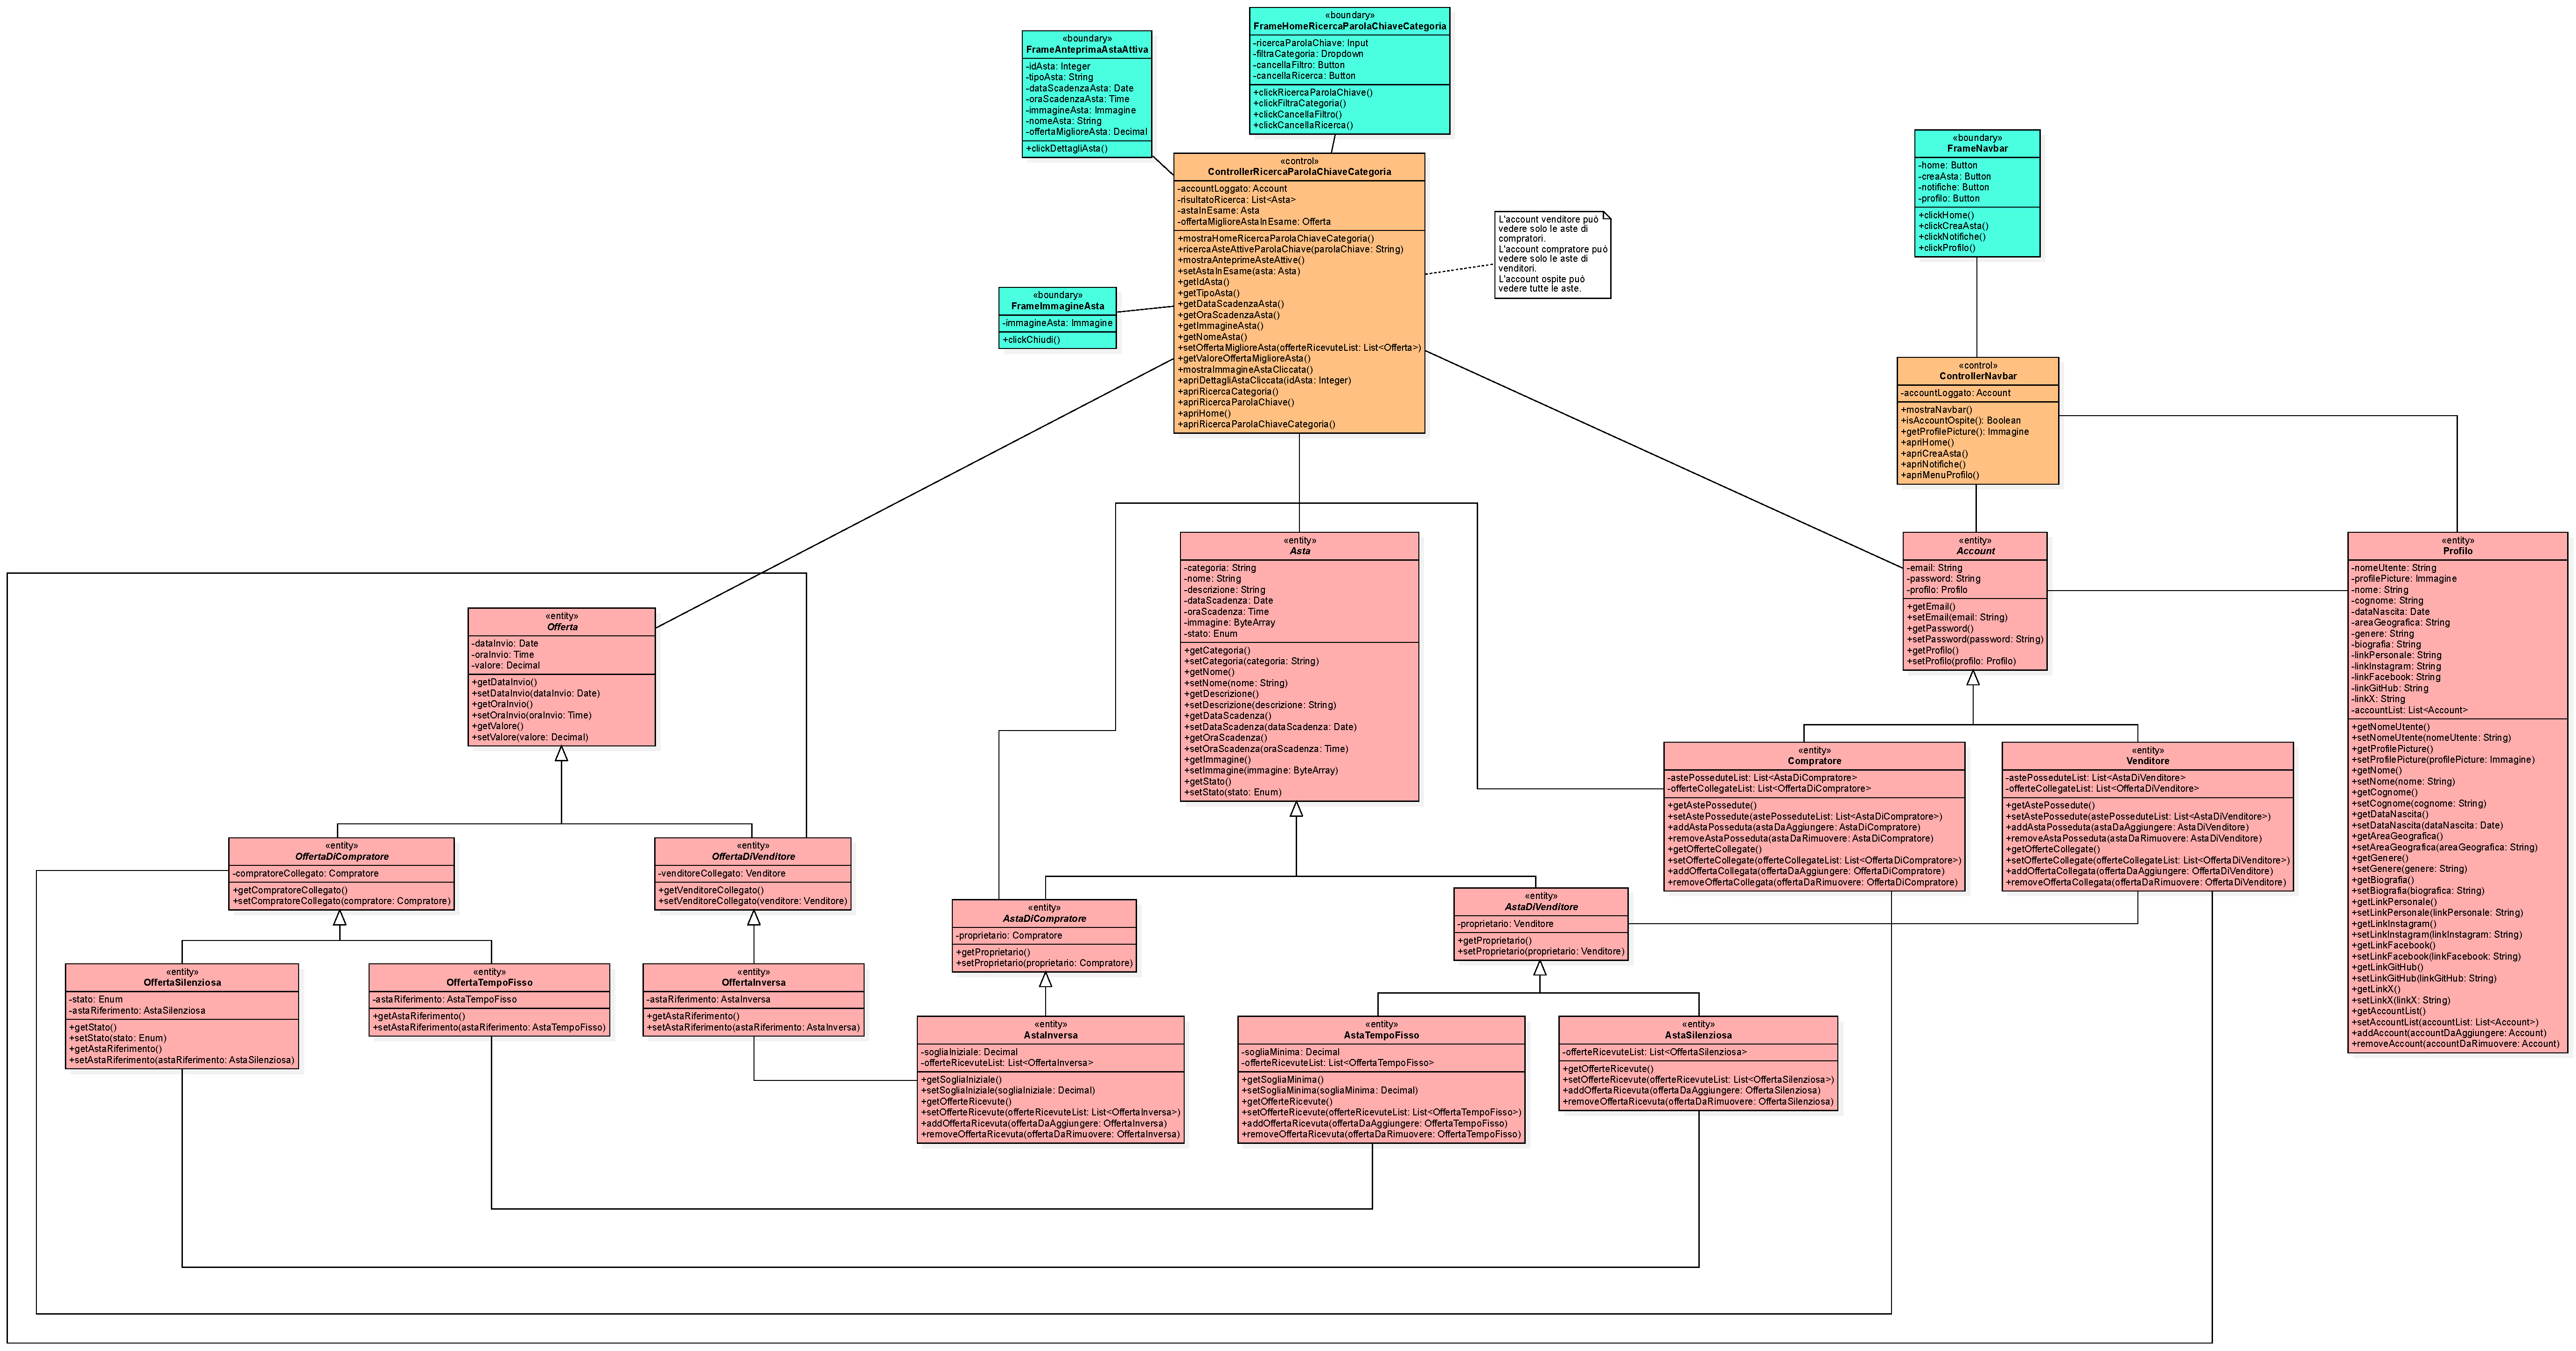
\includegraphics[width=1\linewidth]{Immagini/Diagrammi/Class Diagram/Analisi/Utente generico/RicercaParolaChiaveCategoria.pdf}
                \caption{Ricerca per parola chiave e categoria}
            \end{figure}
            
            \begin{figure}[htbp!]
                \centering
                    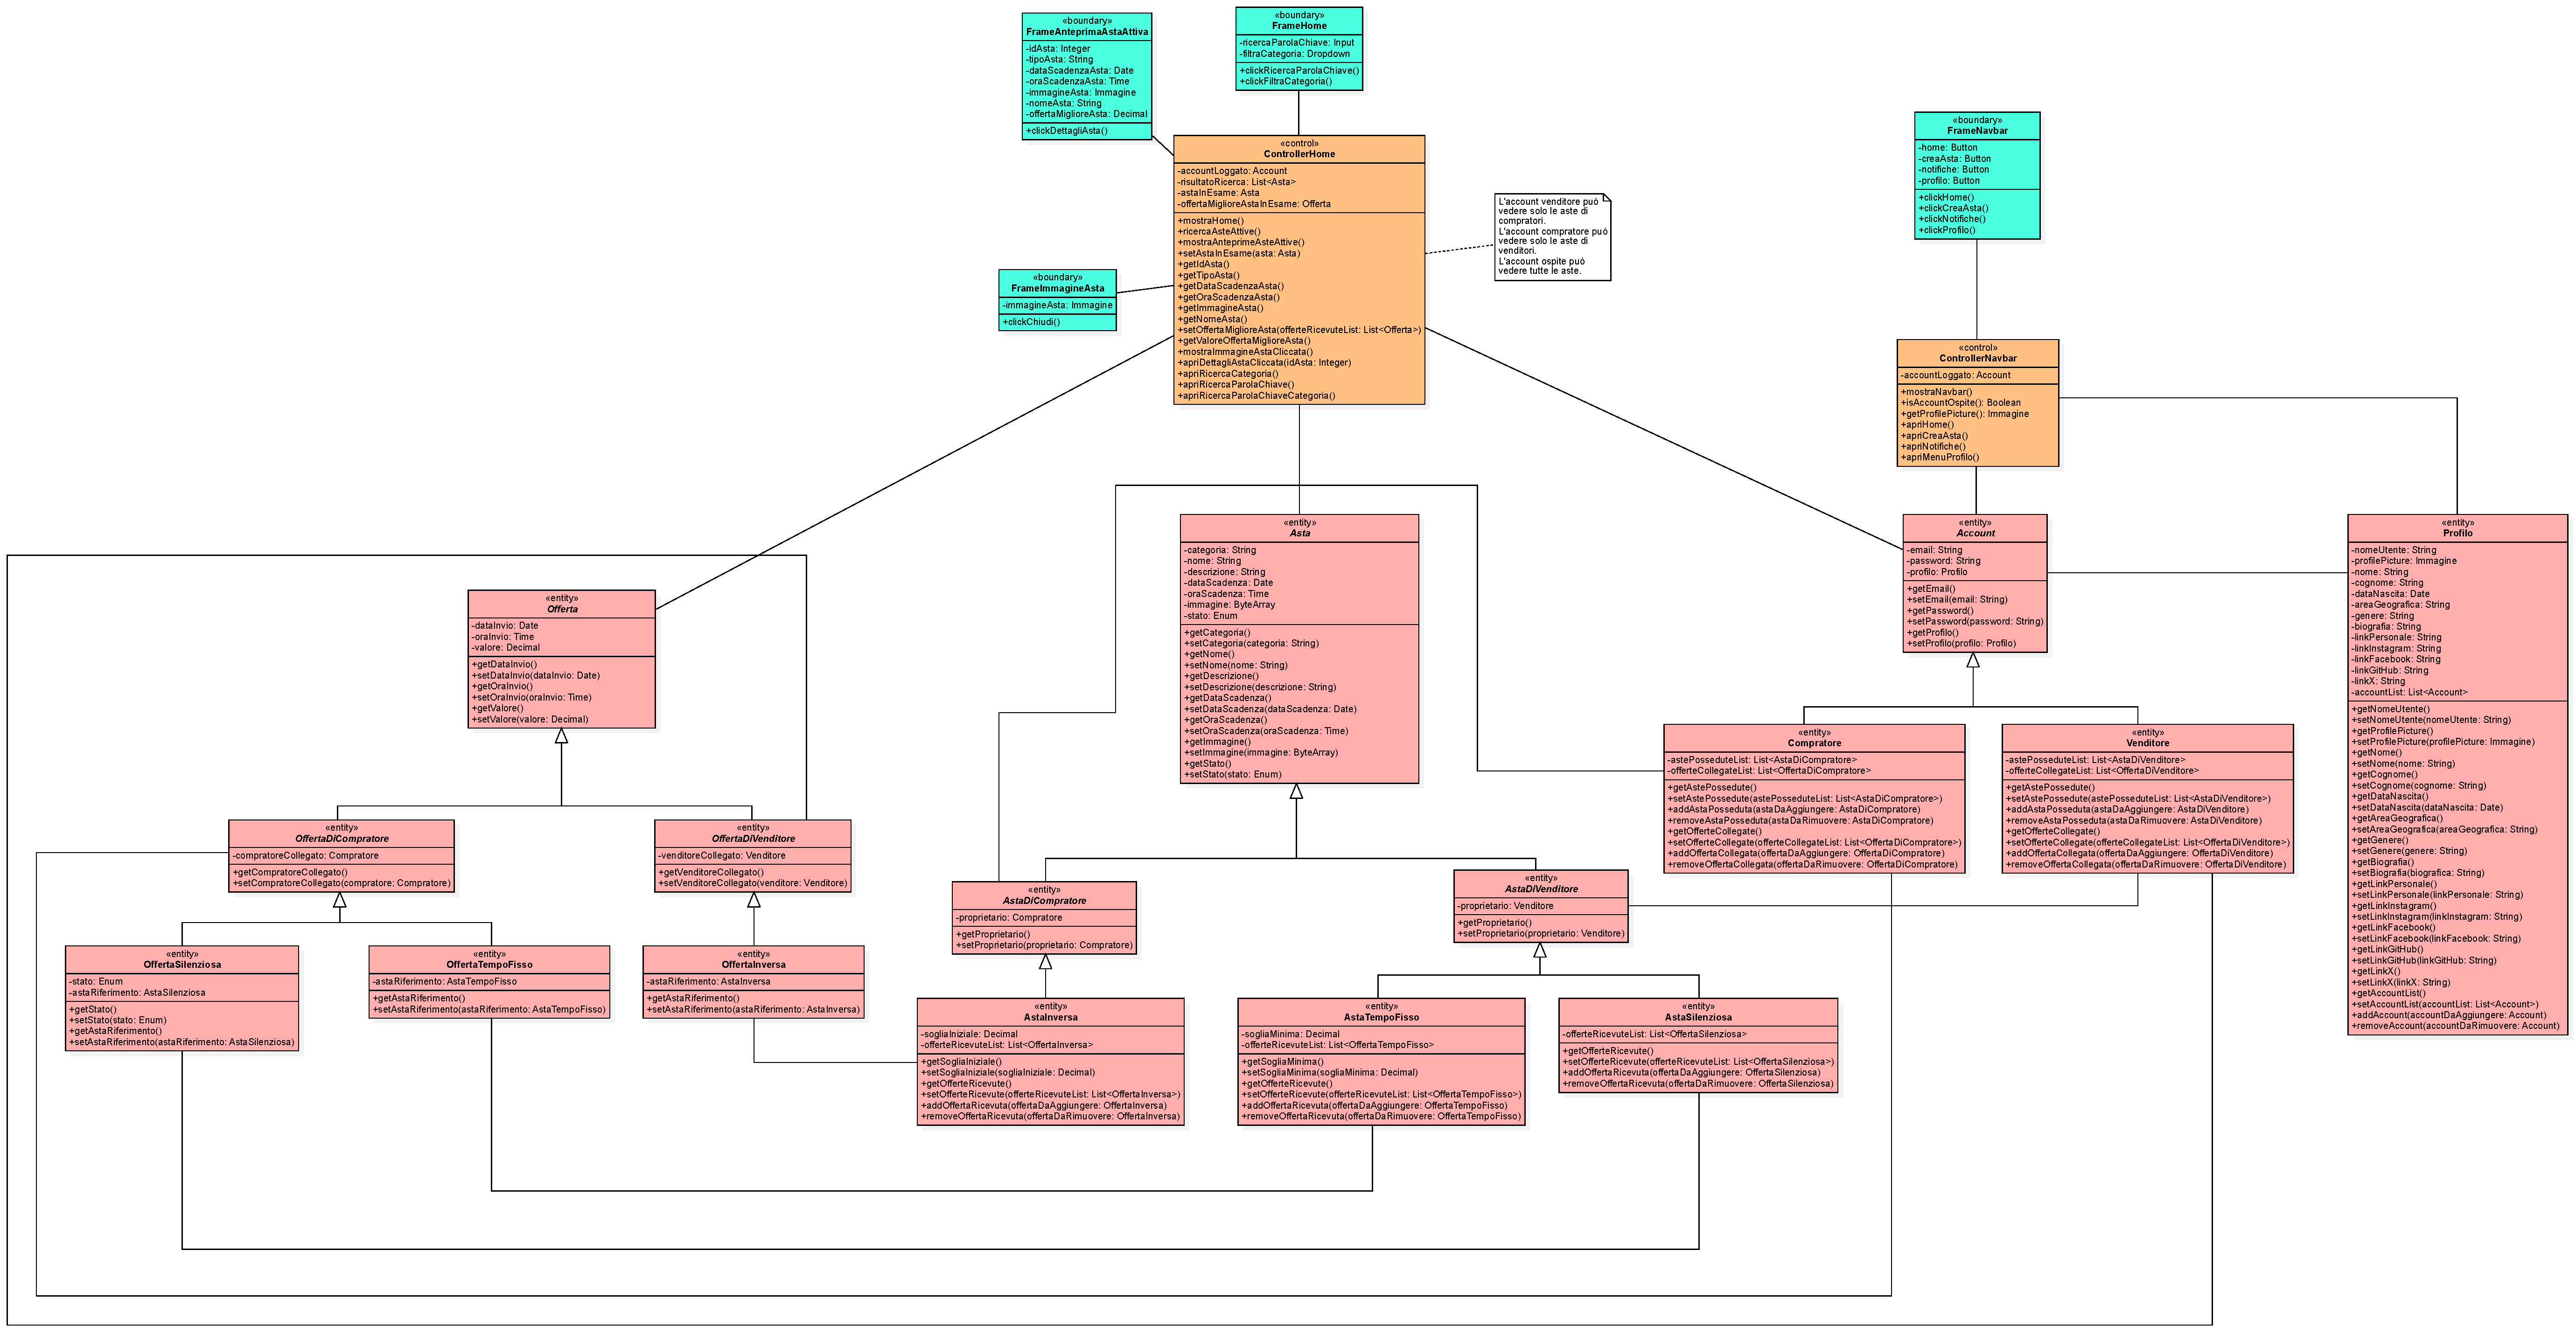
\includegraphics[width=1\linewidth]{Immagini/Diagrammi/Class Diagram/Analisi/Utente generico/VisualizzaAsteAttive.pdf}
                \caption{Visualizza aste attive}
            \end{figure}
            
            \begin{figure}[htbp!]
                \centering
                    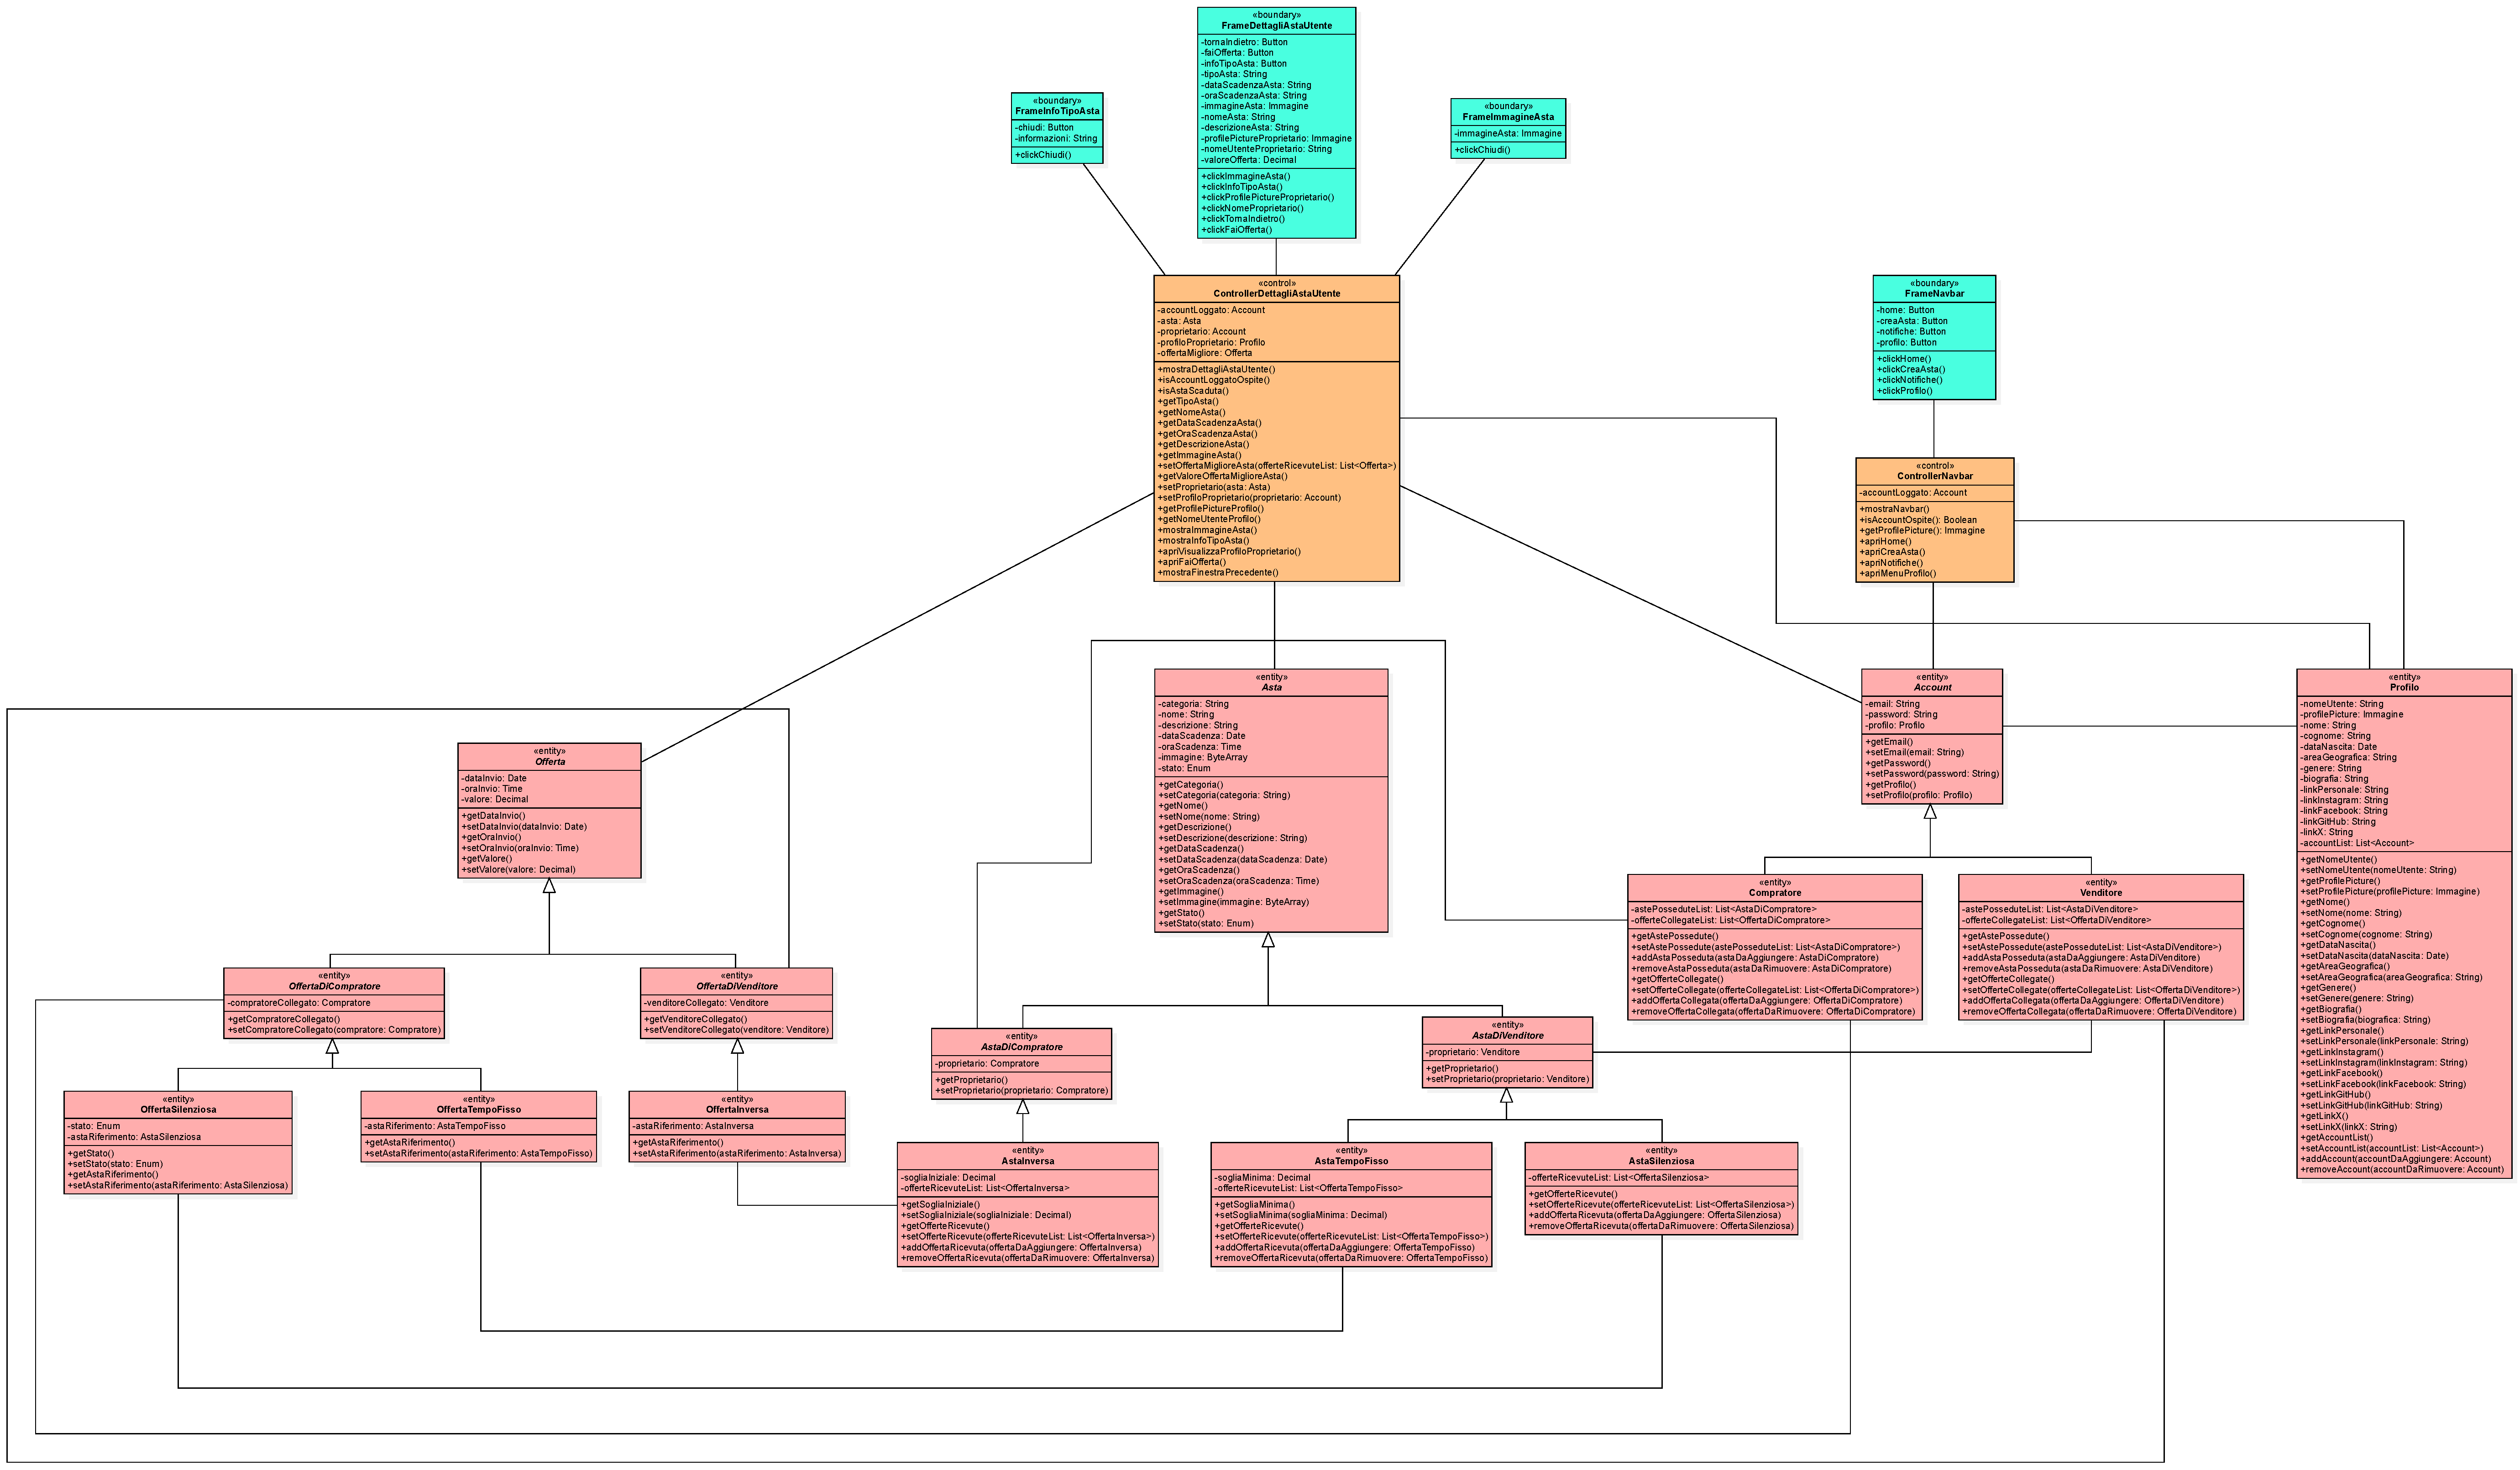
\includegraphics[width=1\linewidth]{Immagini/Diagrammi/Class Diagram/Analisi/Utente generico/VisualizzaDettagliAstaUtente.pdf}
                \caption{Visualizza dettagli asta di un altro utente}
            \end{figure}
            
            \begin{figure}[htbp!]
                \centering
                    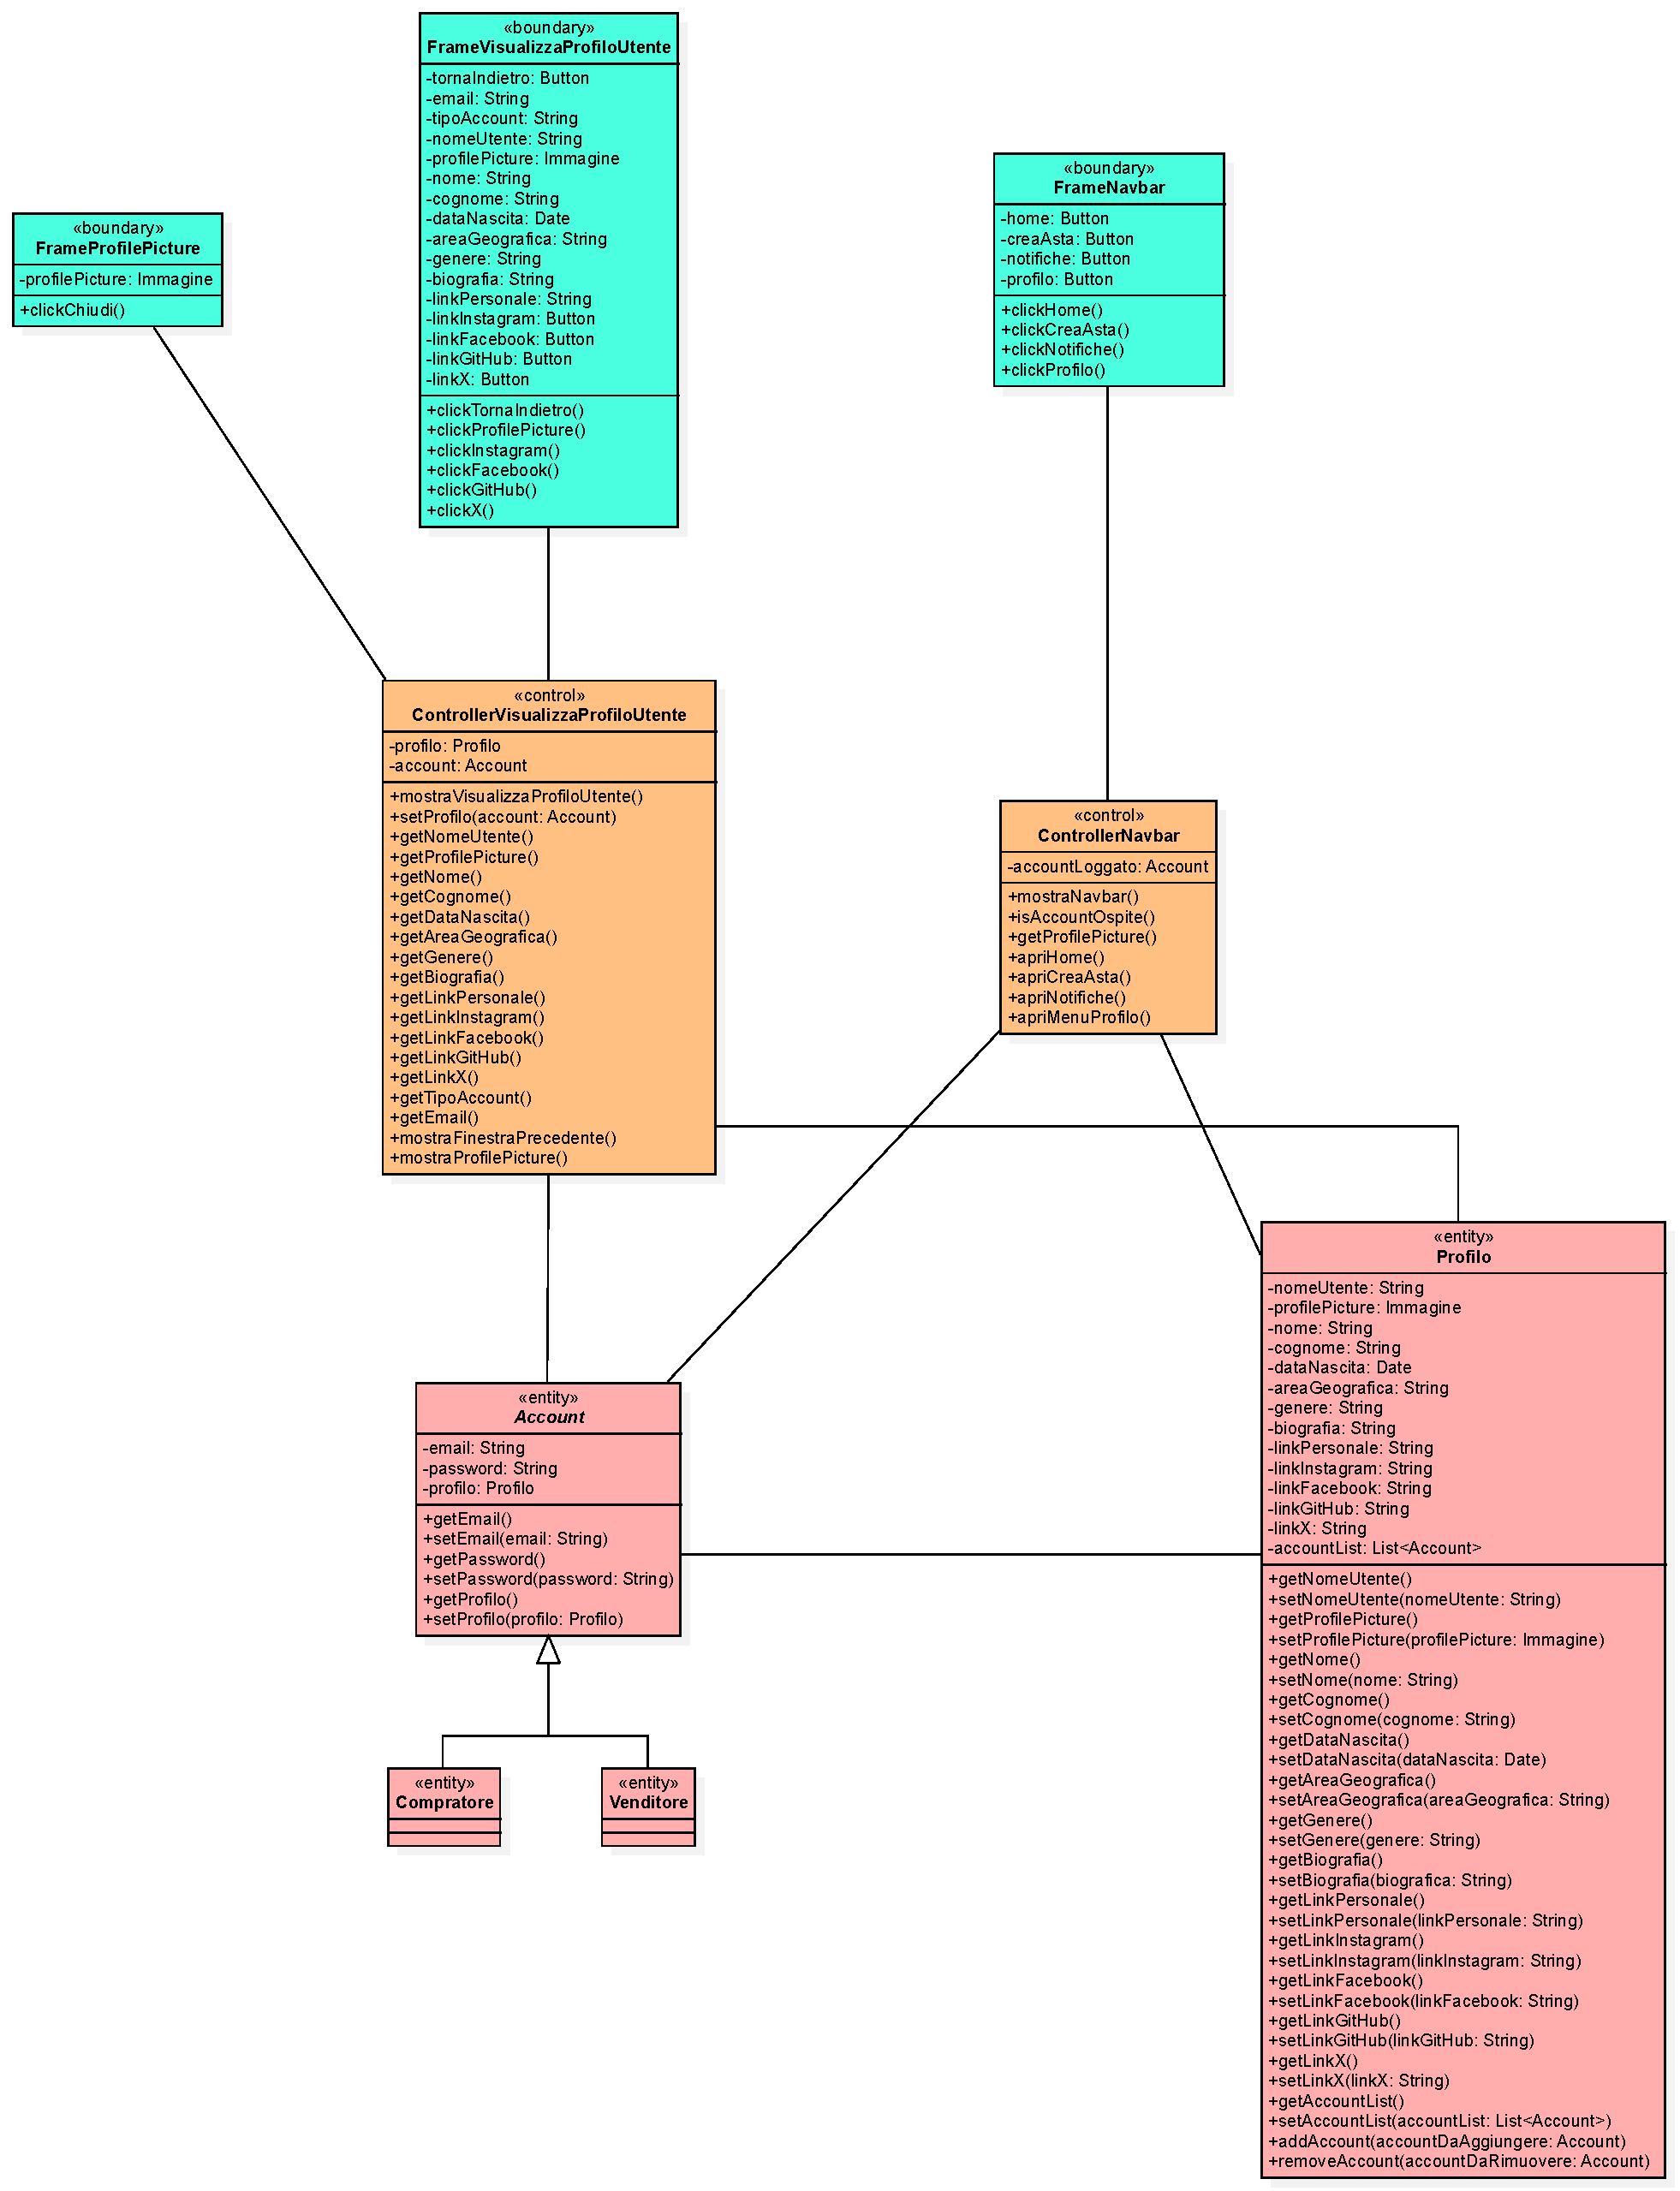
\includegraphics[width=1\linewidth]{Immagini/Diagrammi/Class Diagram/Analisi/Utente generico/VisualizzaProfiloUtente.pdf}
                \caption{Visualizza profilo utente}
            \end{figure}
            
            \begin{figure}[htbp!]
                \centering
                    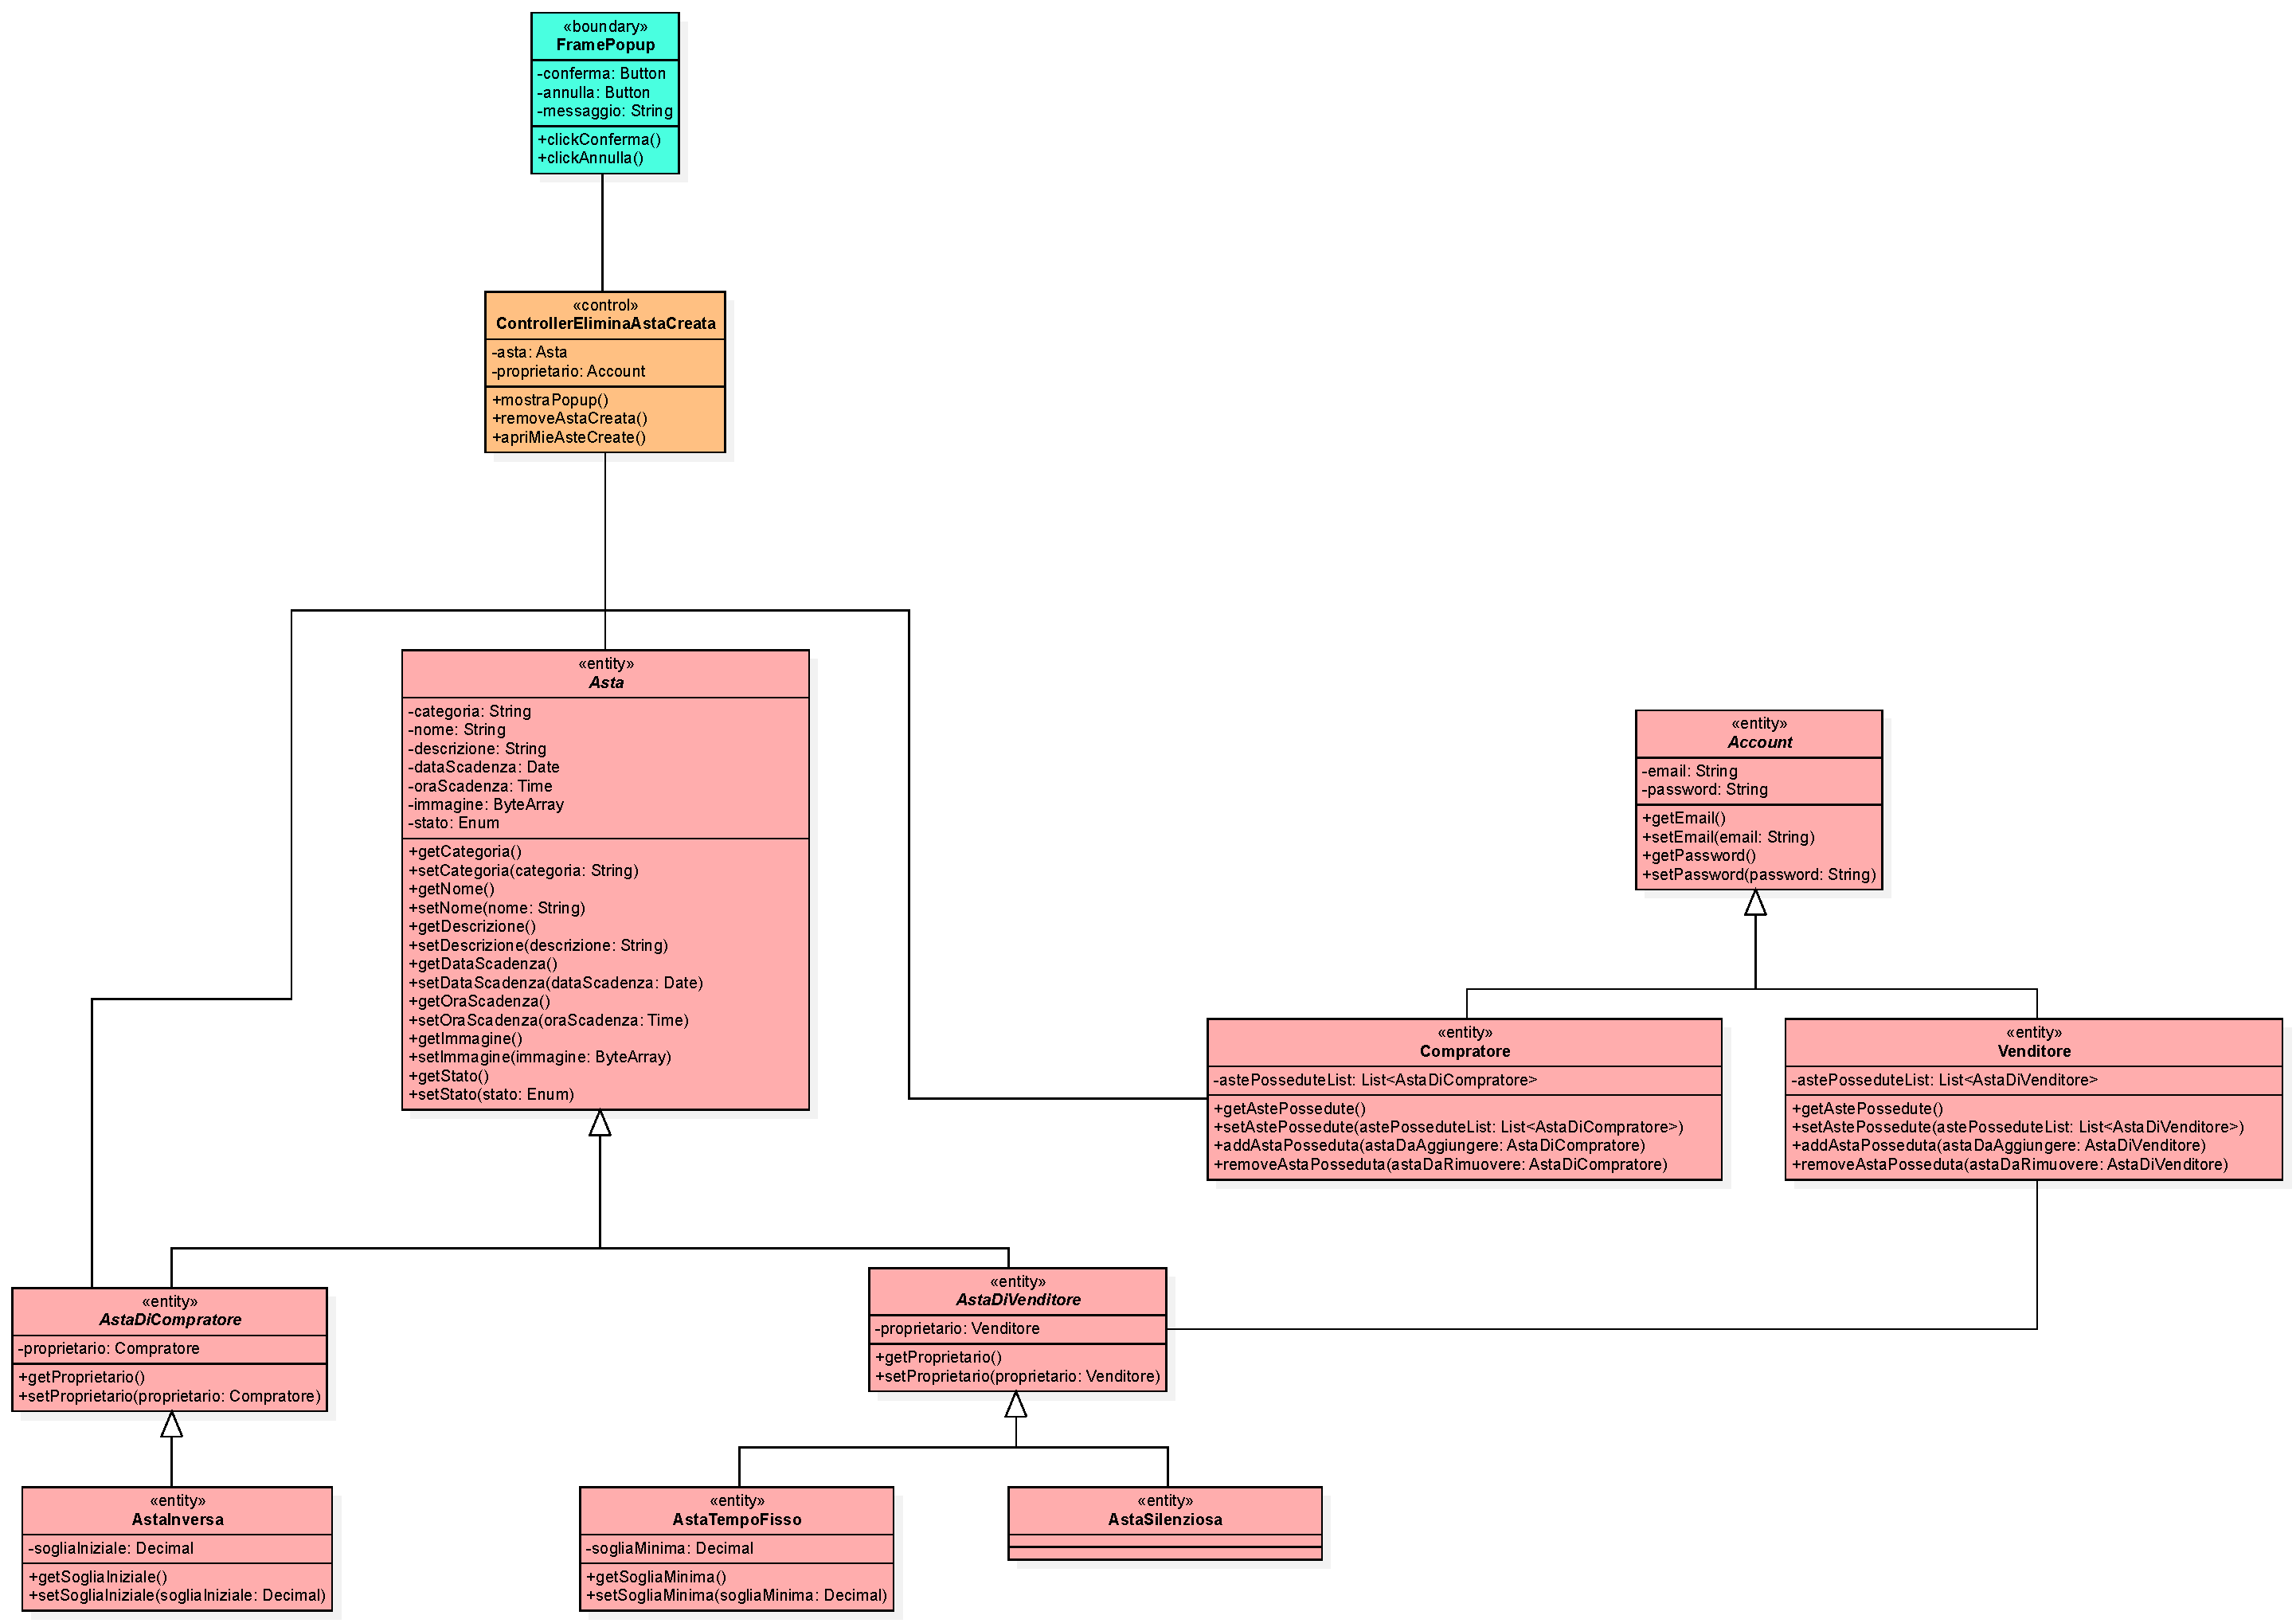
\includegraphics[width=1\linewidth]{Immagini/Diagrammi/Class Diagram/Analisi/Utente che ha effettuato l'accesso/EliminaAsta.pdf}
                \caption{Elimina asta creata}
            \end{figure}
            
            \begin{figure}[htbp!]
                \centering
                    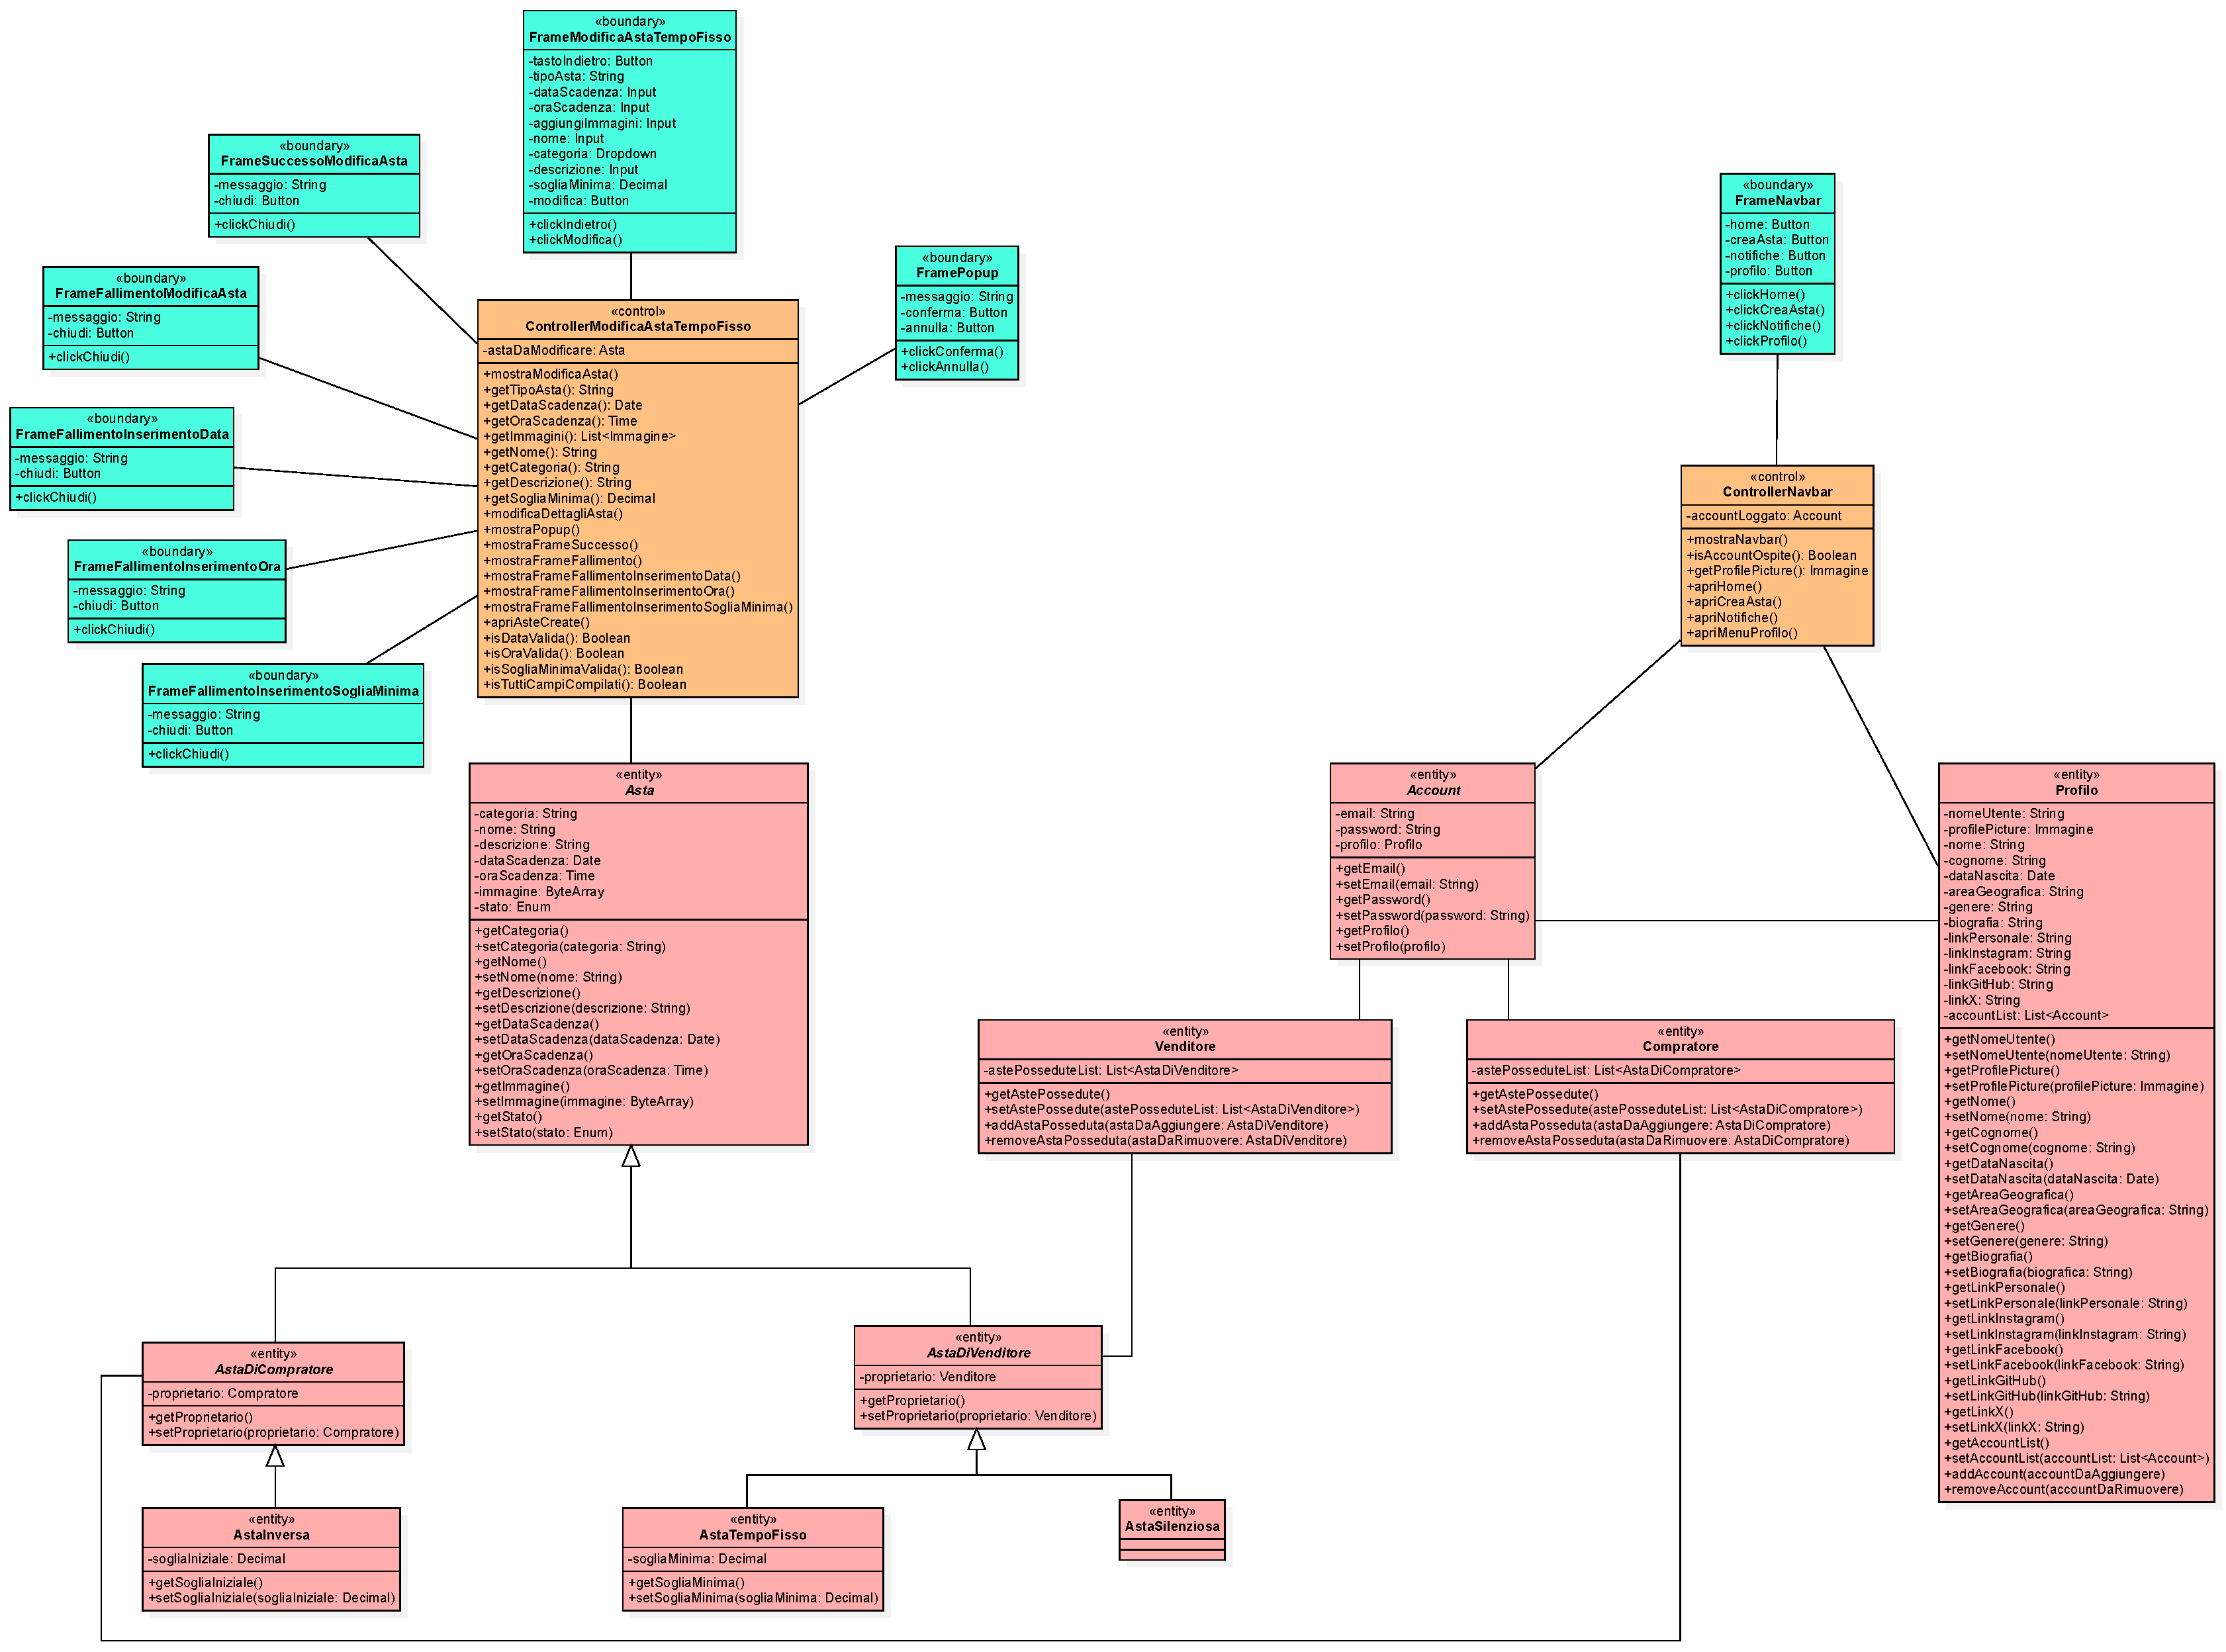
\includegraphics[width=1\linewidth]{Immagini/Diagrammi/Class Diagram/Analisi/Utente che ha effettuato l'accesso/ModificaAstaTempoFisso.pdf}
                \caption{Modifica asta a tempo fisso}
            \end{figure}
            
            \begin{figure}[htbp!]
                \centering
                    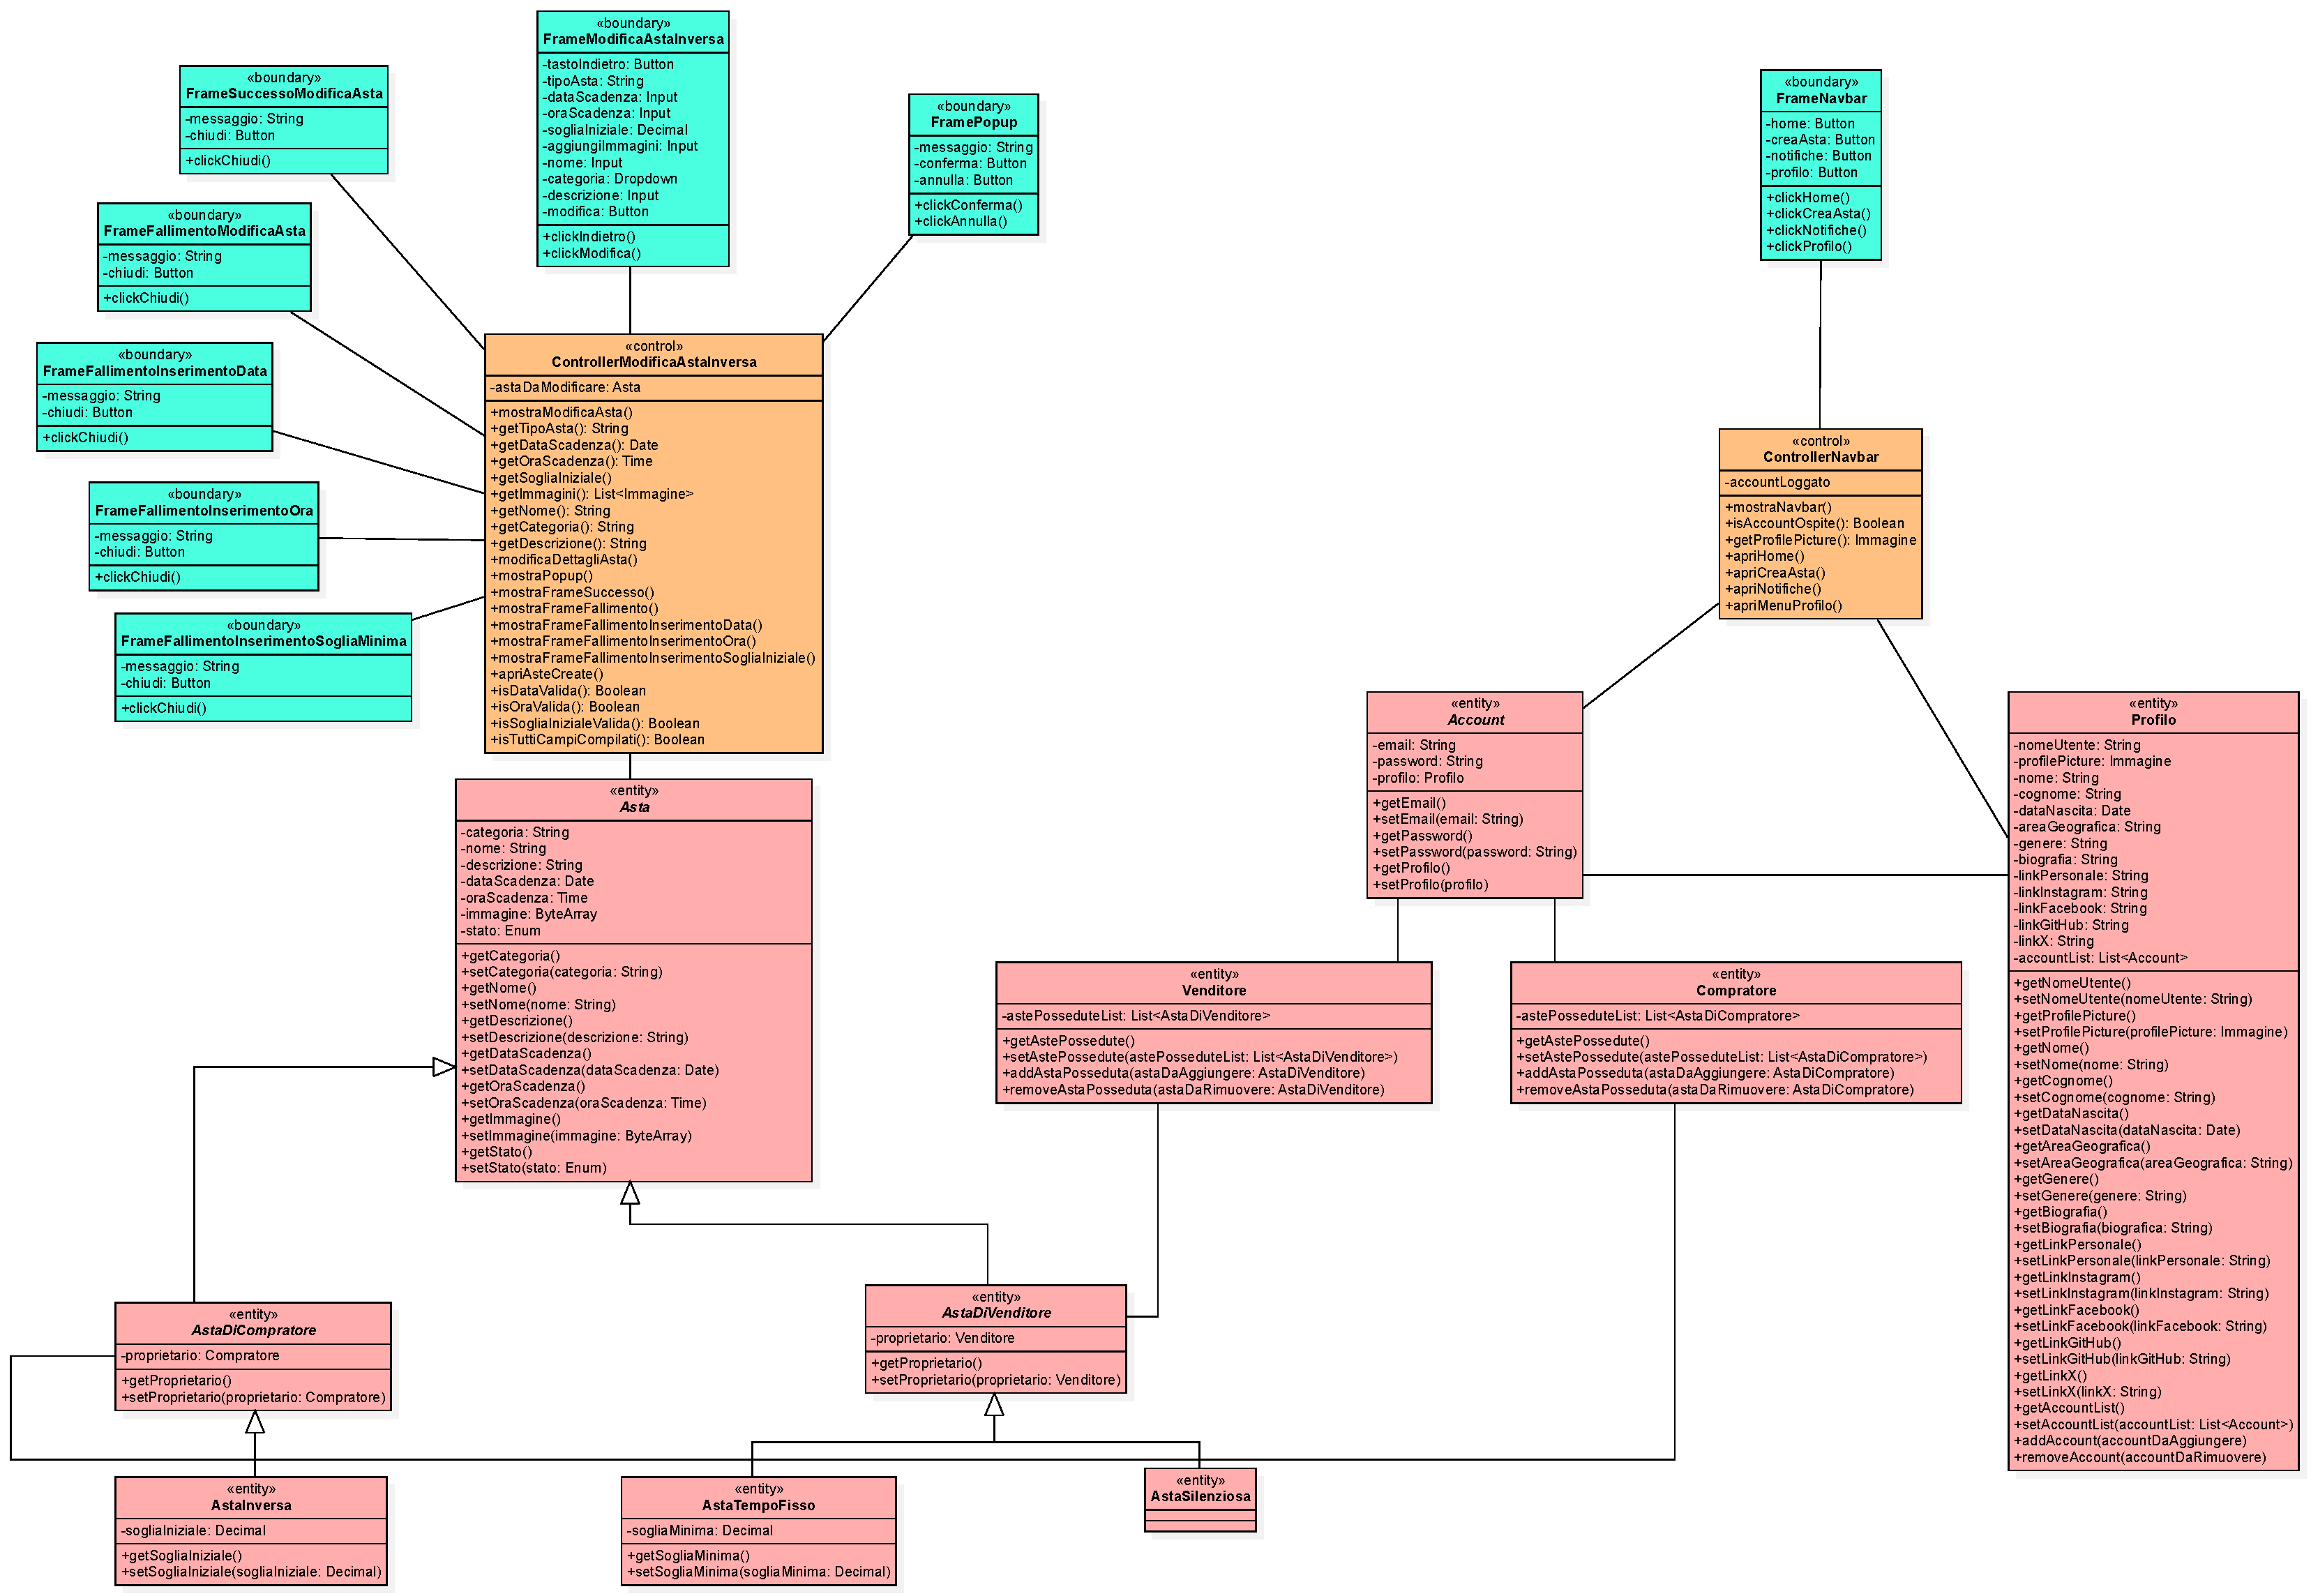
\includegraphics[width=1\linewidth]{Immagini/Diagrammi/Class Diagram/Analisi/Utente che ha effettuato l'accesso/ModificaAstaInversa.pdf}
                \caption{Modifica asta inversa}
            \end{figure}
            
            \begin{figure}[htbp!]
                \centering
                    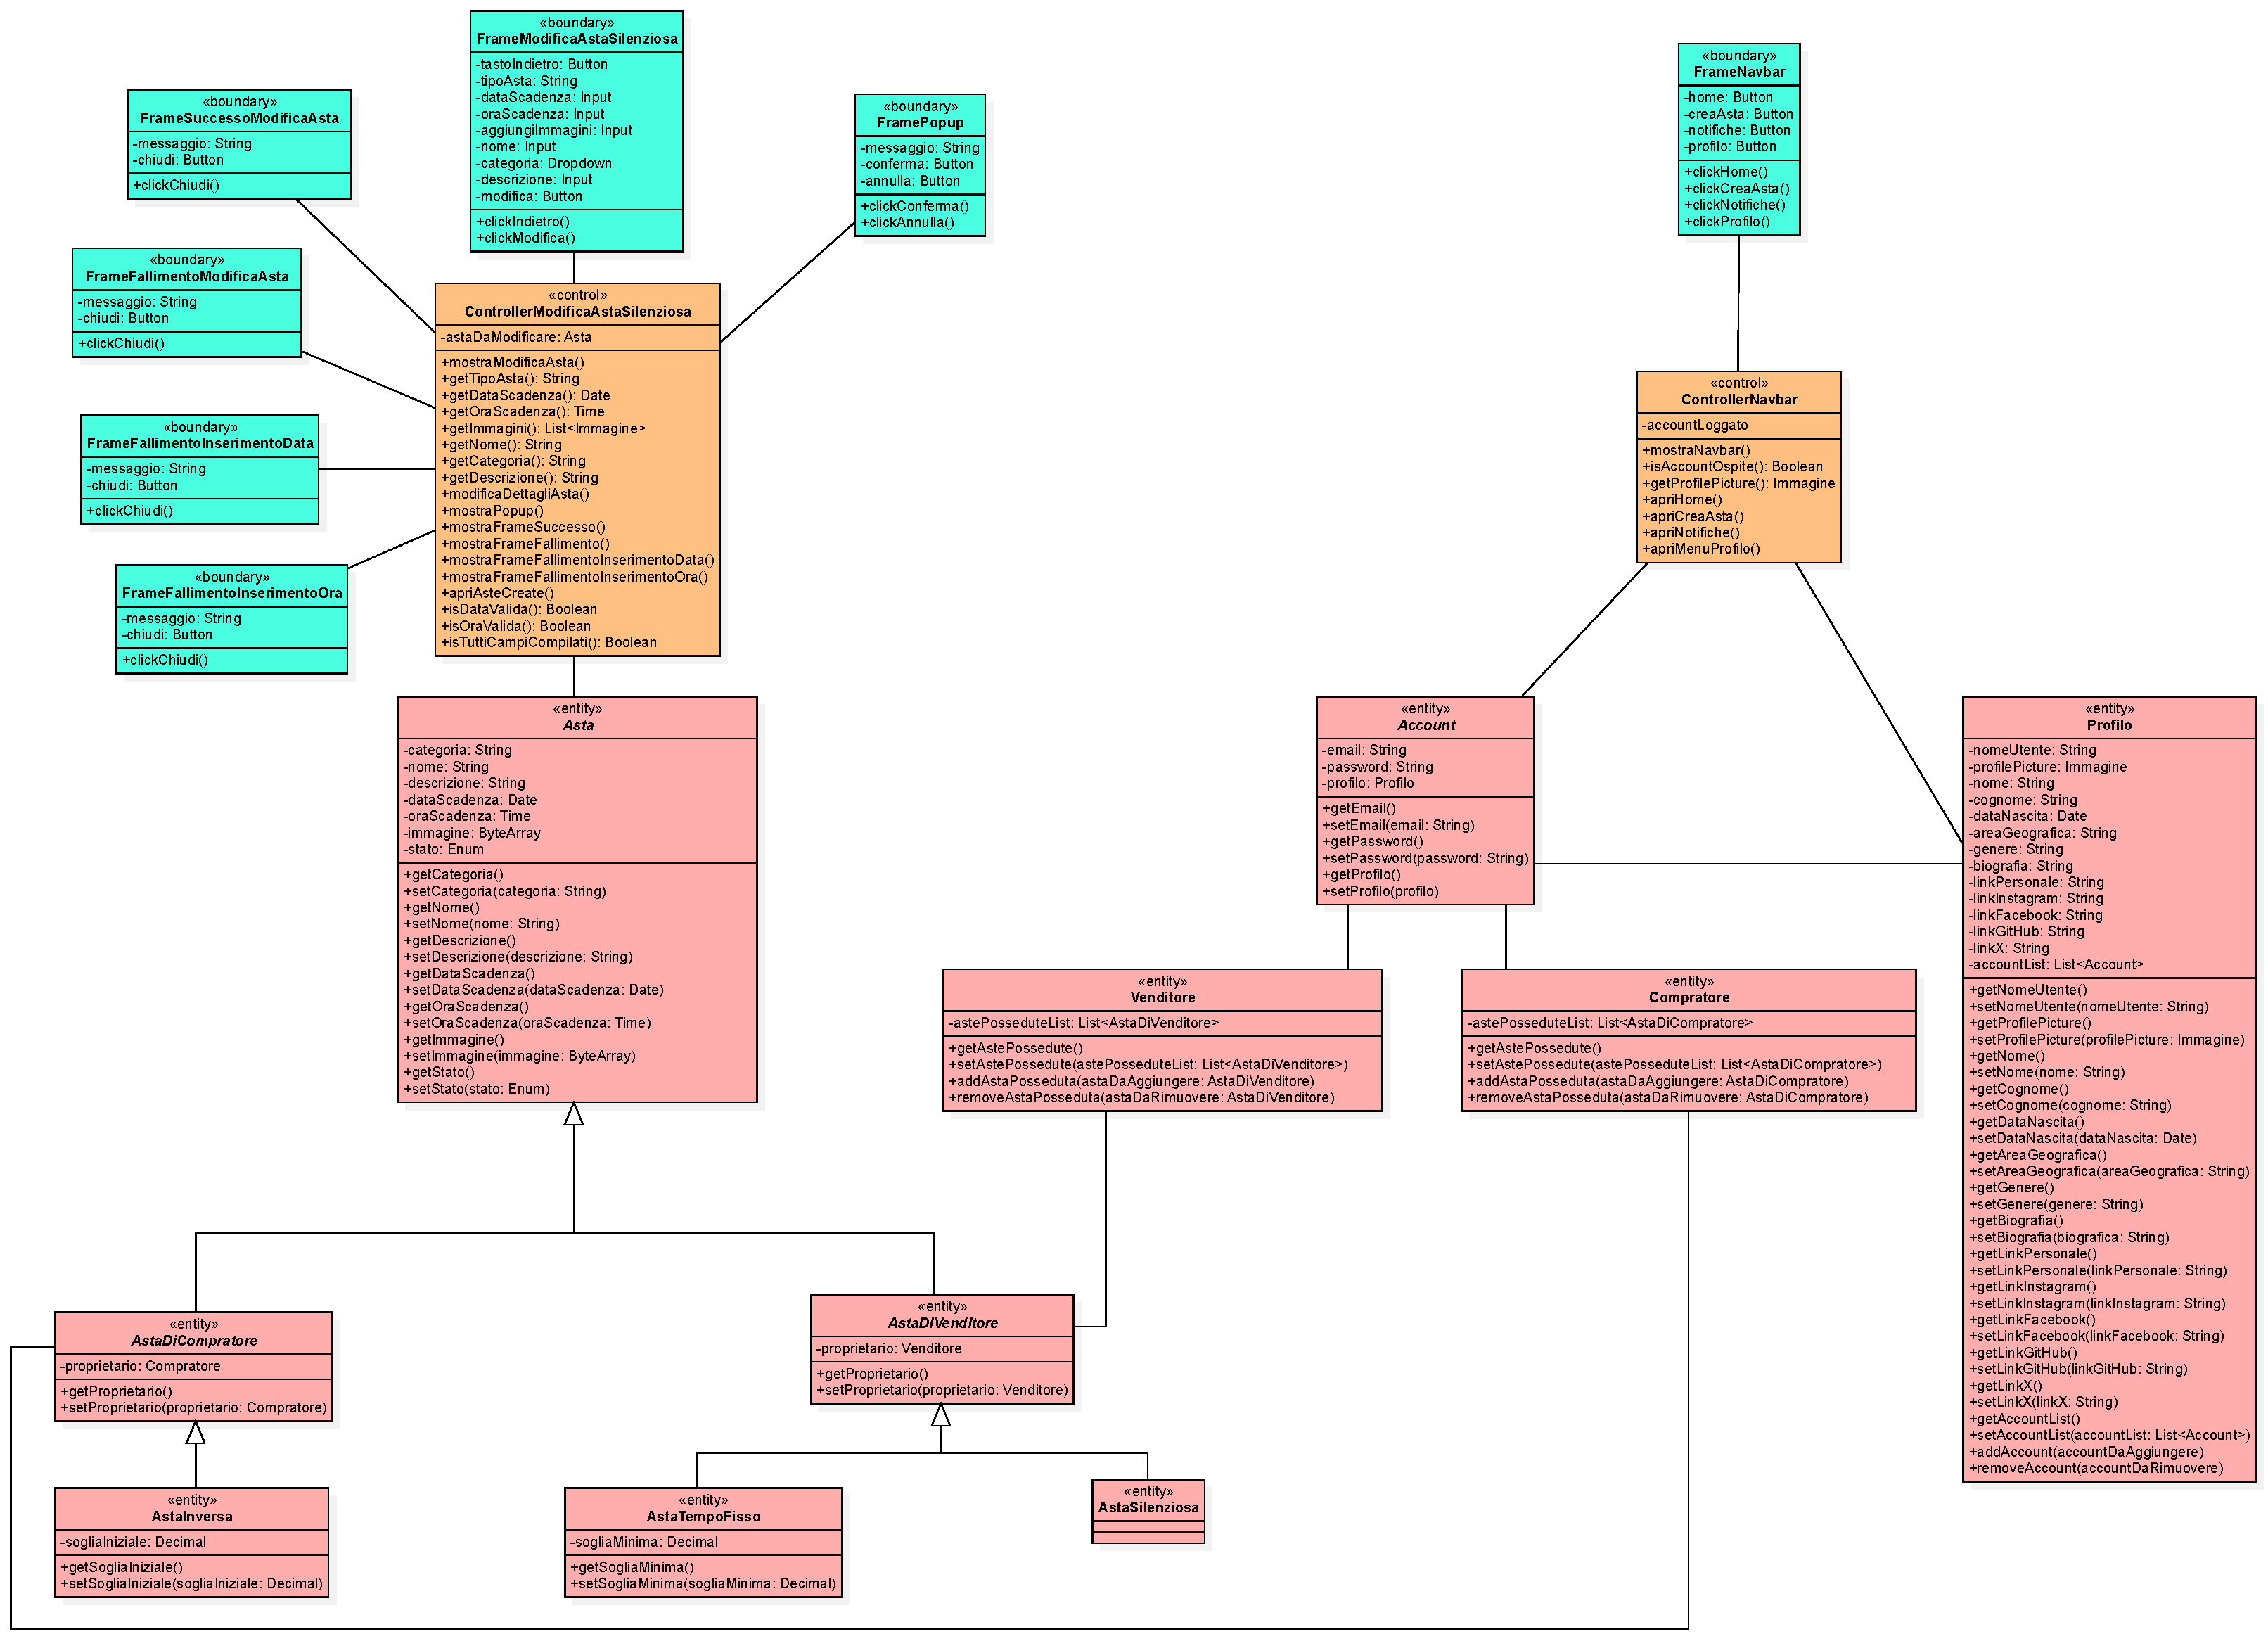
\includegraphics[width=1\linewidth]{Immagini/Diagrammi/Class Diagram/Analisi/Utente che ha effettuato l'accesso/ModificaAstaSilenziosa.pdf}
                \caption{Modifica asta silenziosa}
            \end{figure}
            
            \begin{figure}[htbp!]
                \centering
                    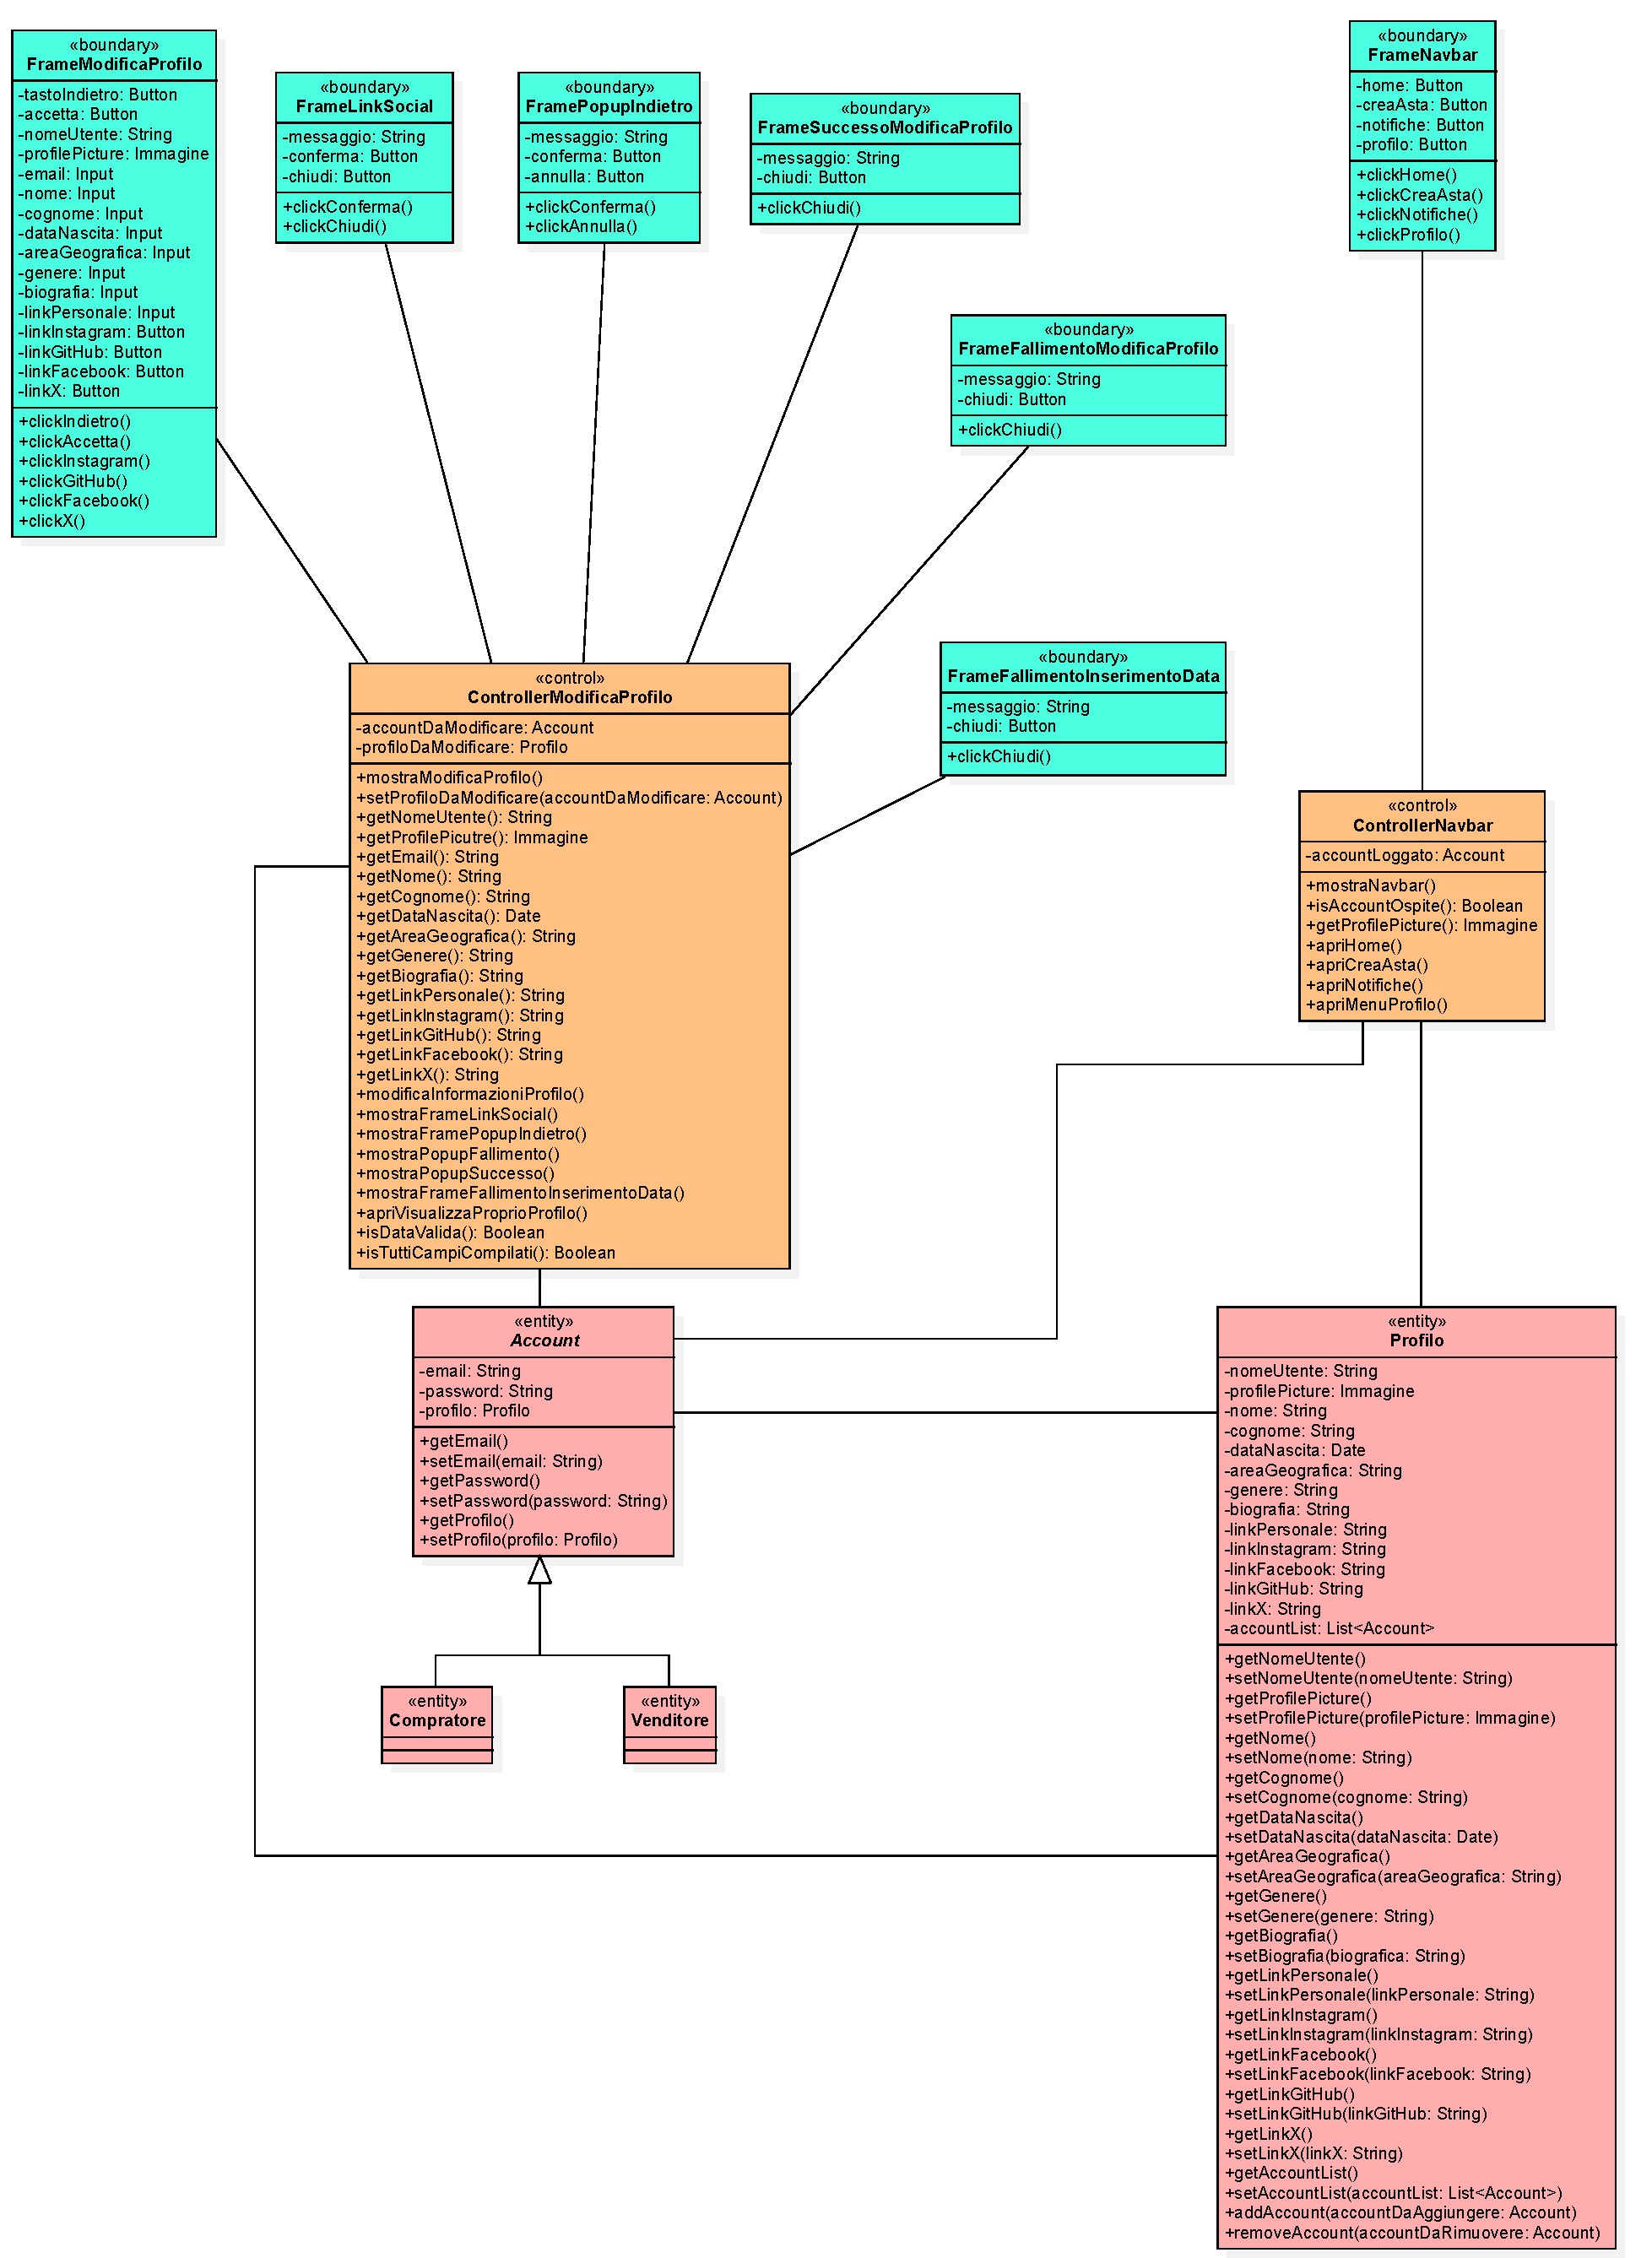
\includegraphics[width=0.8\linewidth]{Immagini/Diagrammi/Class Diagram/Analisi/Utente che ha effettuato l'accesso/ModificaProfilo.pdf}
                \caption{Modifica profilo}
            \end{figure}

            \begin{figure}[htbp!]
                \centering
                    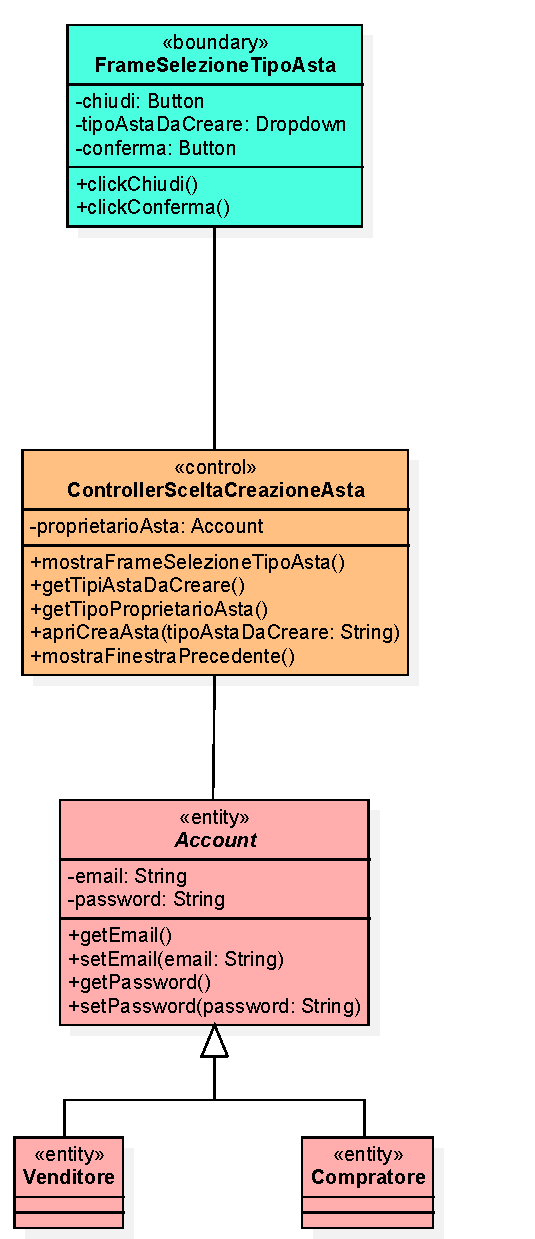
\includegraphics[width=0.5\linewidth]{Immagini/Diagrammi/Class Diagram/Analisi/Utente che ha effettuato l'accesso/SceltaCreazioneAsta.pdf}
                \caption{Scelta tipo di asta da creare}
            \end{figure}
            
            \begin{figure}[htbp!]
                \centering
                    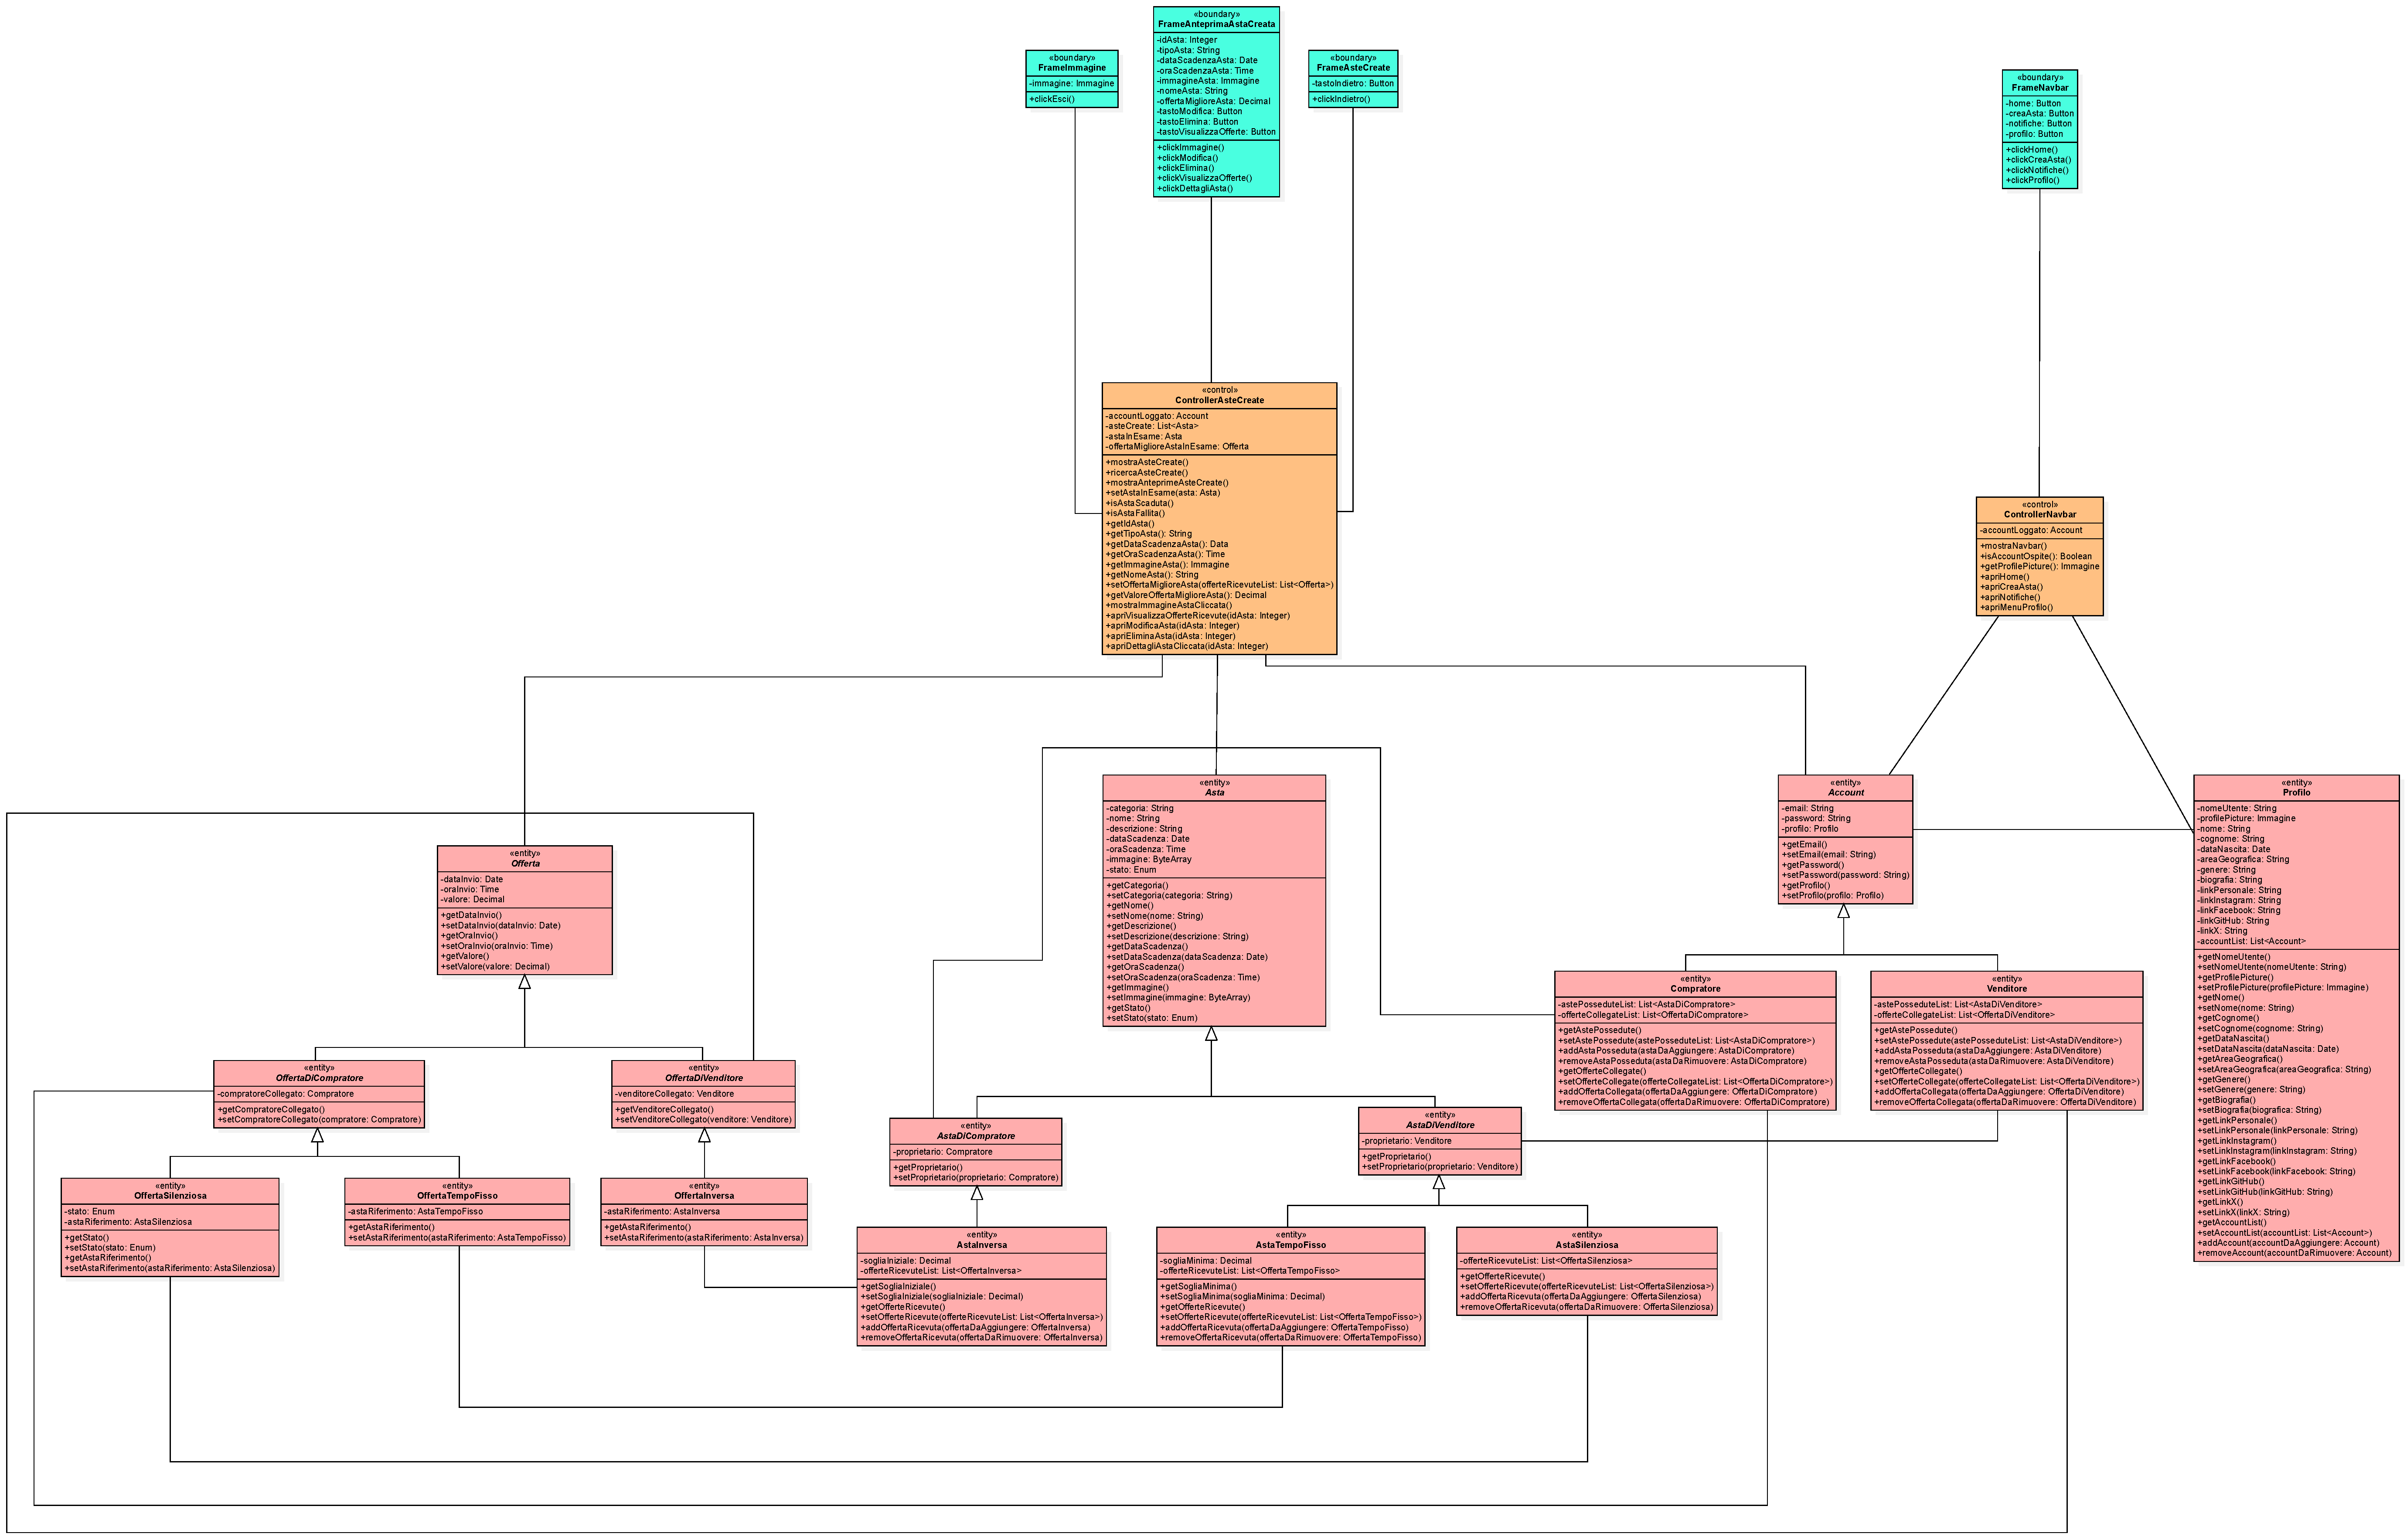
\includegraphics[width=1\linewidth]{Immagini/Diagrammi/Class Diagram/Analisi/Utente che ha effettuato l'accesso/VisualizzaAsteCreate.pdf}
                \caption{Visualizza aste create}
            \end{figure}

            \begin{figure}[htbp!]
                \centering
                    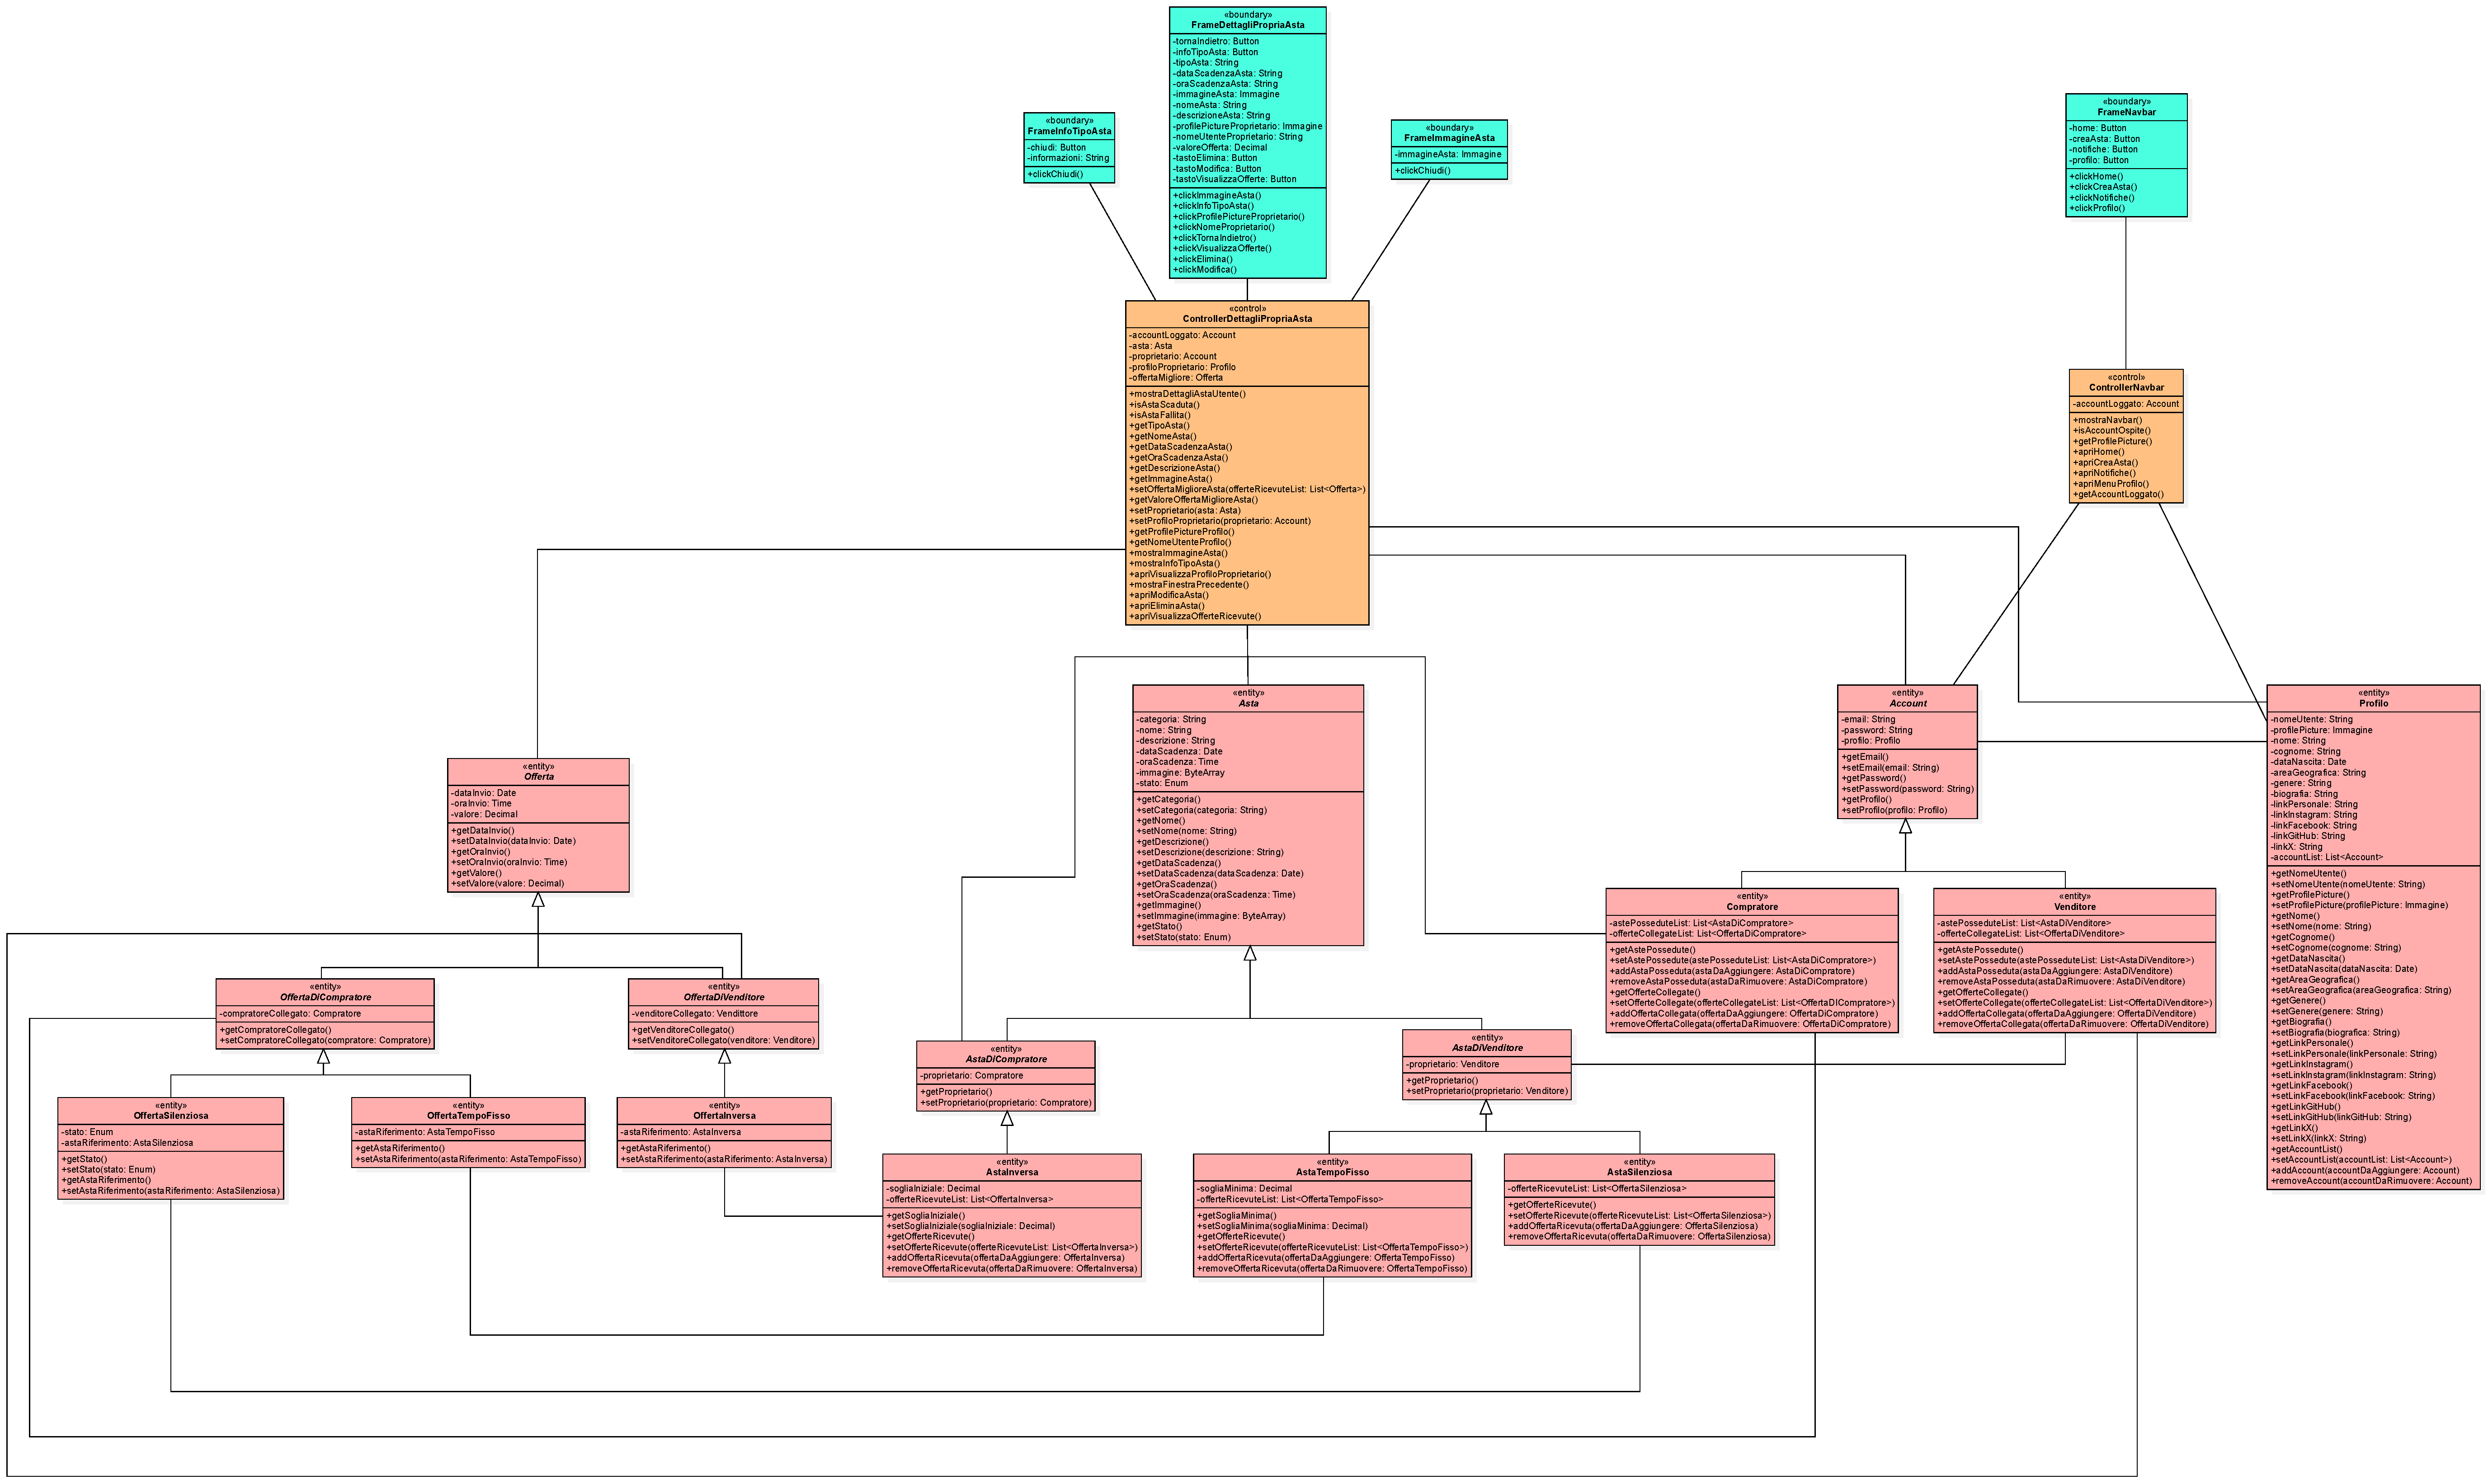
\includegraphics[width=1\linewidth]{Immagini/Diagrammi/Class Diagram/Analisi/Utente che ha effettuato l'accesso/VisualizzaDettagliPropriaAsta.pdf}
                \caption{Visualizza dettagli della propria asta}
            \end{figure}
            
            \begin{figure}[htbp!]
                \centering
                    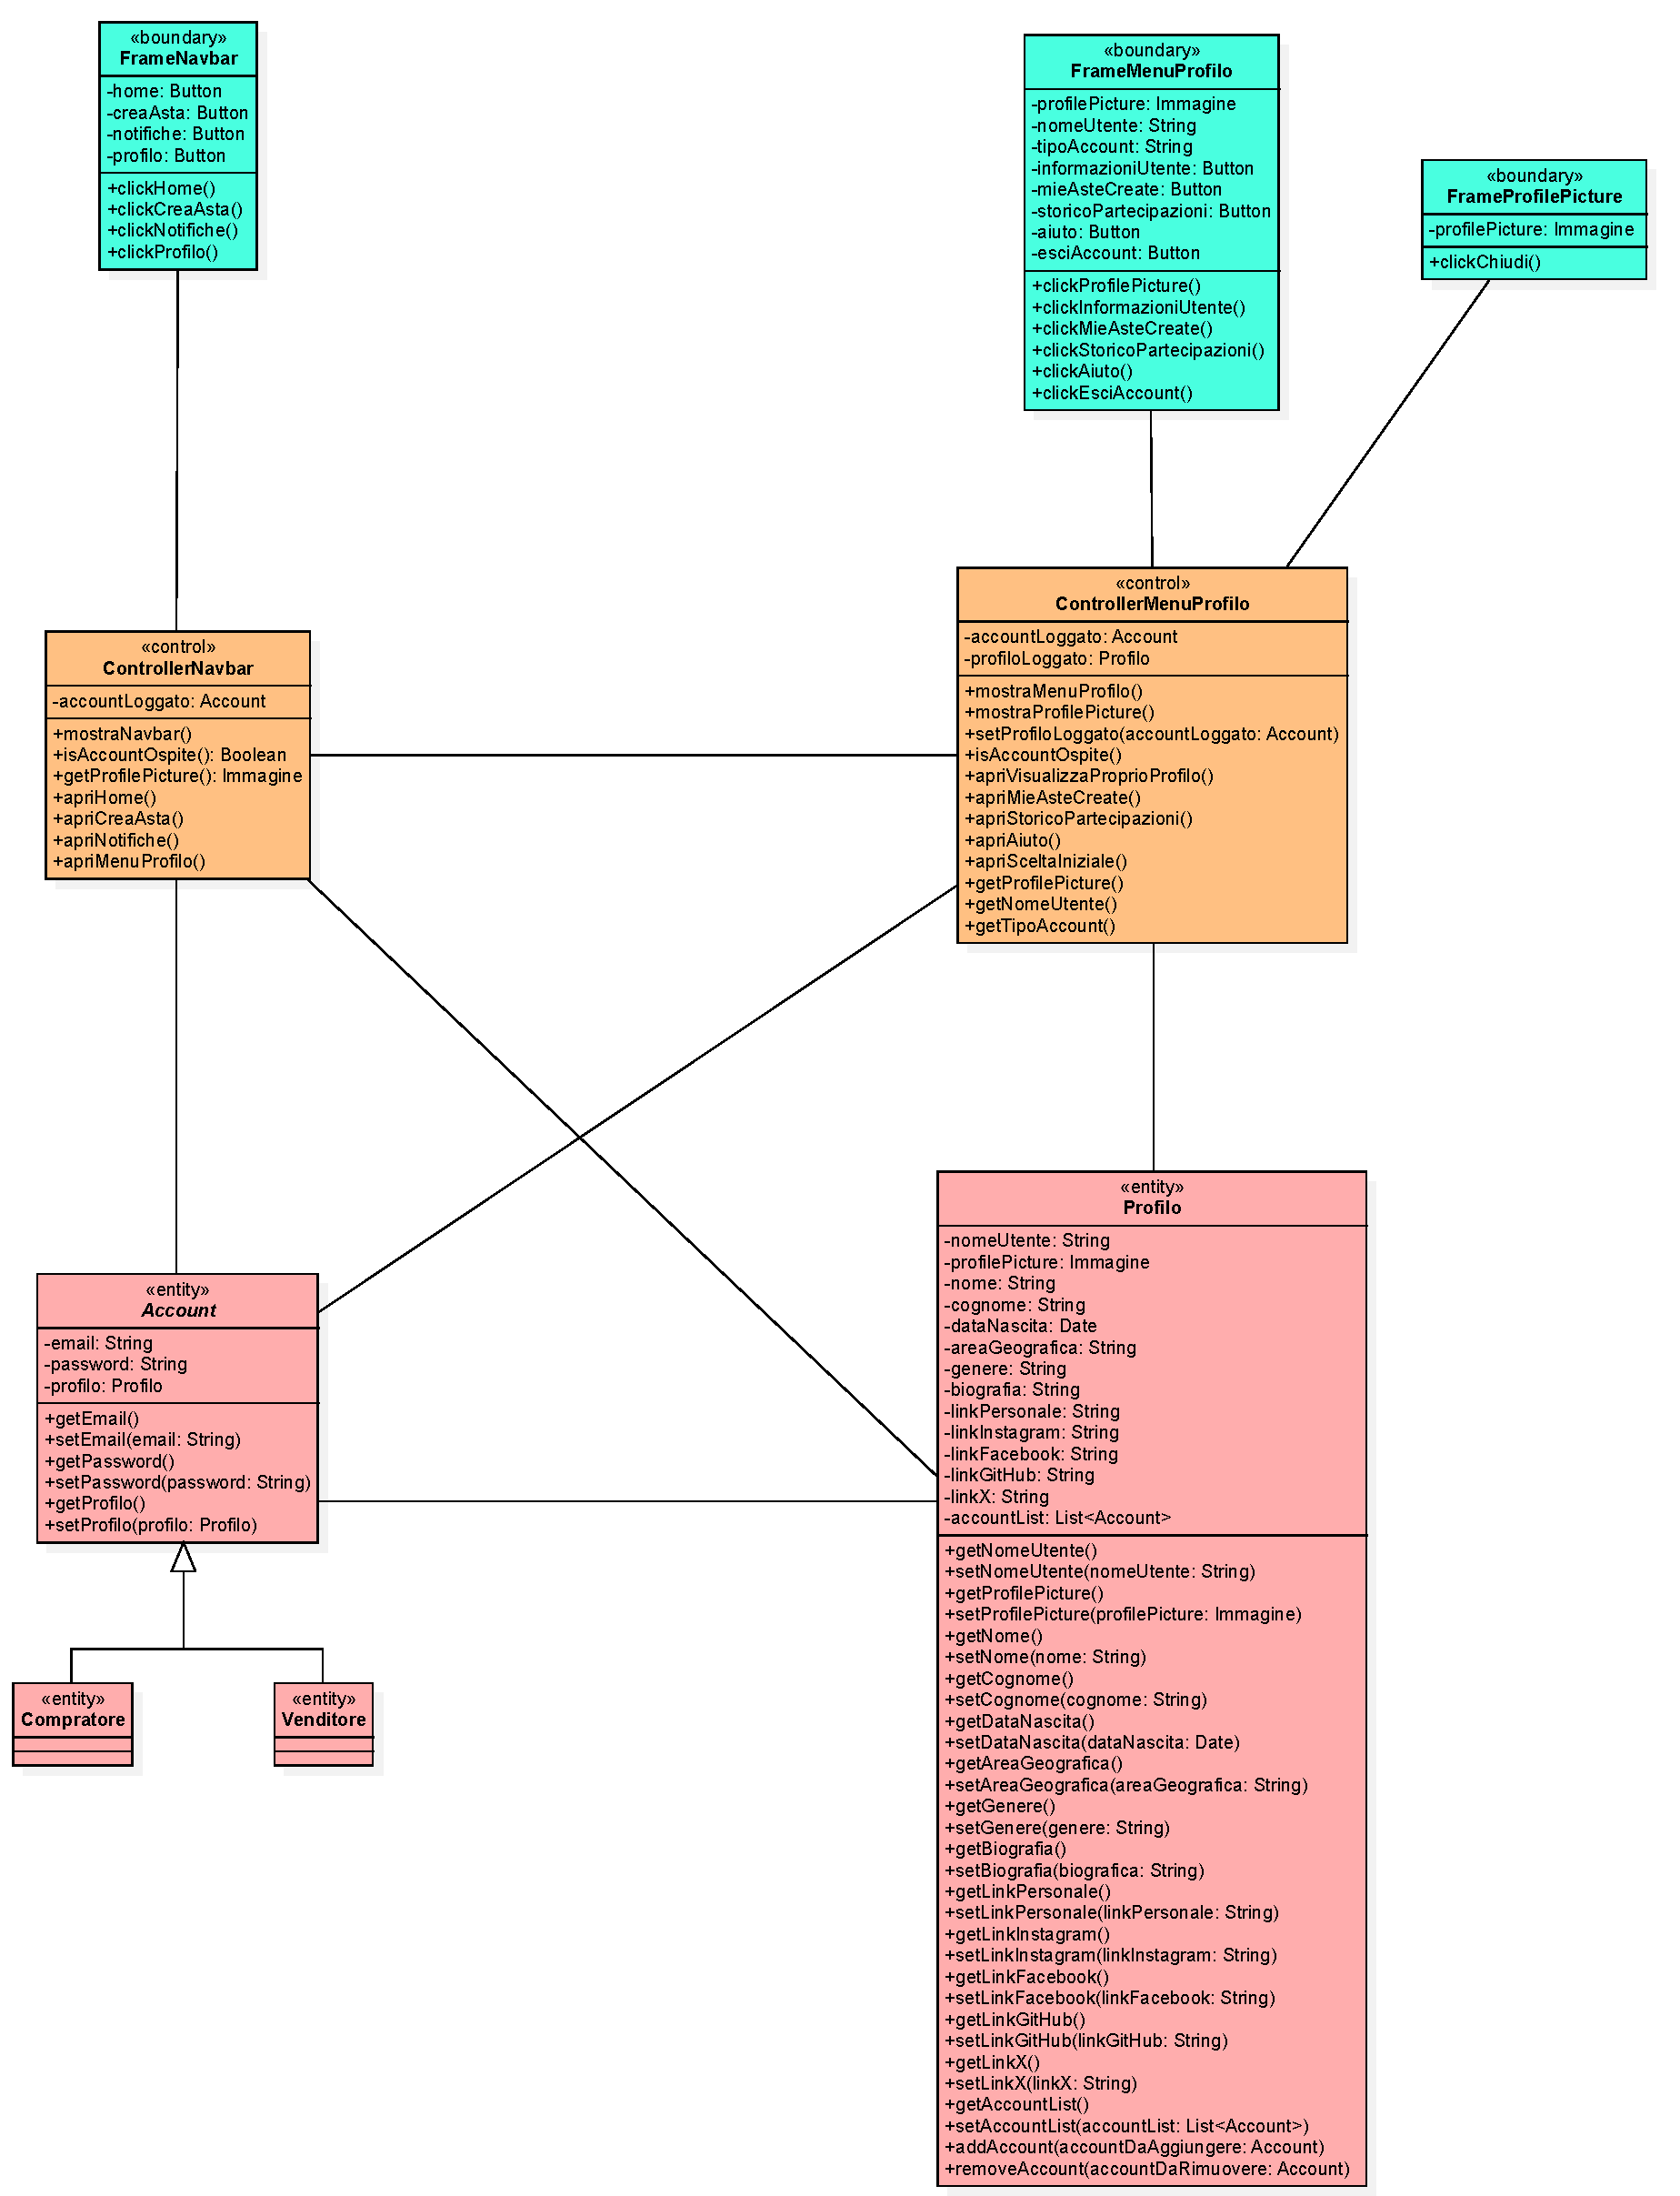
\includegraphics[width=1\linewidth]{Immagini/Diagrammi/Class Diagram/Analisi/Utente che ha effettuato l'accesso/VisualizzaMenuProfilo.pdf}
                \caption{Visualizza menu profilo}
            \end{figure}
            
            \begin{figure}[htbp!]
                \centering
                    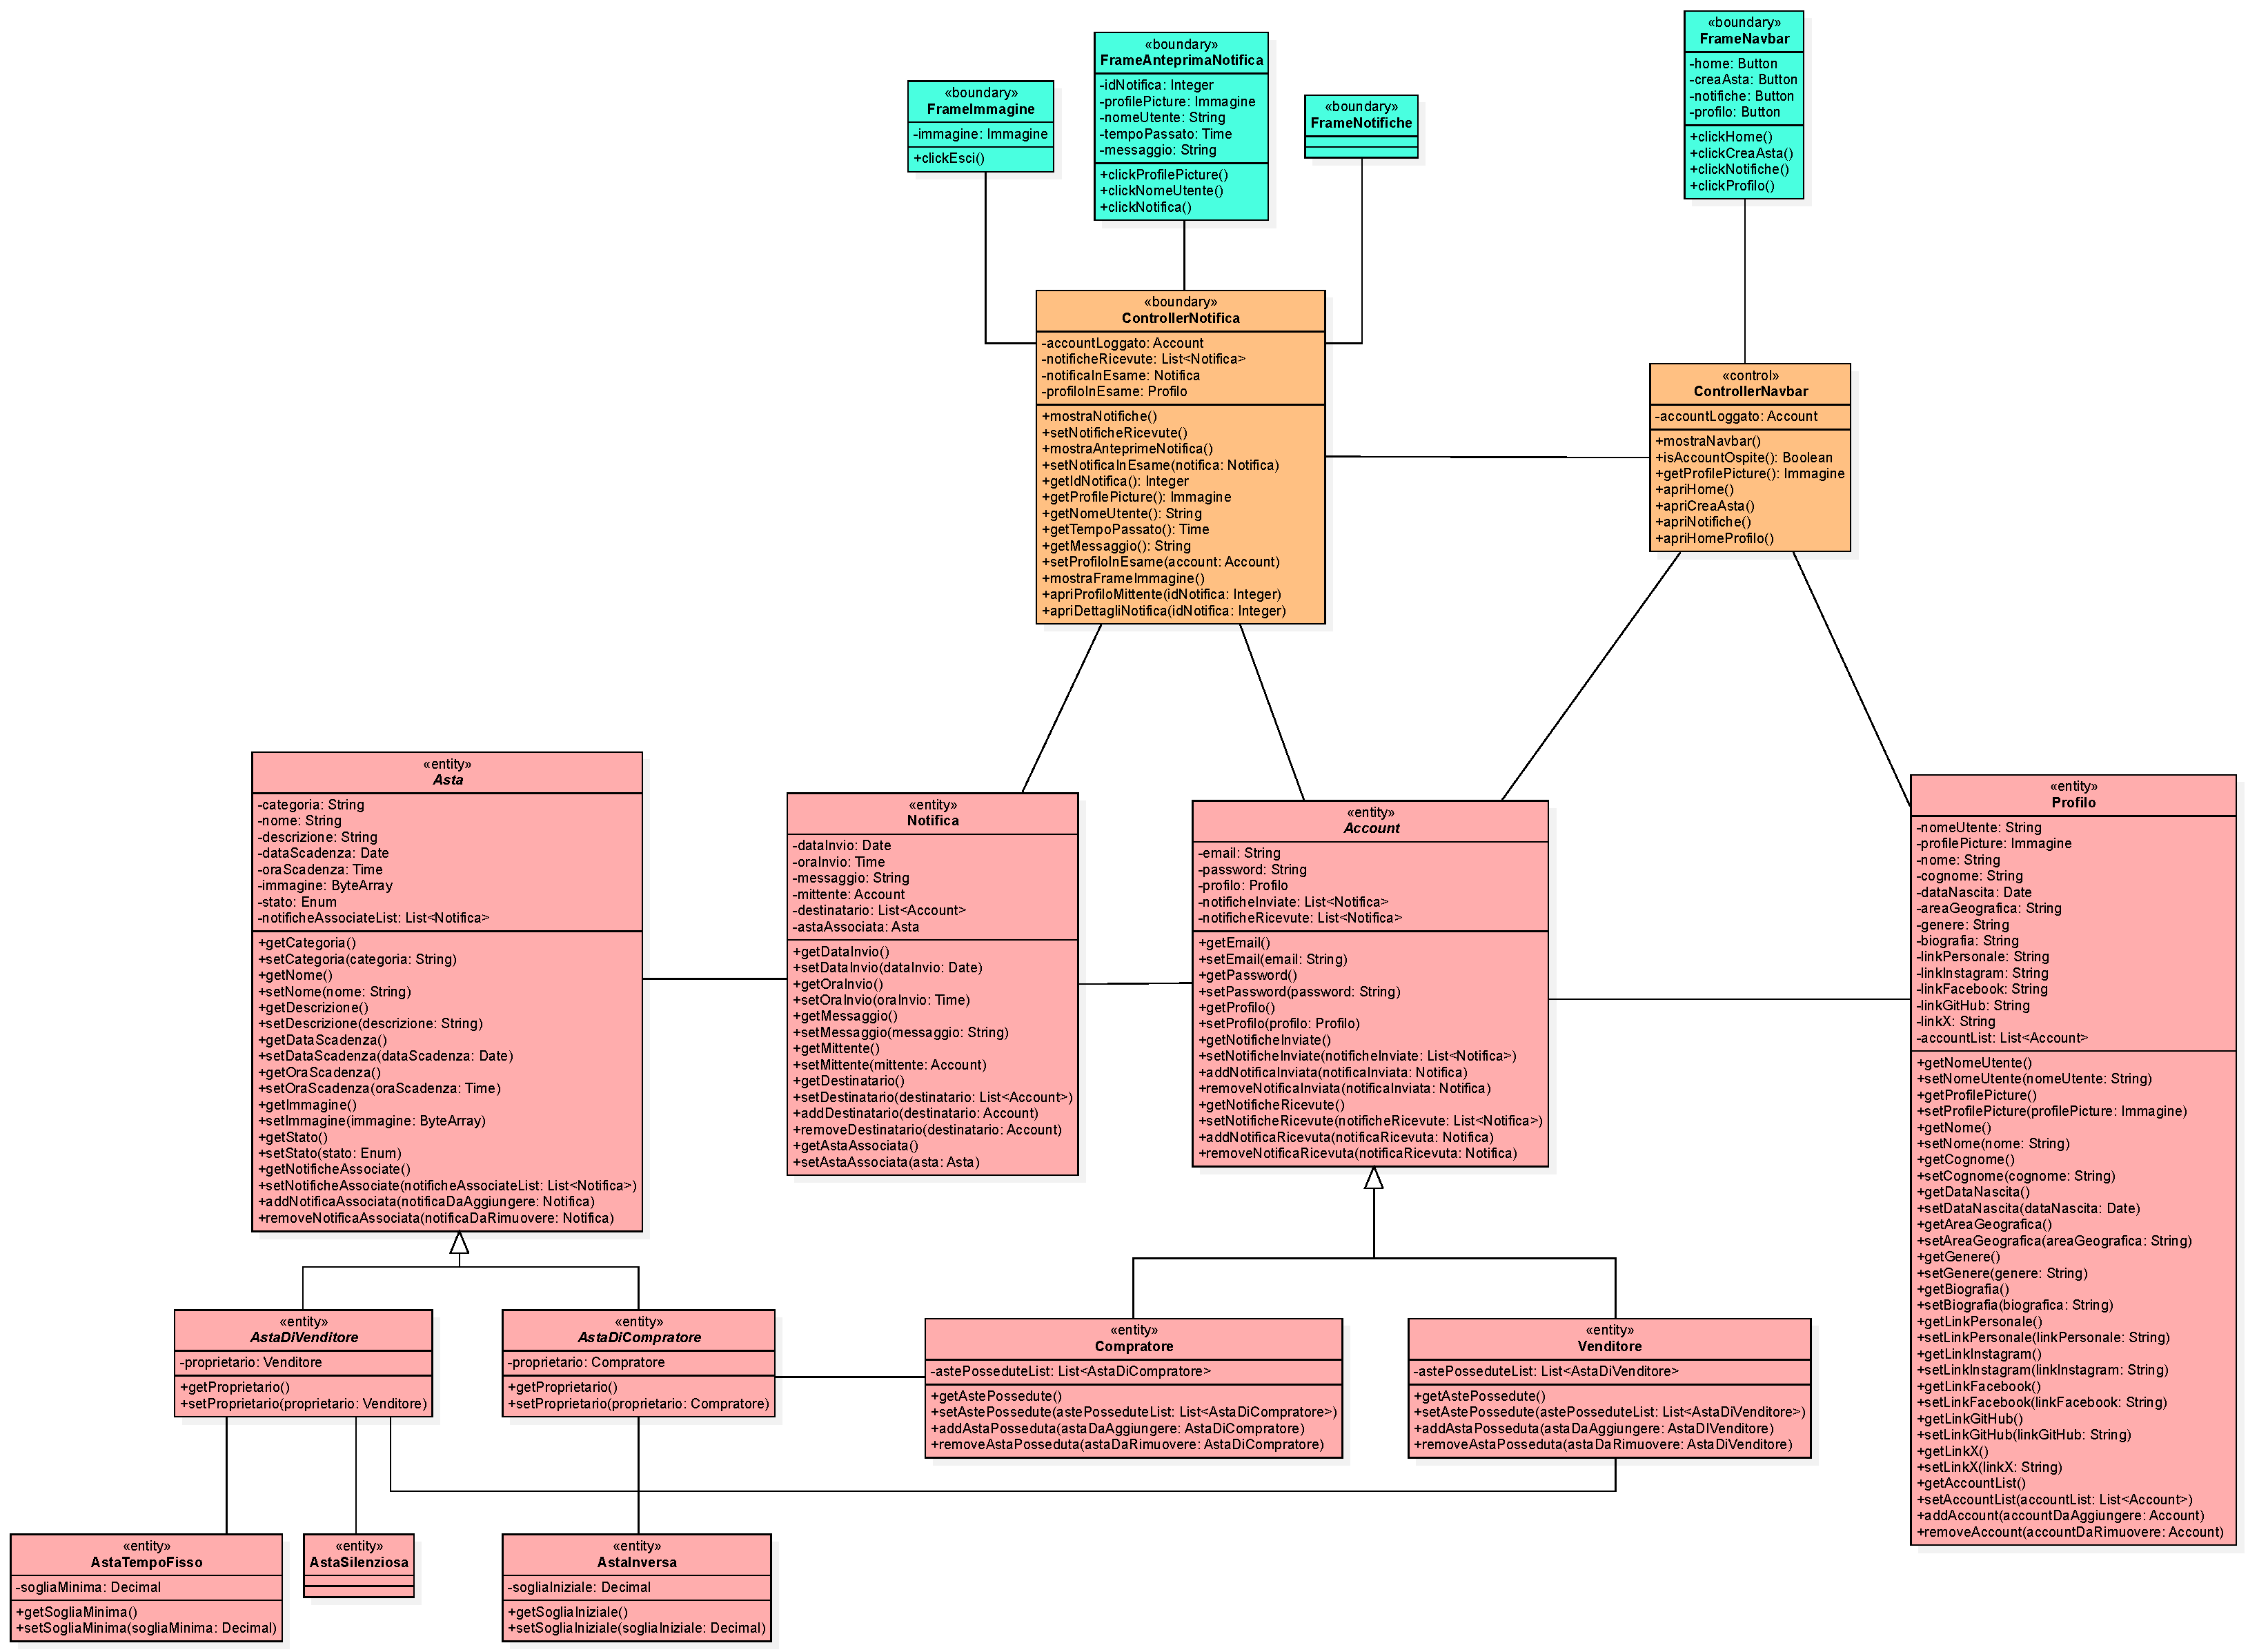
\includegraphics[width=1\linewidth]{Immagini/Diagrammi/Class Diagram/Analisi/Utente che ha effettuato l'accesso/VisualizzaNotifiche.pdf}
                \caption{Visualizza notifiche}
            \end{figure}
            
            \begin{figure}[htbp!]
                \centering
                    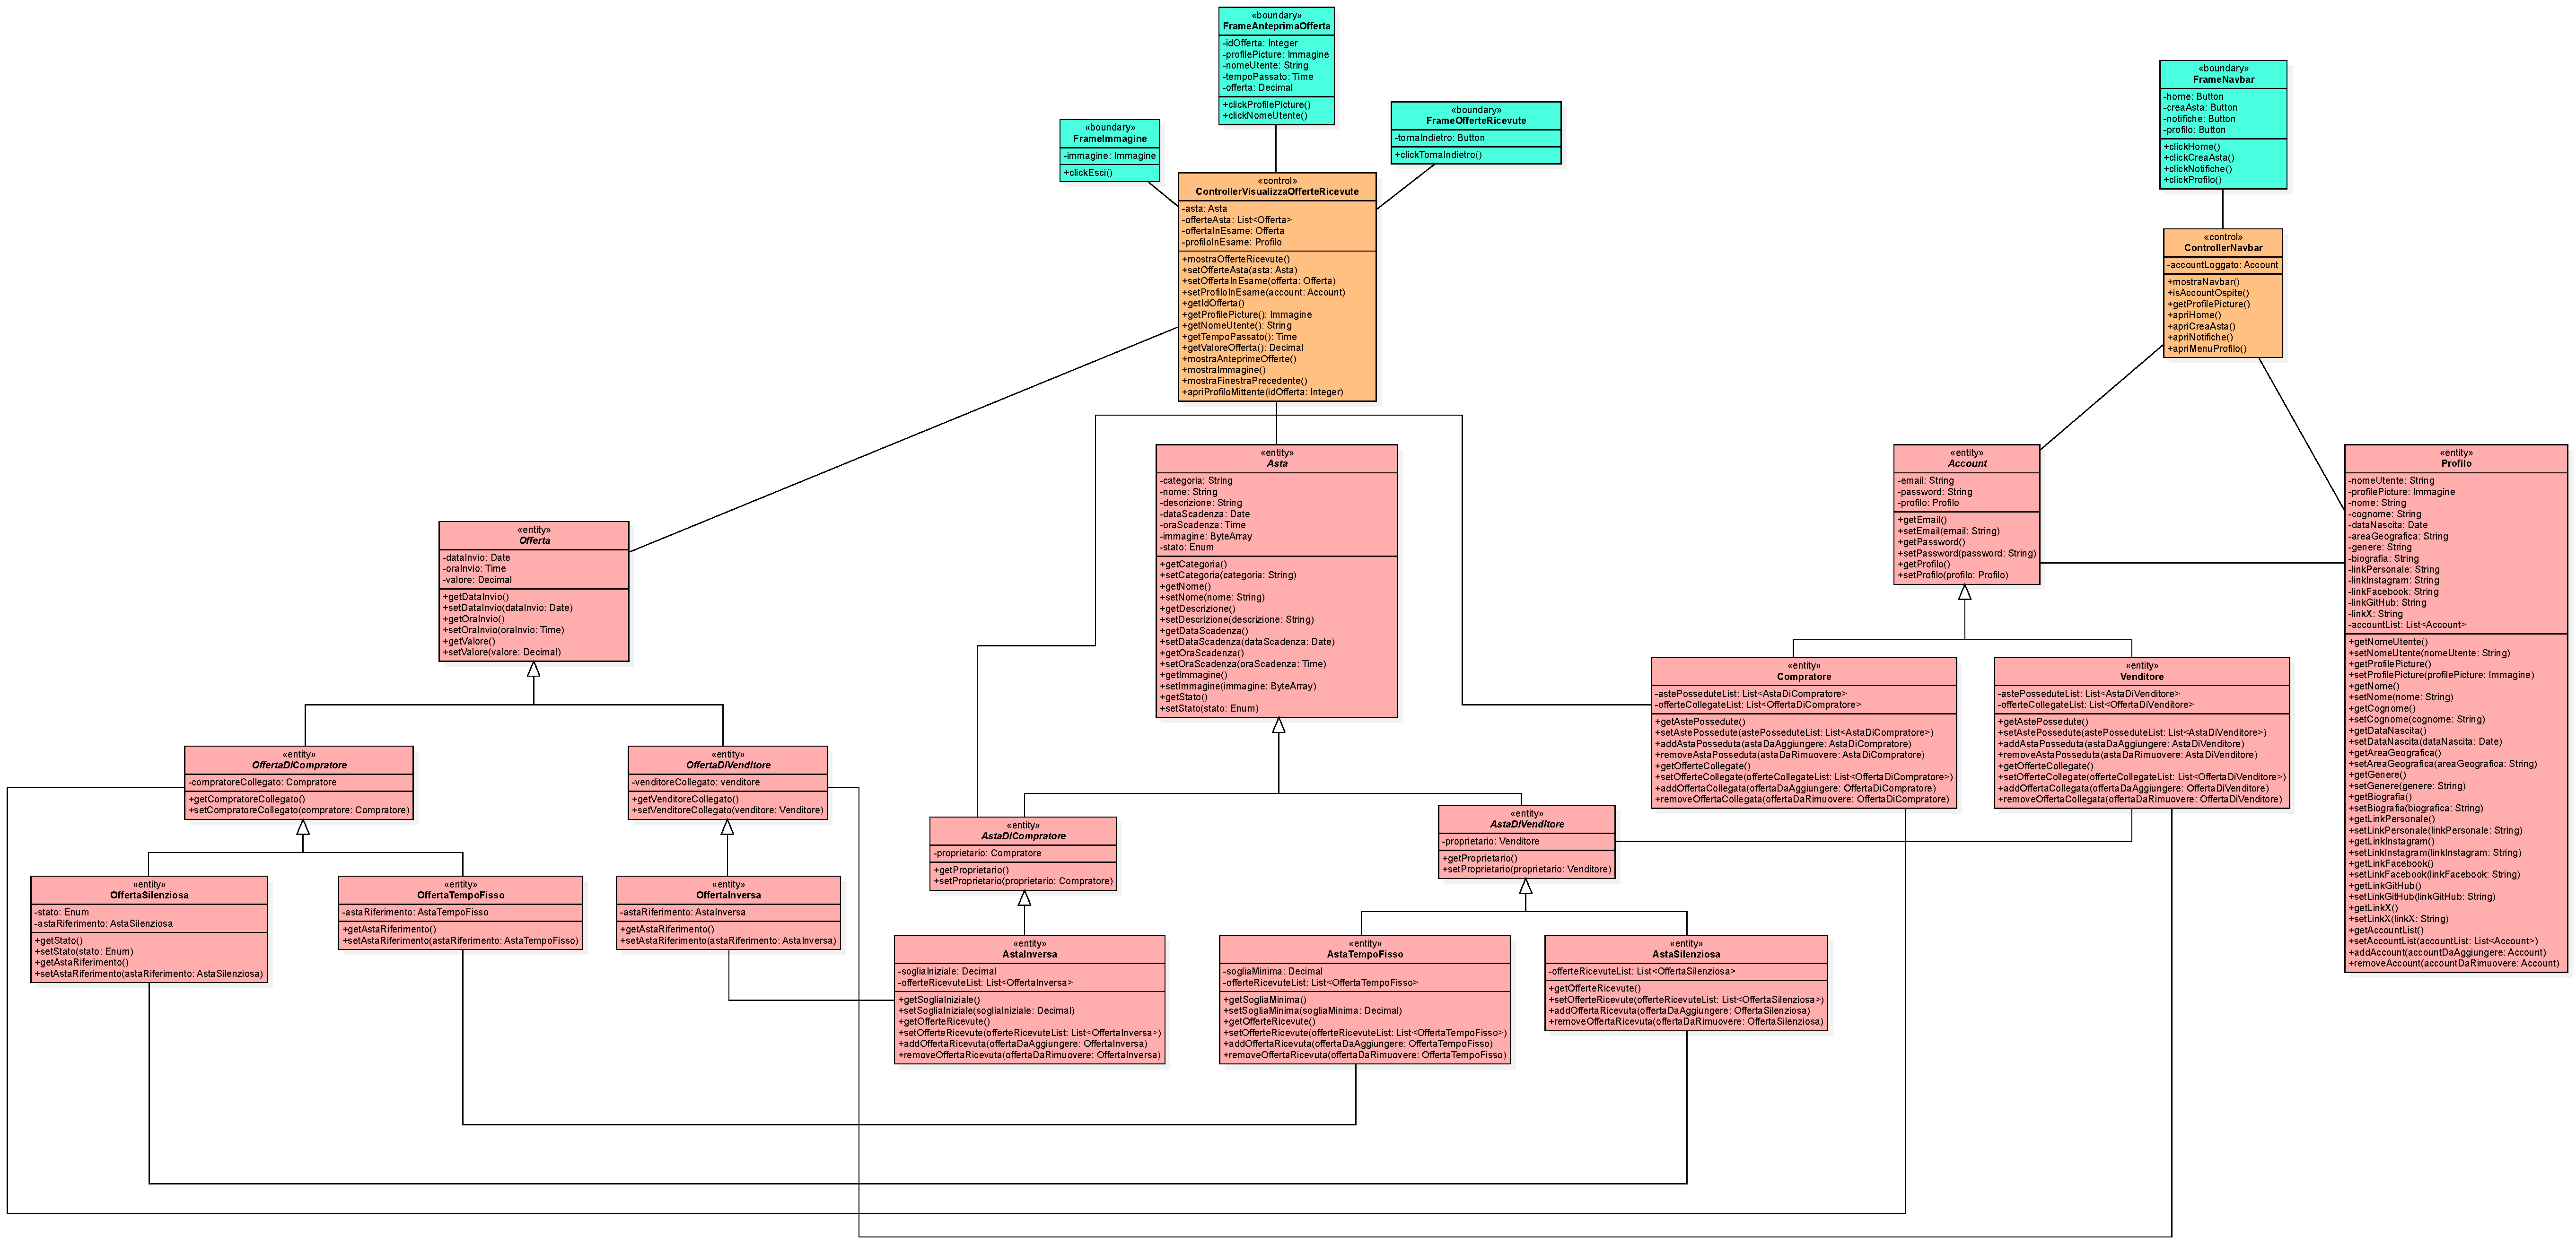
\includegraphics[width=1\linewidth]{Immagini/Diagrammi/Class Diagram/Analisi/Utente che ha effettuato l'accesso/VisualizzaOfferteRicevute.pdf}
                \caption{Visualizza offerte ricevute}
            \end{figure}
            
            \begin{figure}[htbp!]
                \centering
                    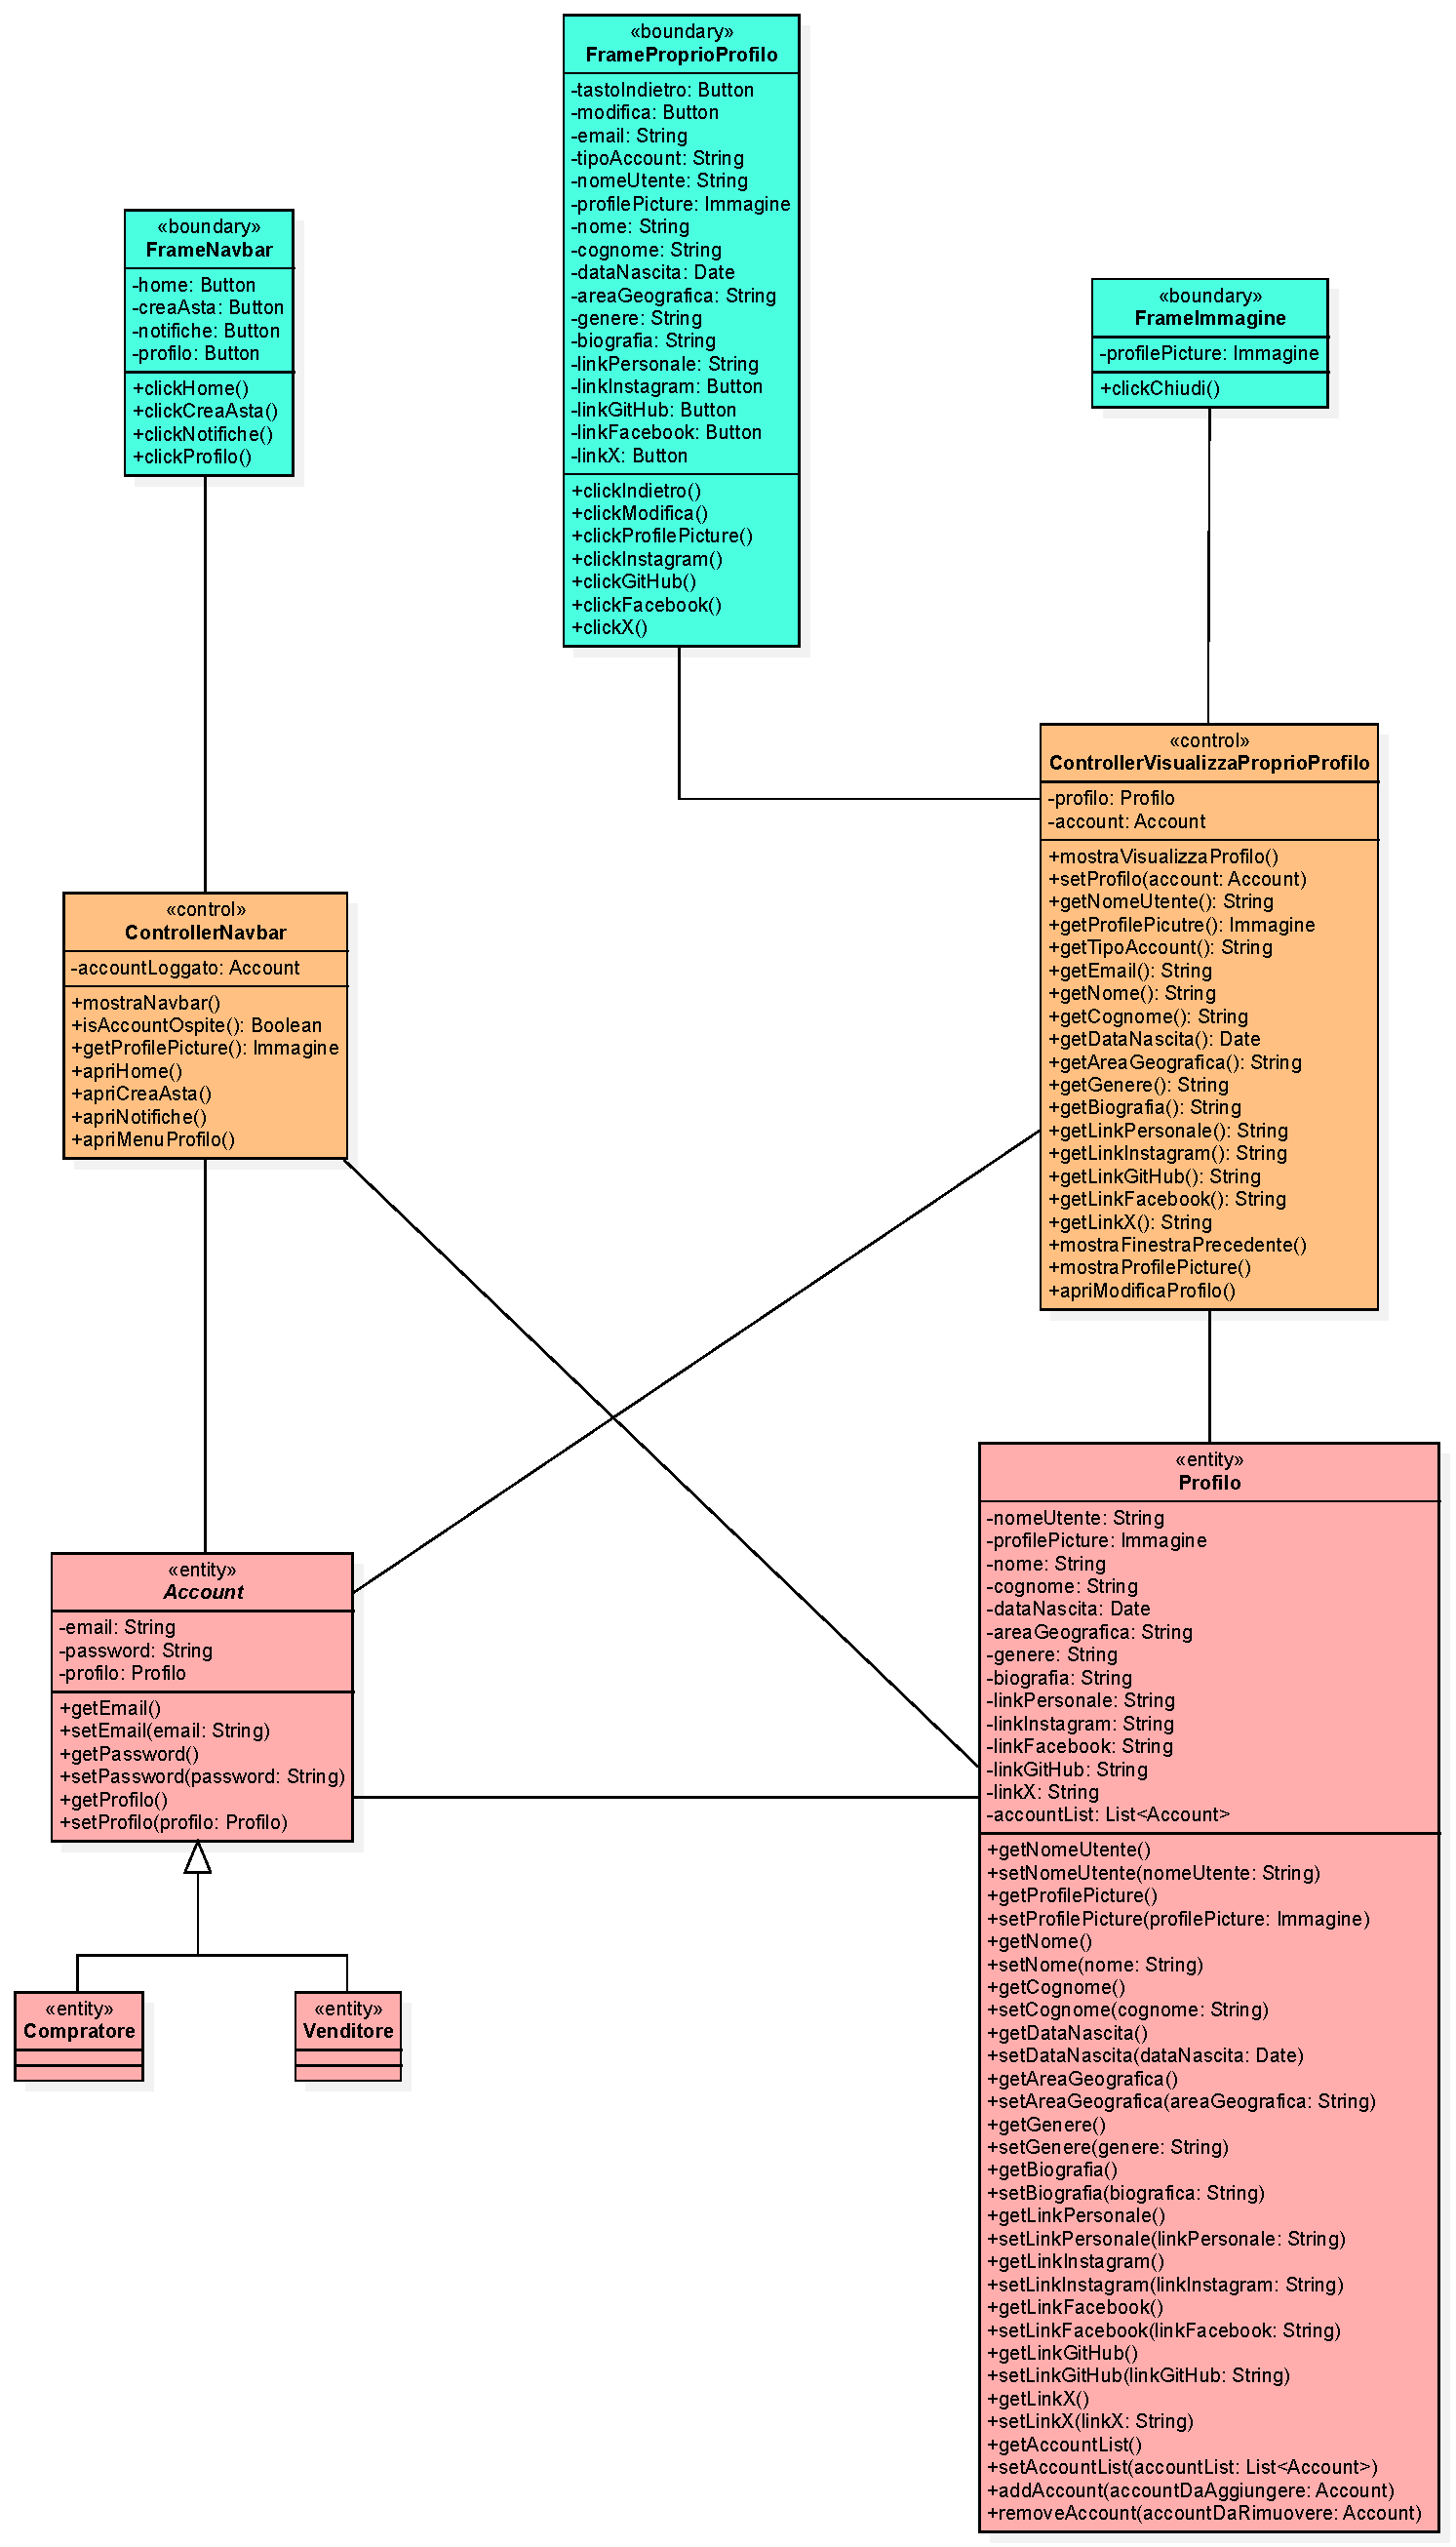
\includegraphics[width=0.75\linewidth]{Immagini/Diagrammi/Class Diagram/Analisi/Utente che ha effettuato l'accesso/VisualizzaProprioProfilo.pdf}
                \caption{Visualizza profilo personale}
            \end{figure}
            
            \begin{figure}[htbp!]
                \centering
                    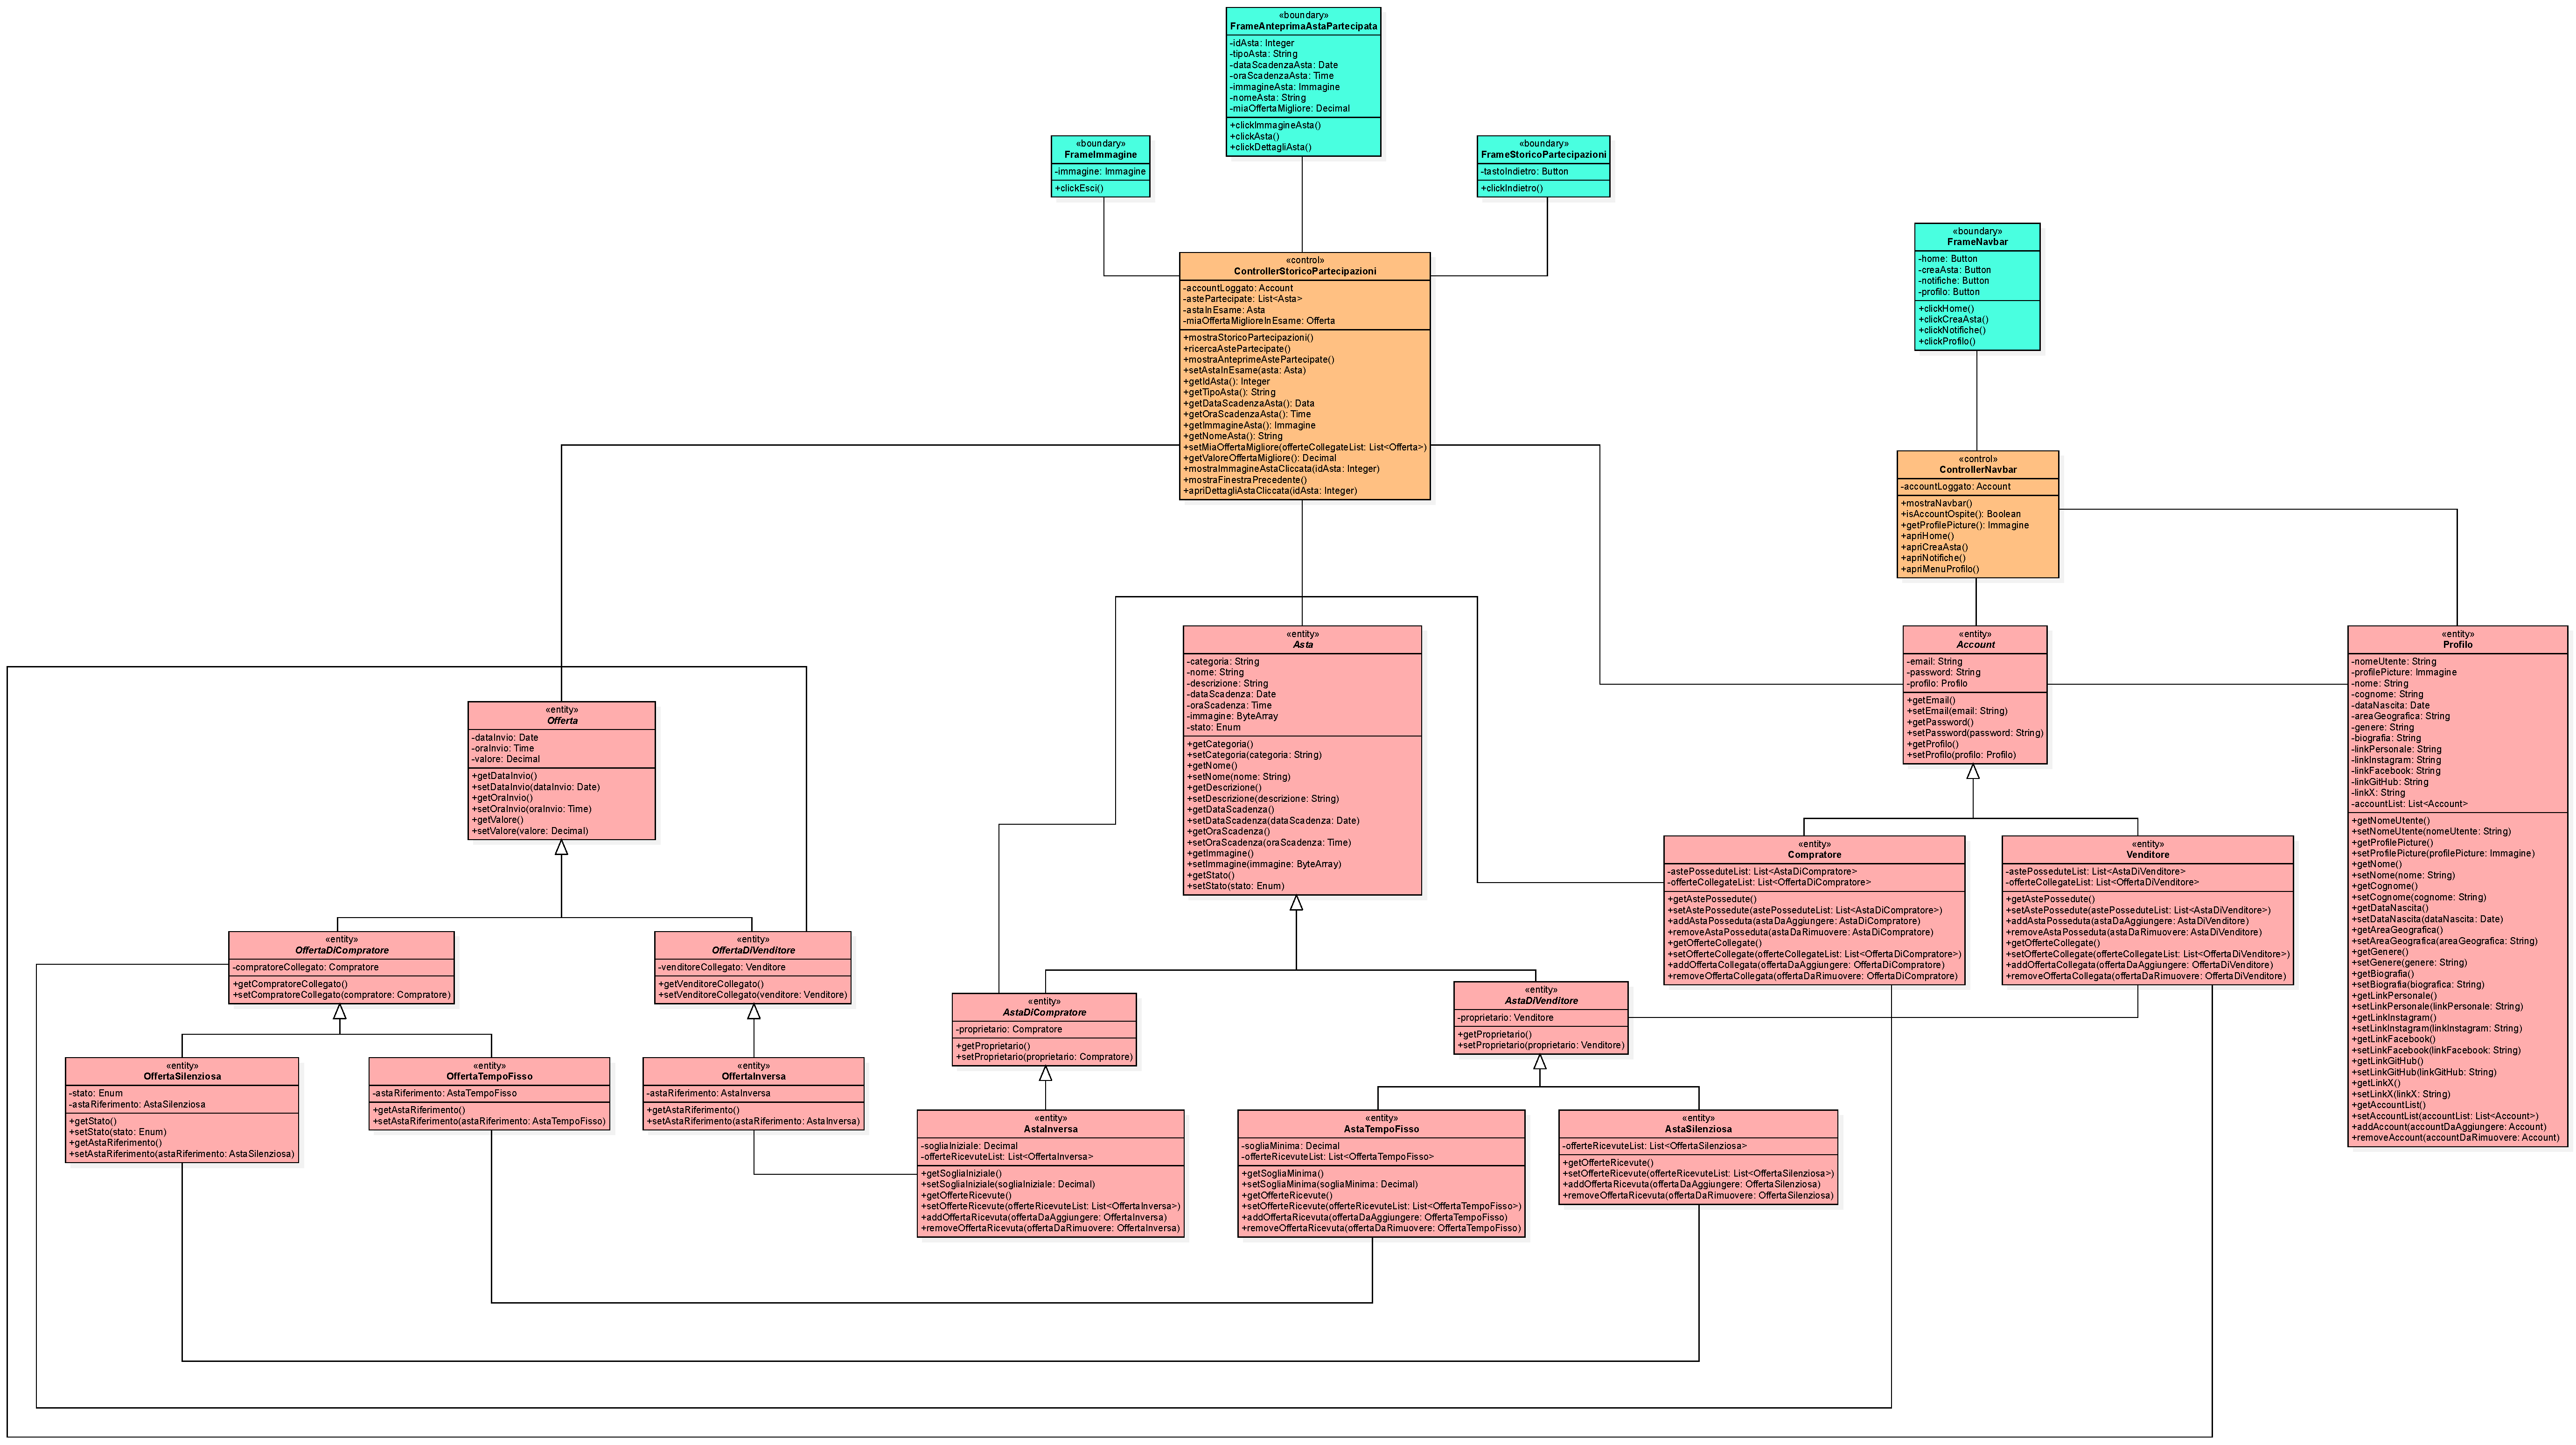
\includegraphics[width=1\linewidth]{Immagini/Diagrammi/Class Diagram/Analisi/Utente che ha effettuato l'accesso/VisualizzaStoricoPartecipazioni.pdf}
                \caption{Visualizza aste partecipate}
            \end{figure}
            
            \begin{figure}[htbp!]
                \centering
                    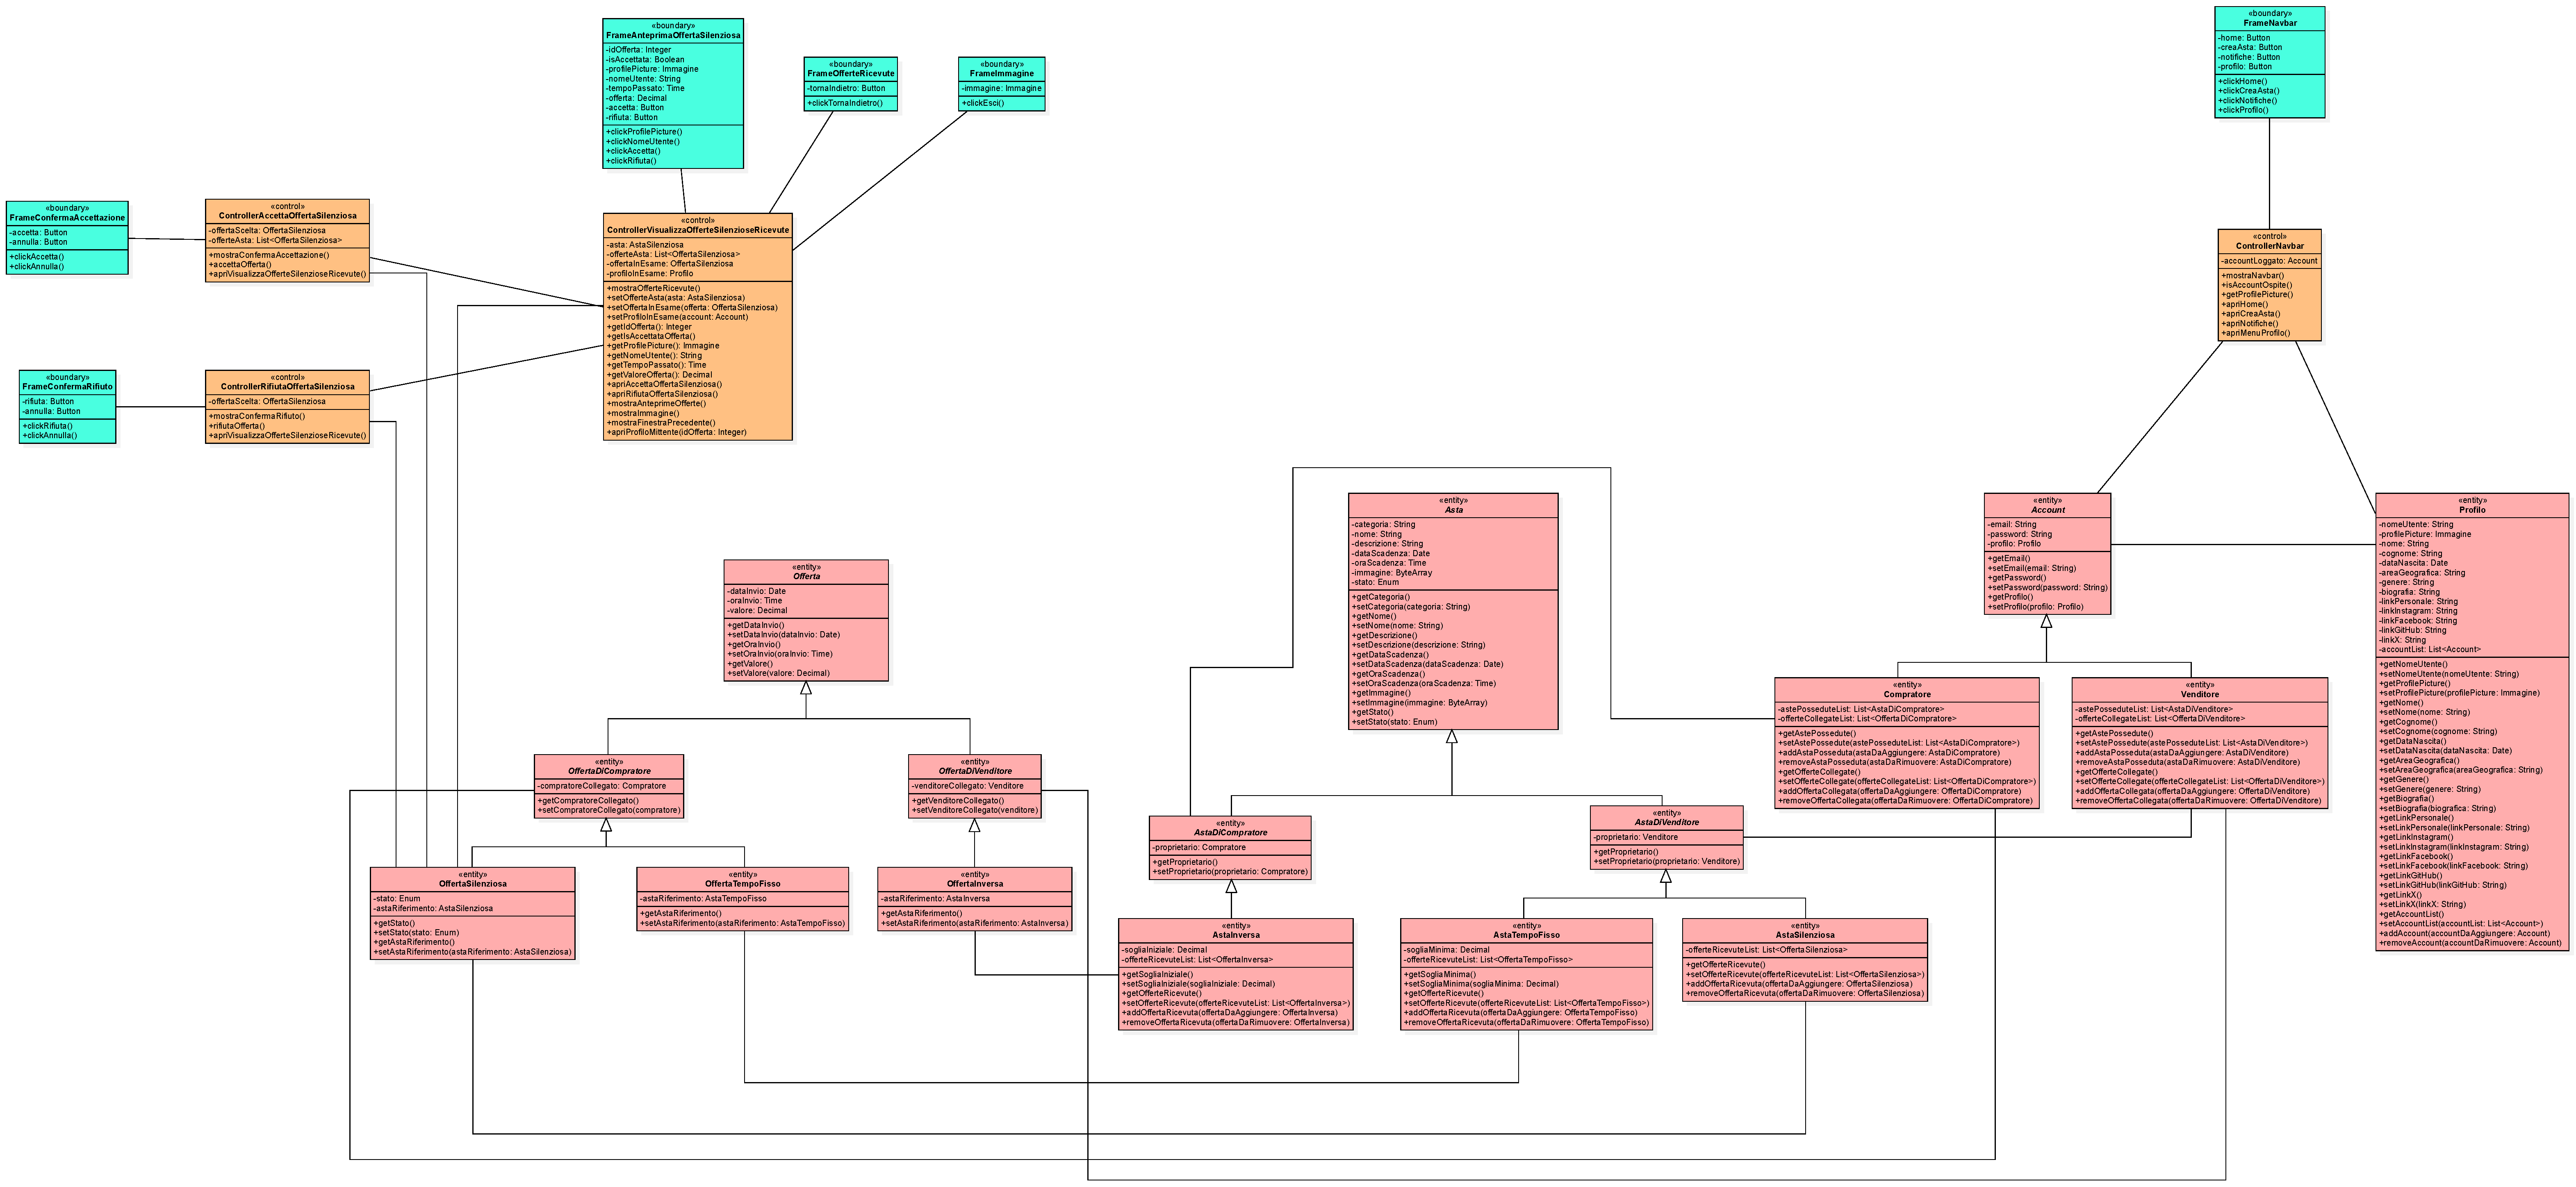
\includegraphics[width=1\linewidth]{Immagini/Diagrammi/Class Diagram/Analisi/Venditore e compratore/AccettaRifiutaOffertaSilenziosa.pdf}
                \caption{Accetta o rifiuta un'offerta per un'asta silenziosa}
            \end{figure}
            
            \begin{figure}[htbp!]
                \centering
                    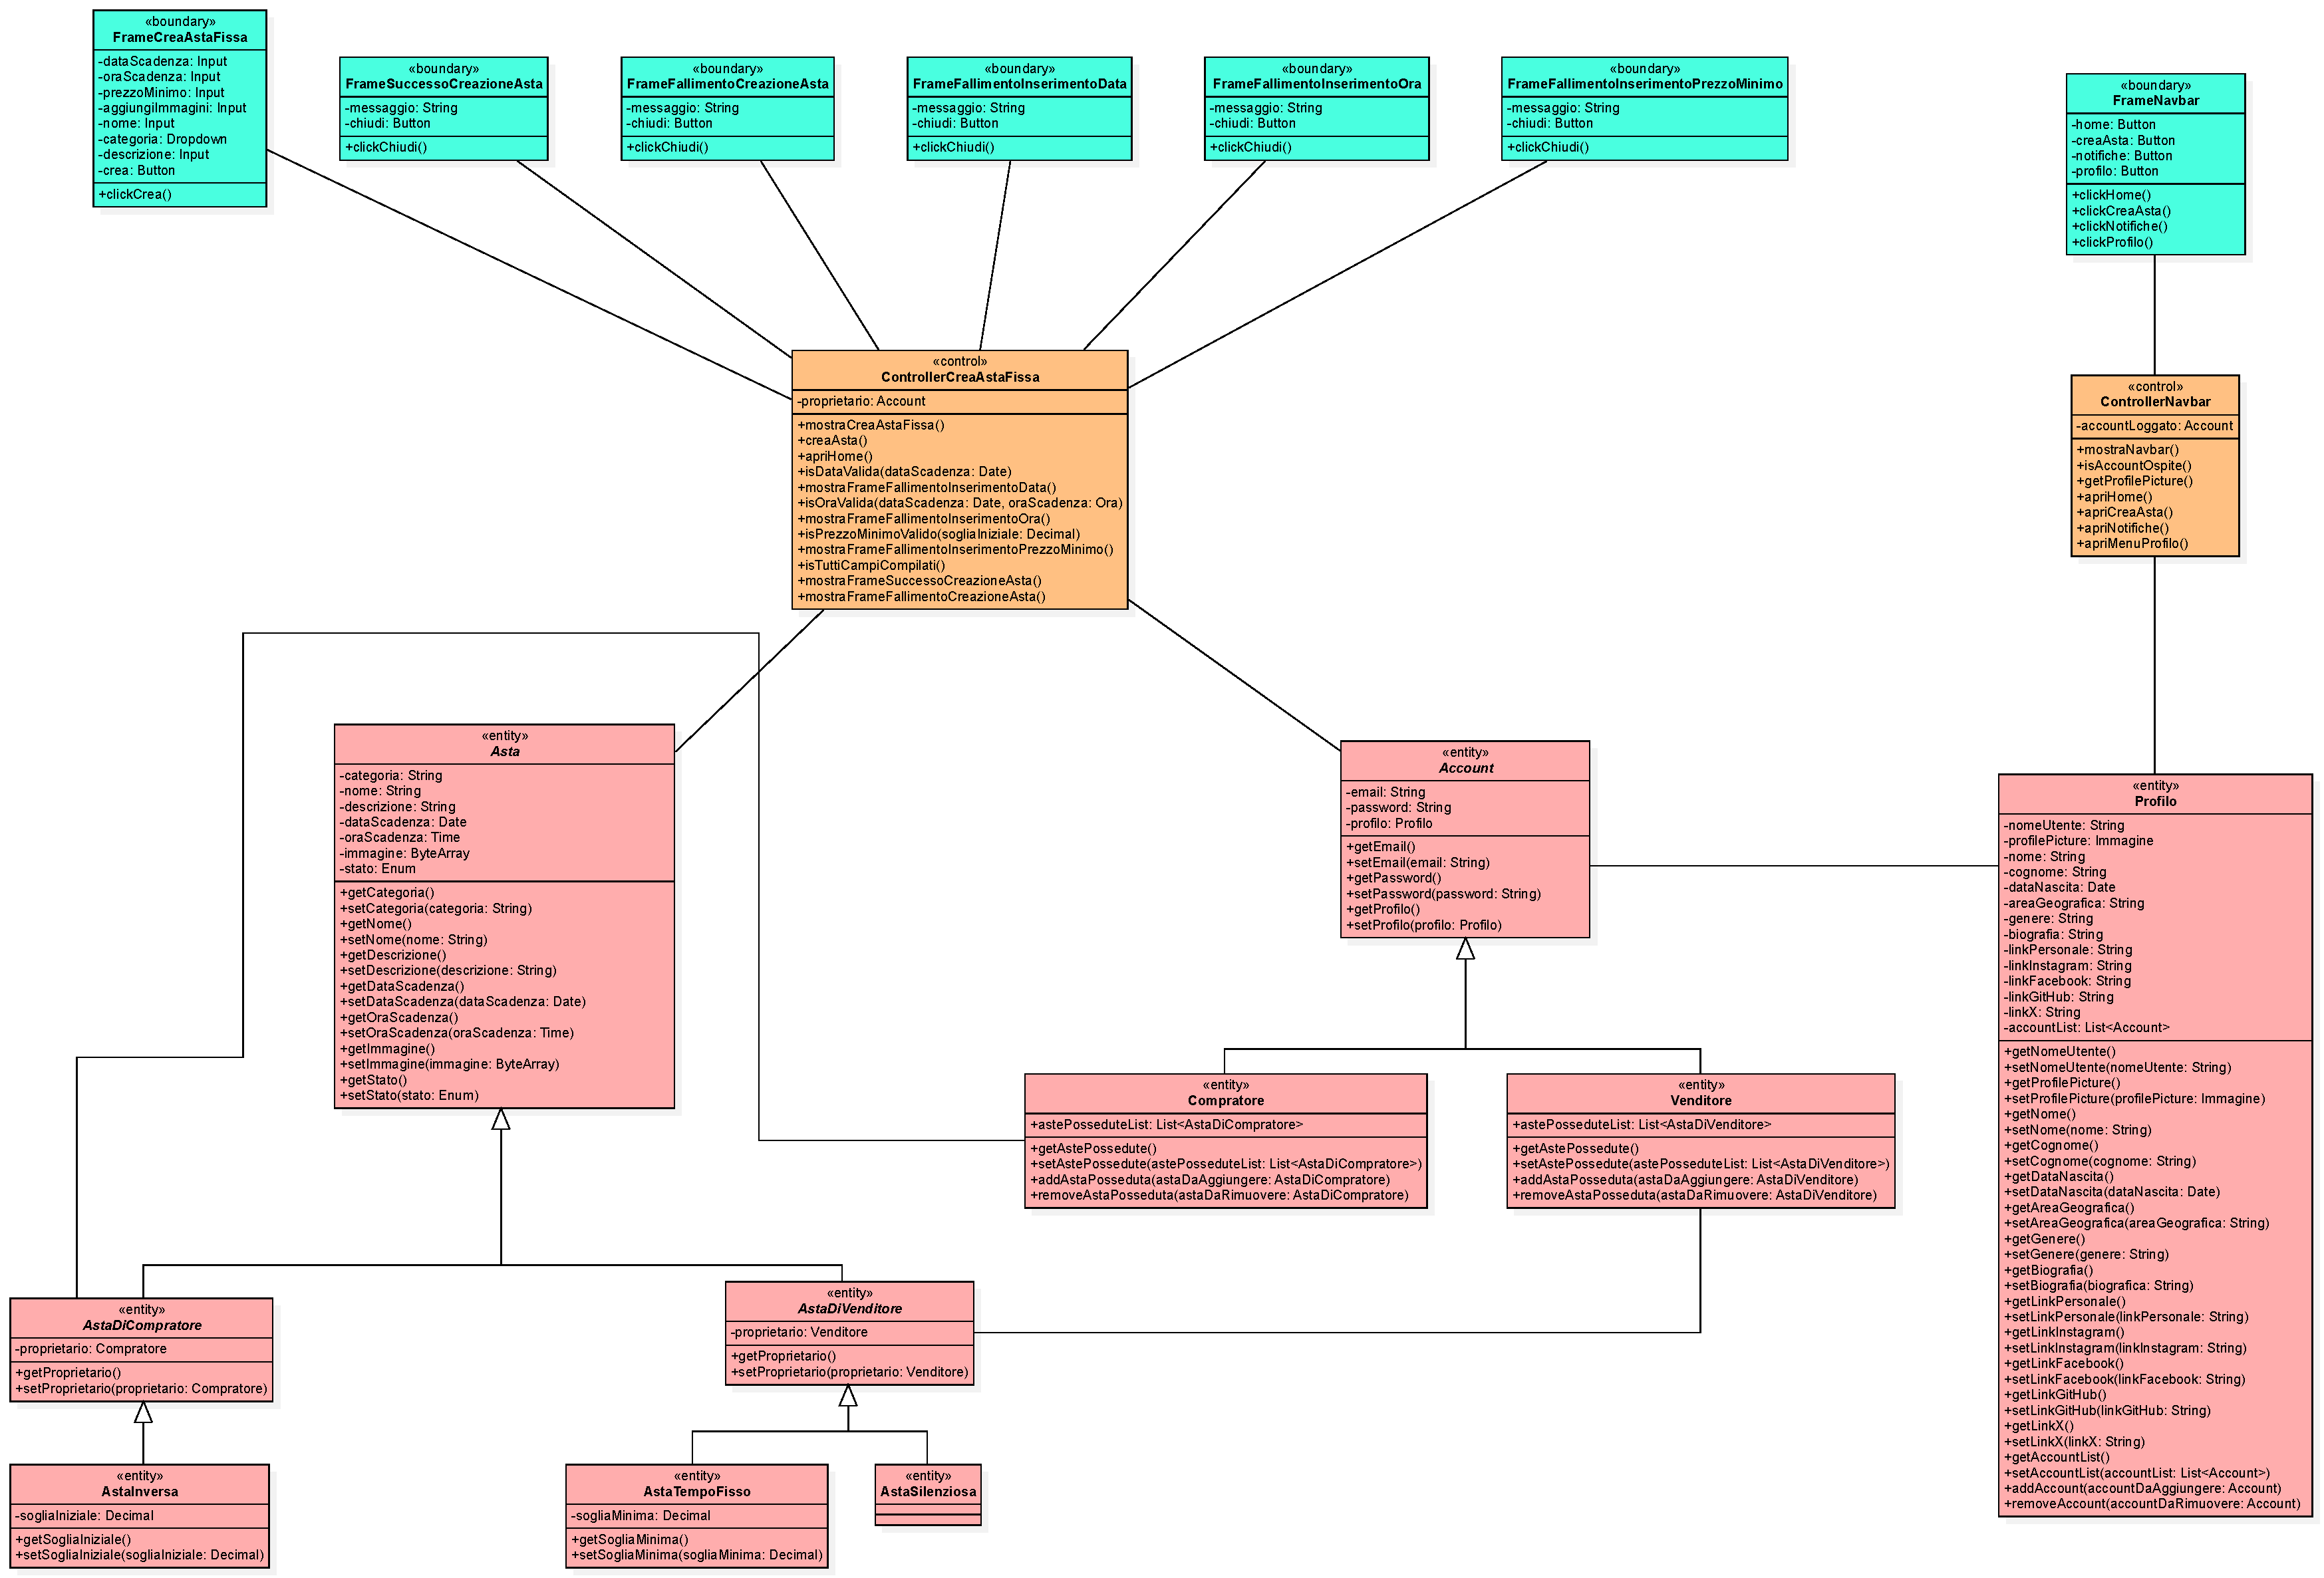
\includegraphics[width=1\linewidth]{Immagini/Diagrammi/Class Diagram/Analisi/Venditore e compratore/CreaAstaFissa.pdf}
                \caption{Crea un'asta a tempo fisso}
            \end{figure}
            
            \begin{figure}[htbp!]
                \centering
                    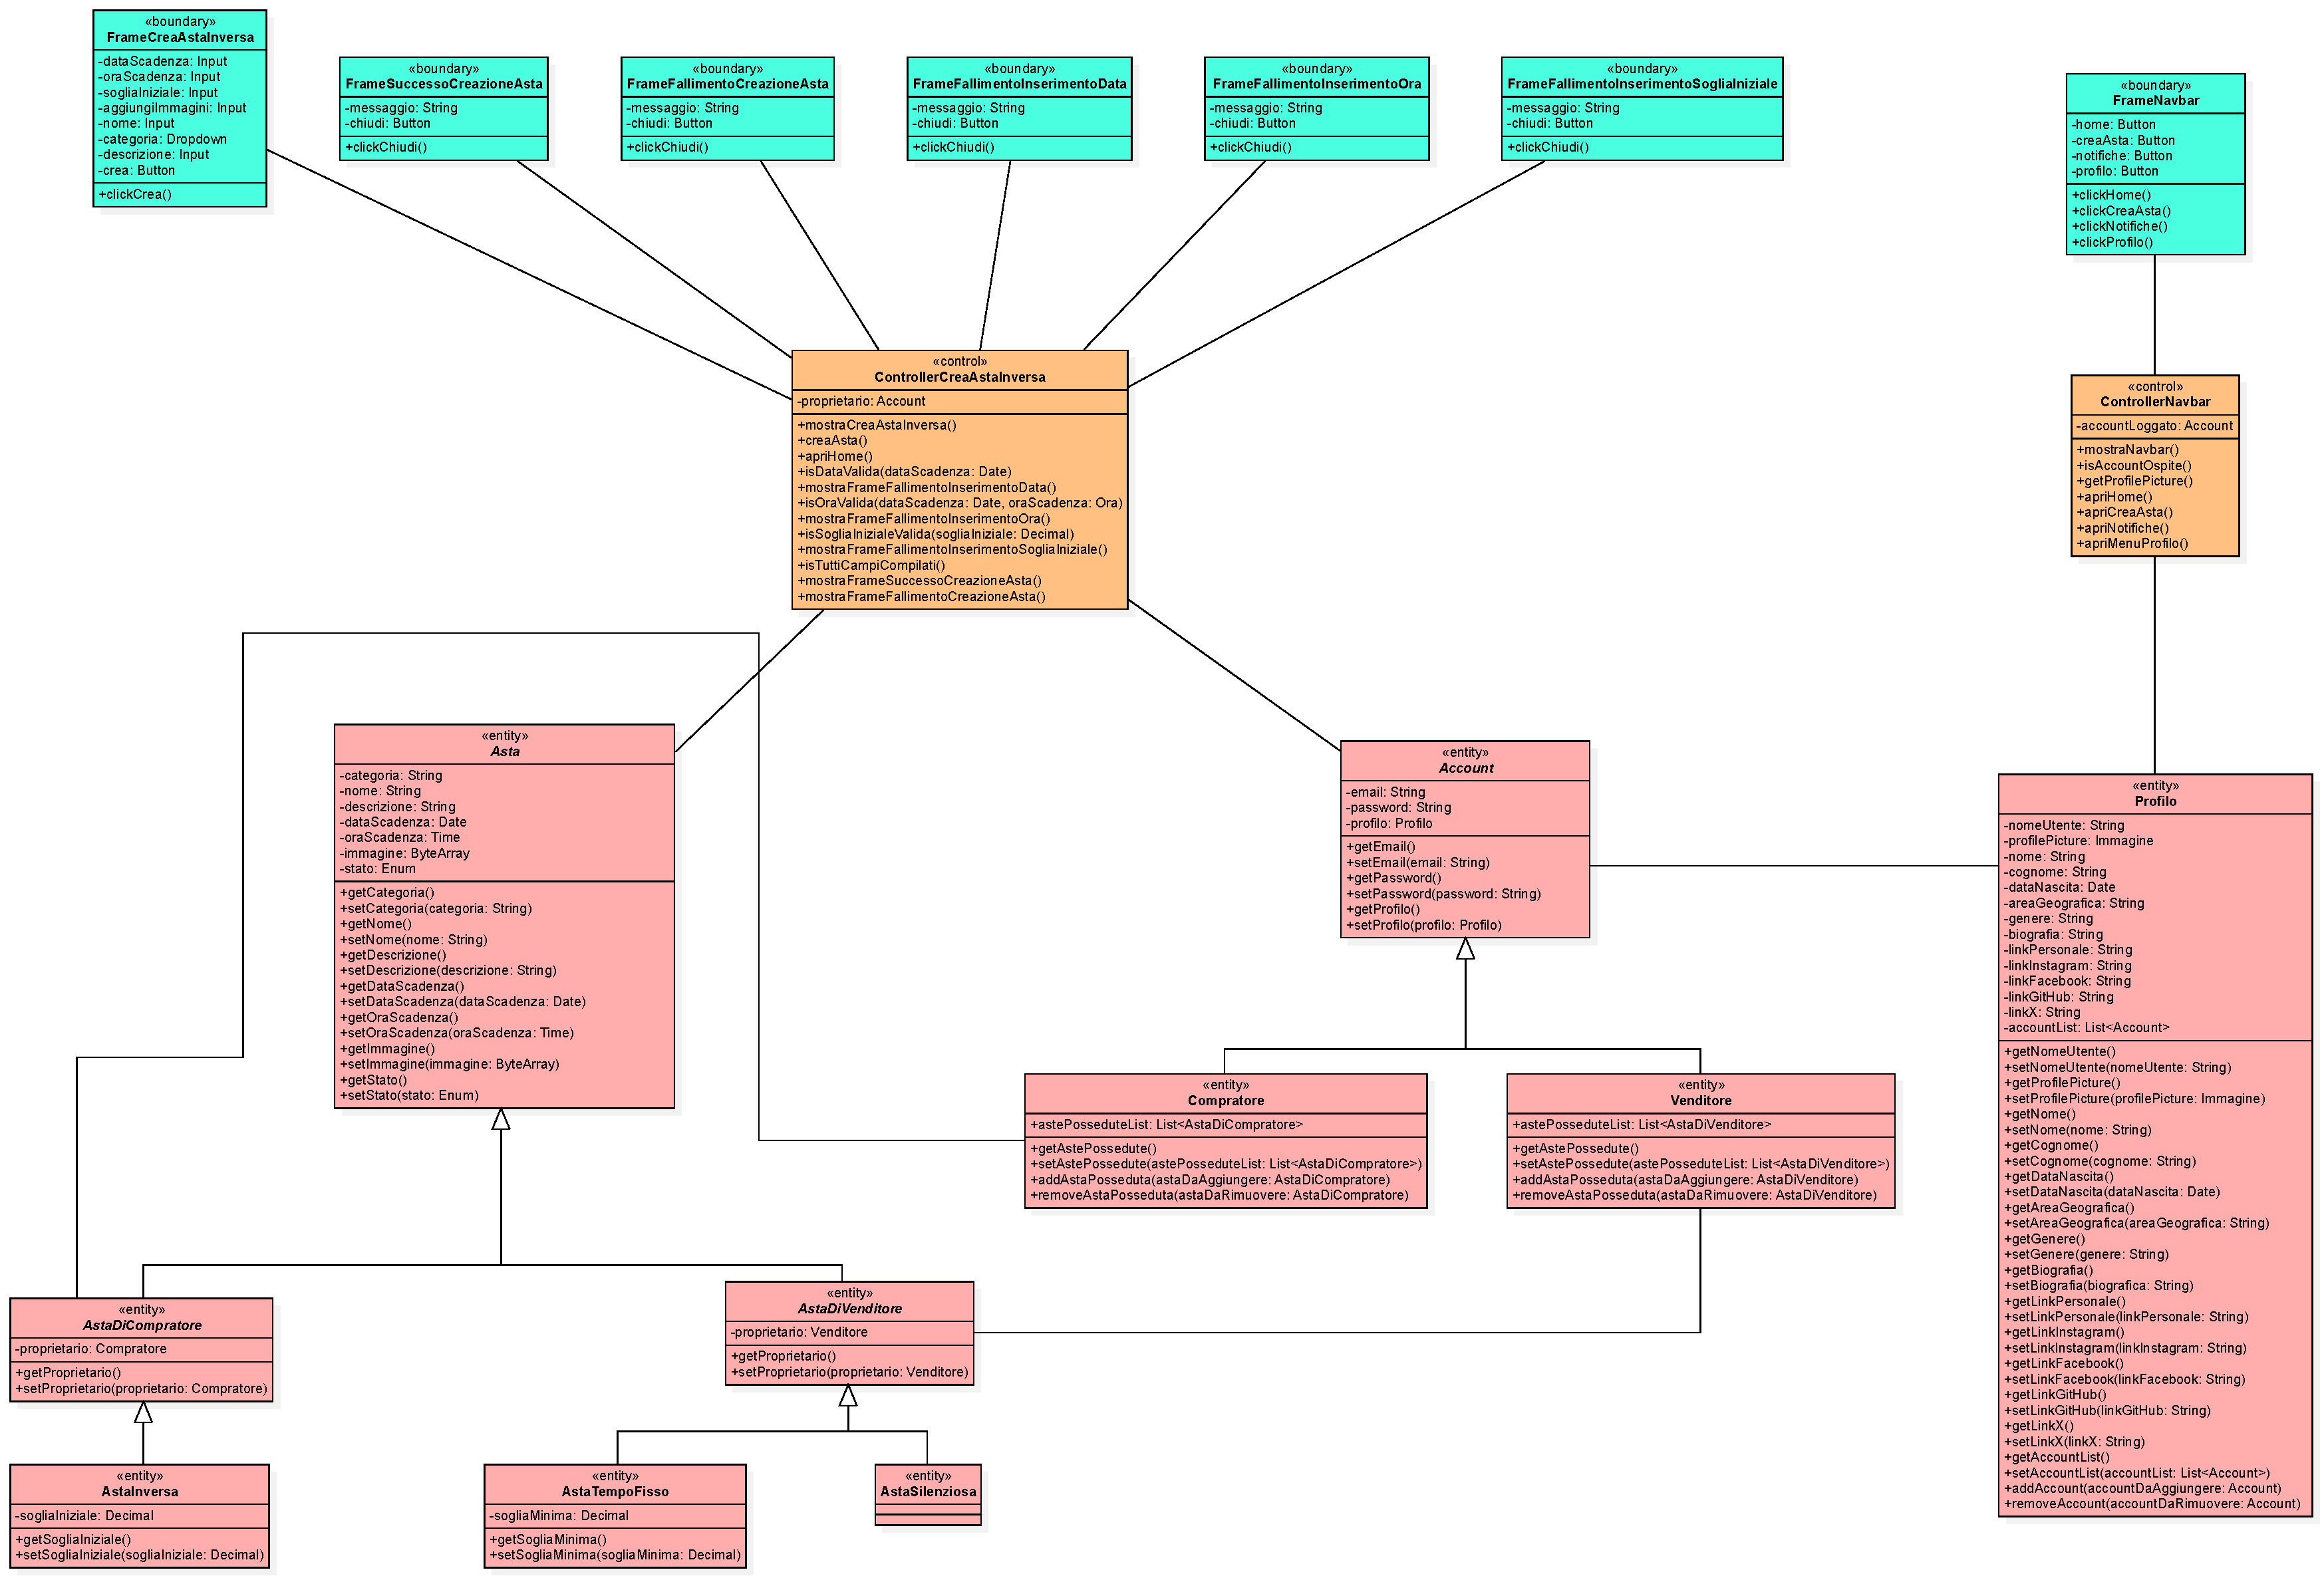
\includegraphics[width=1\linewidth]{Immagini/Diagrammi/Class Diagram/Analisi/Venditore e compratore/CreaAstaInversa.pdf}
                \caption{Crea un'asta inversa}
            \end{figure}
            
            \begin{figure}[htbp!]
                \centering
                    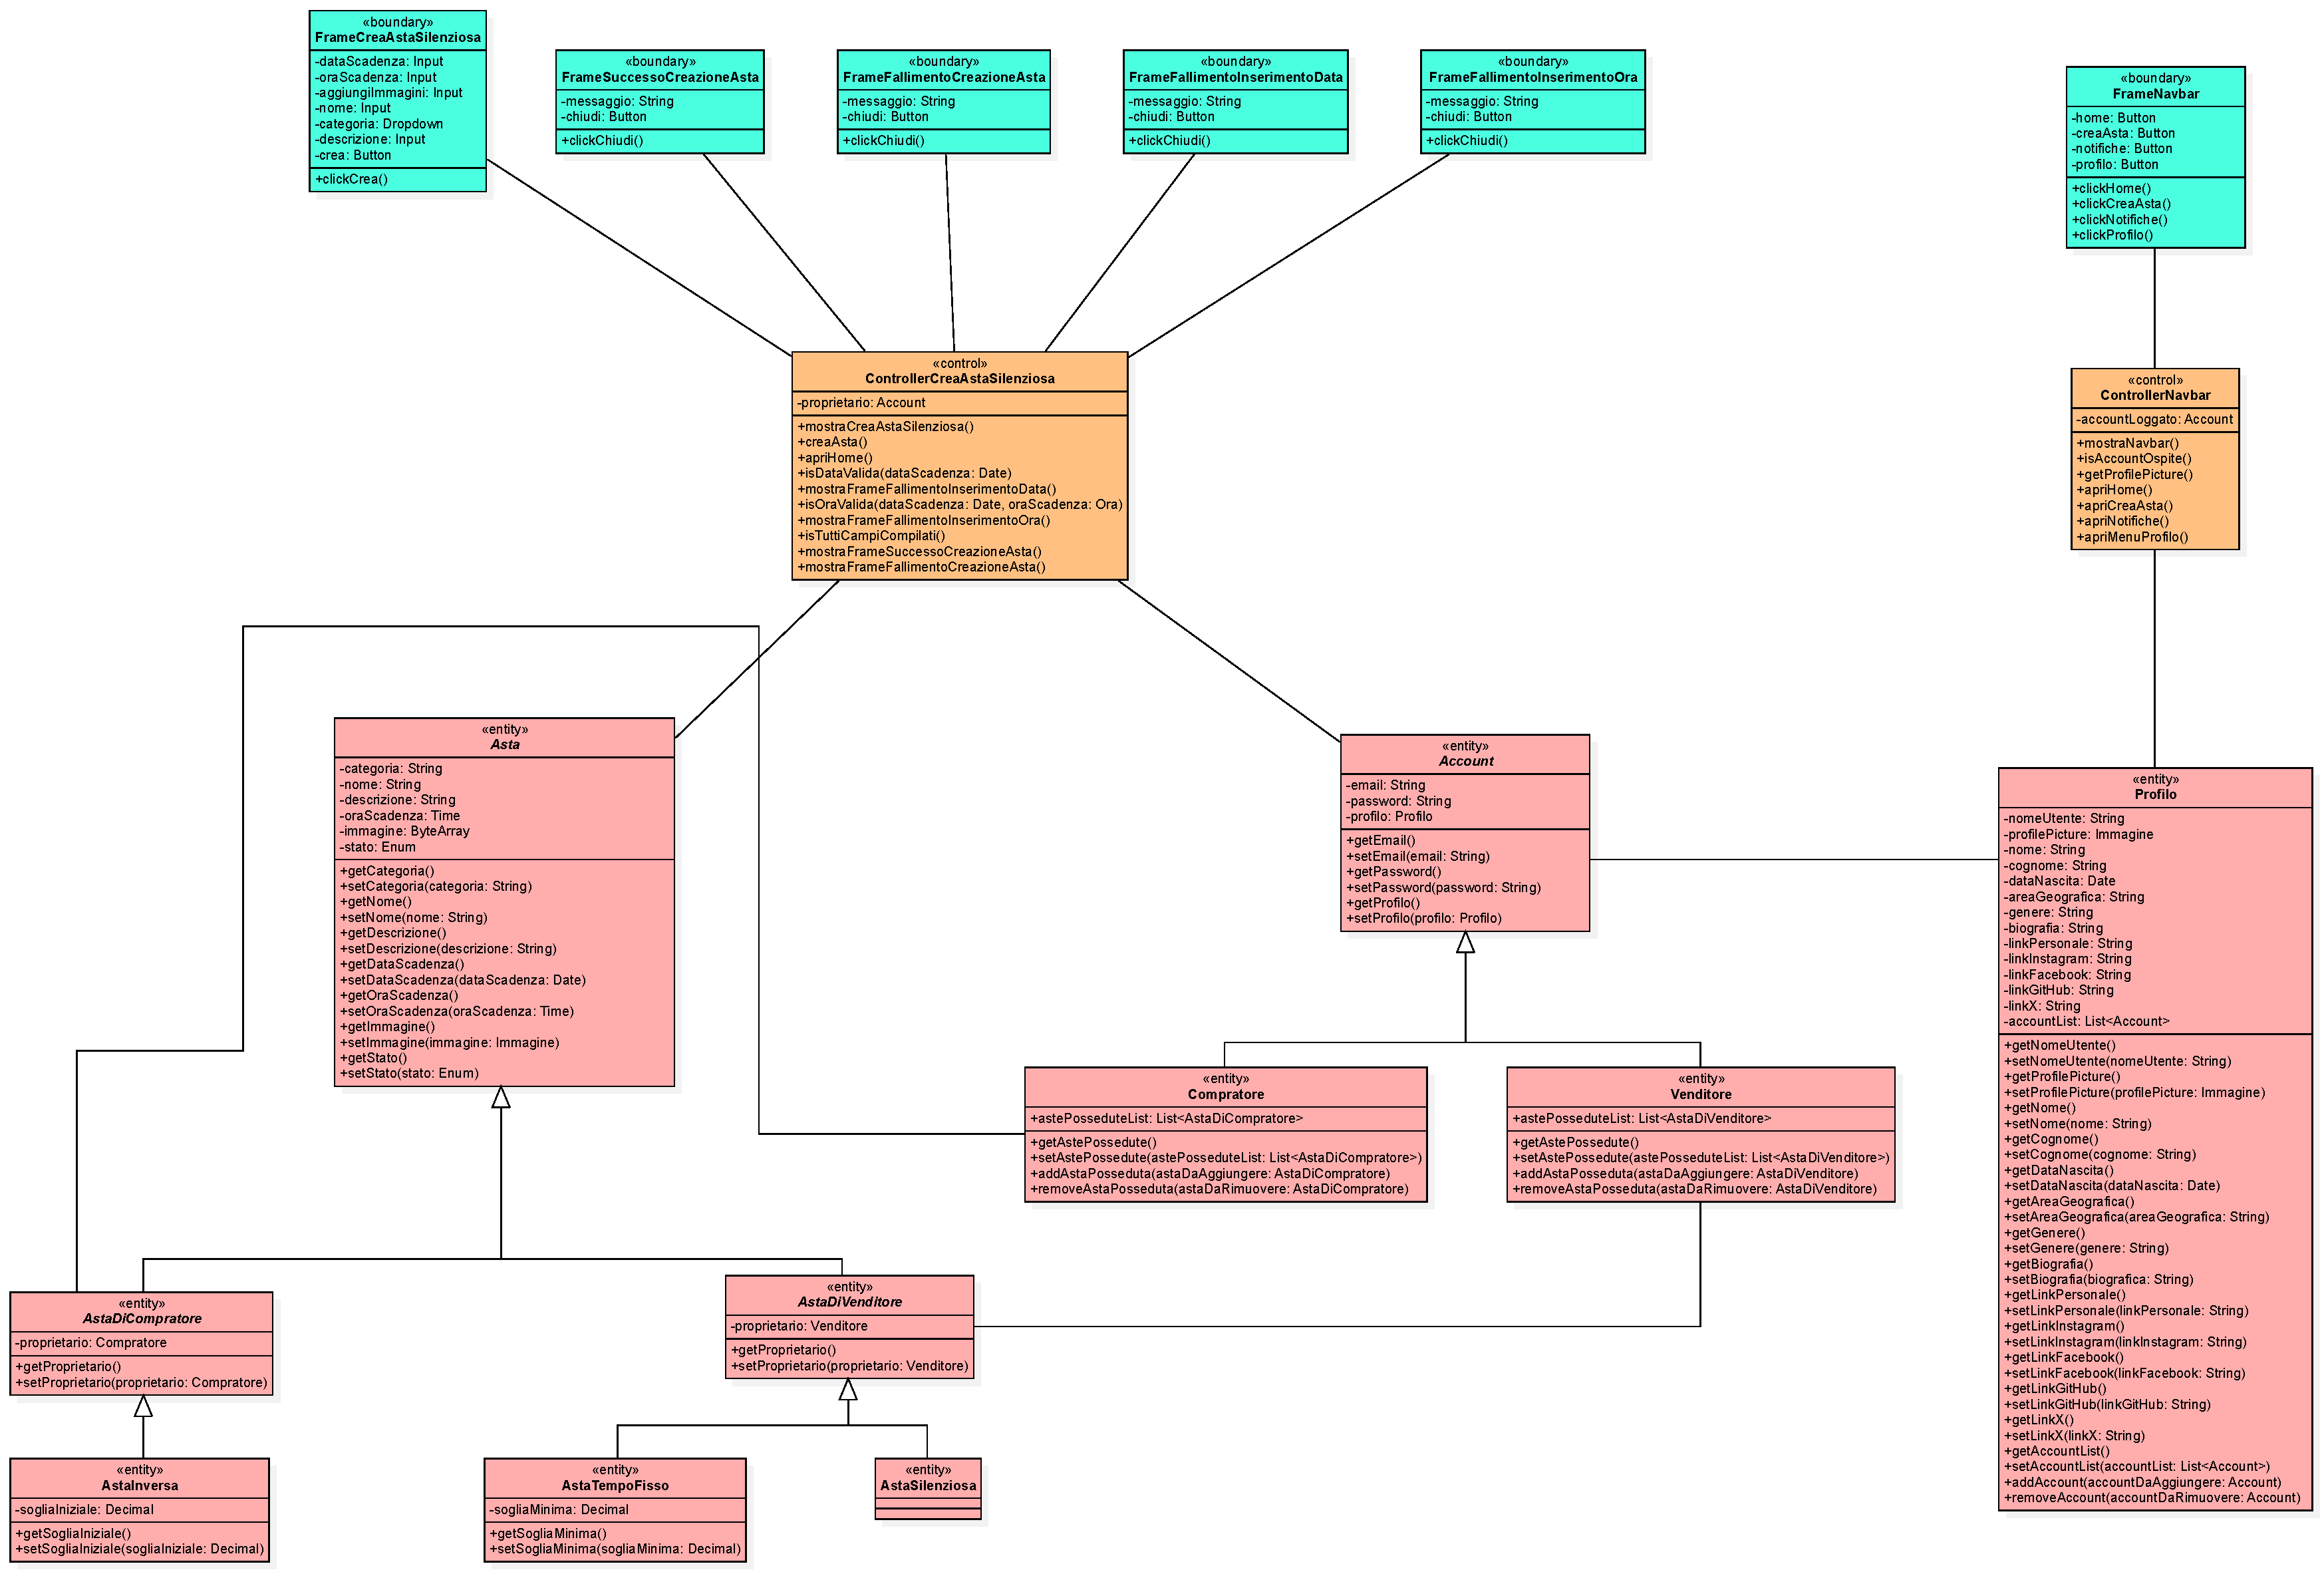
\includegraphics[width=1\linewidth]{Immagini/Diagrammi/Class Diagram/Analisi/Venditore e compratore/CreaAstaSilenziosa.pdf}
                \caption{Crea un'asta silenziosa}
            \end{figure}
            
            \begin{figure}[htbp!]
                \centering
                    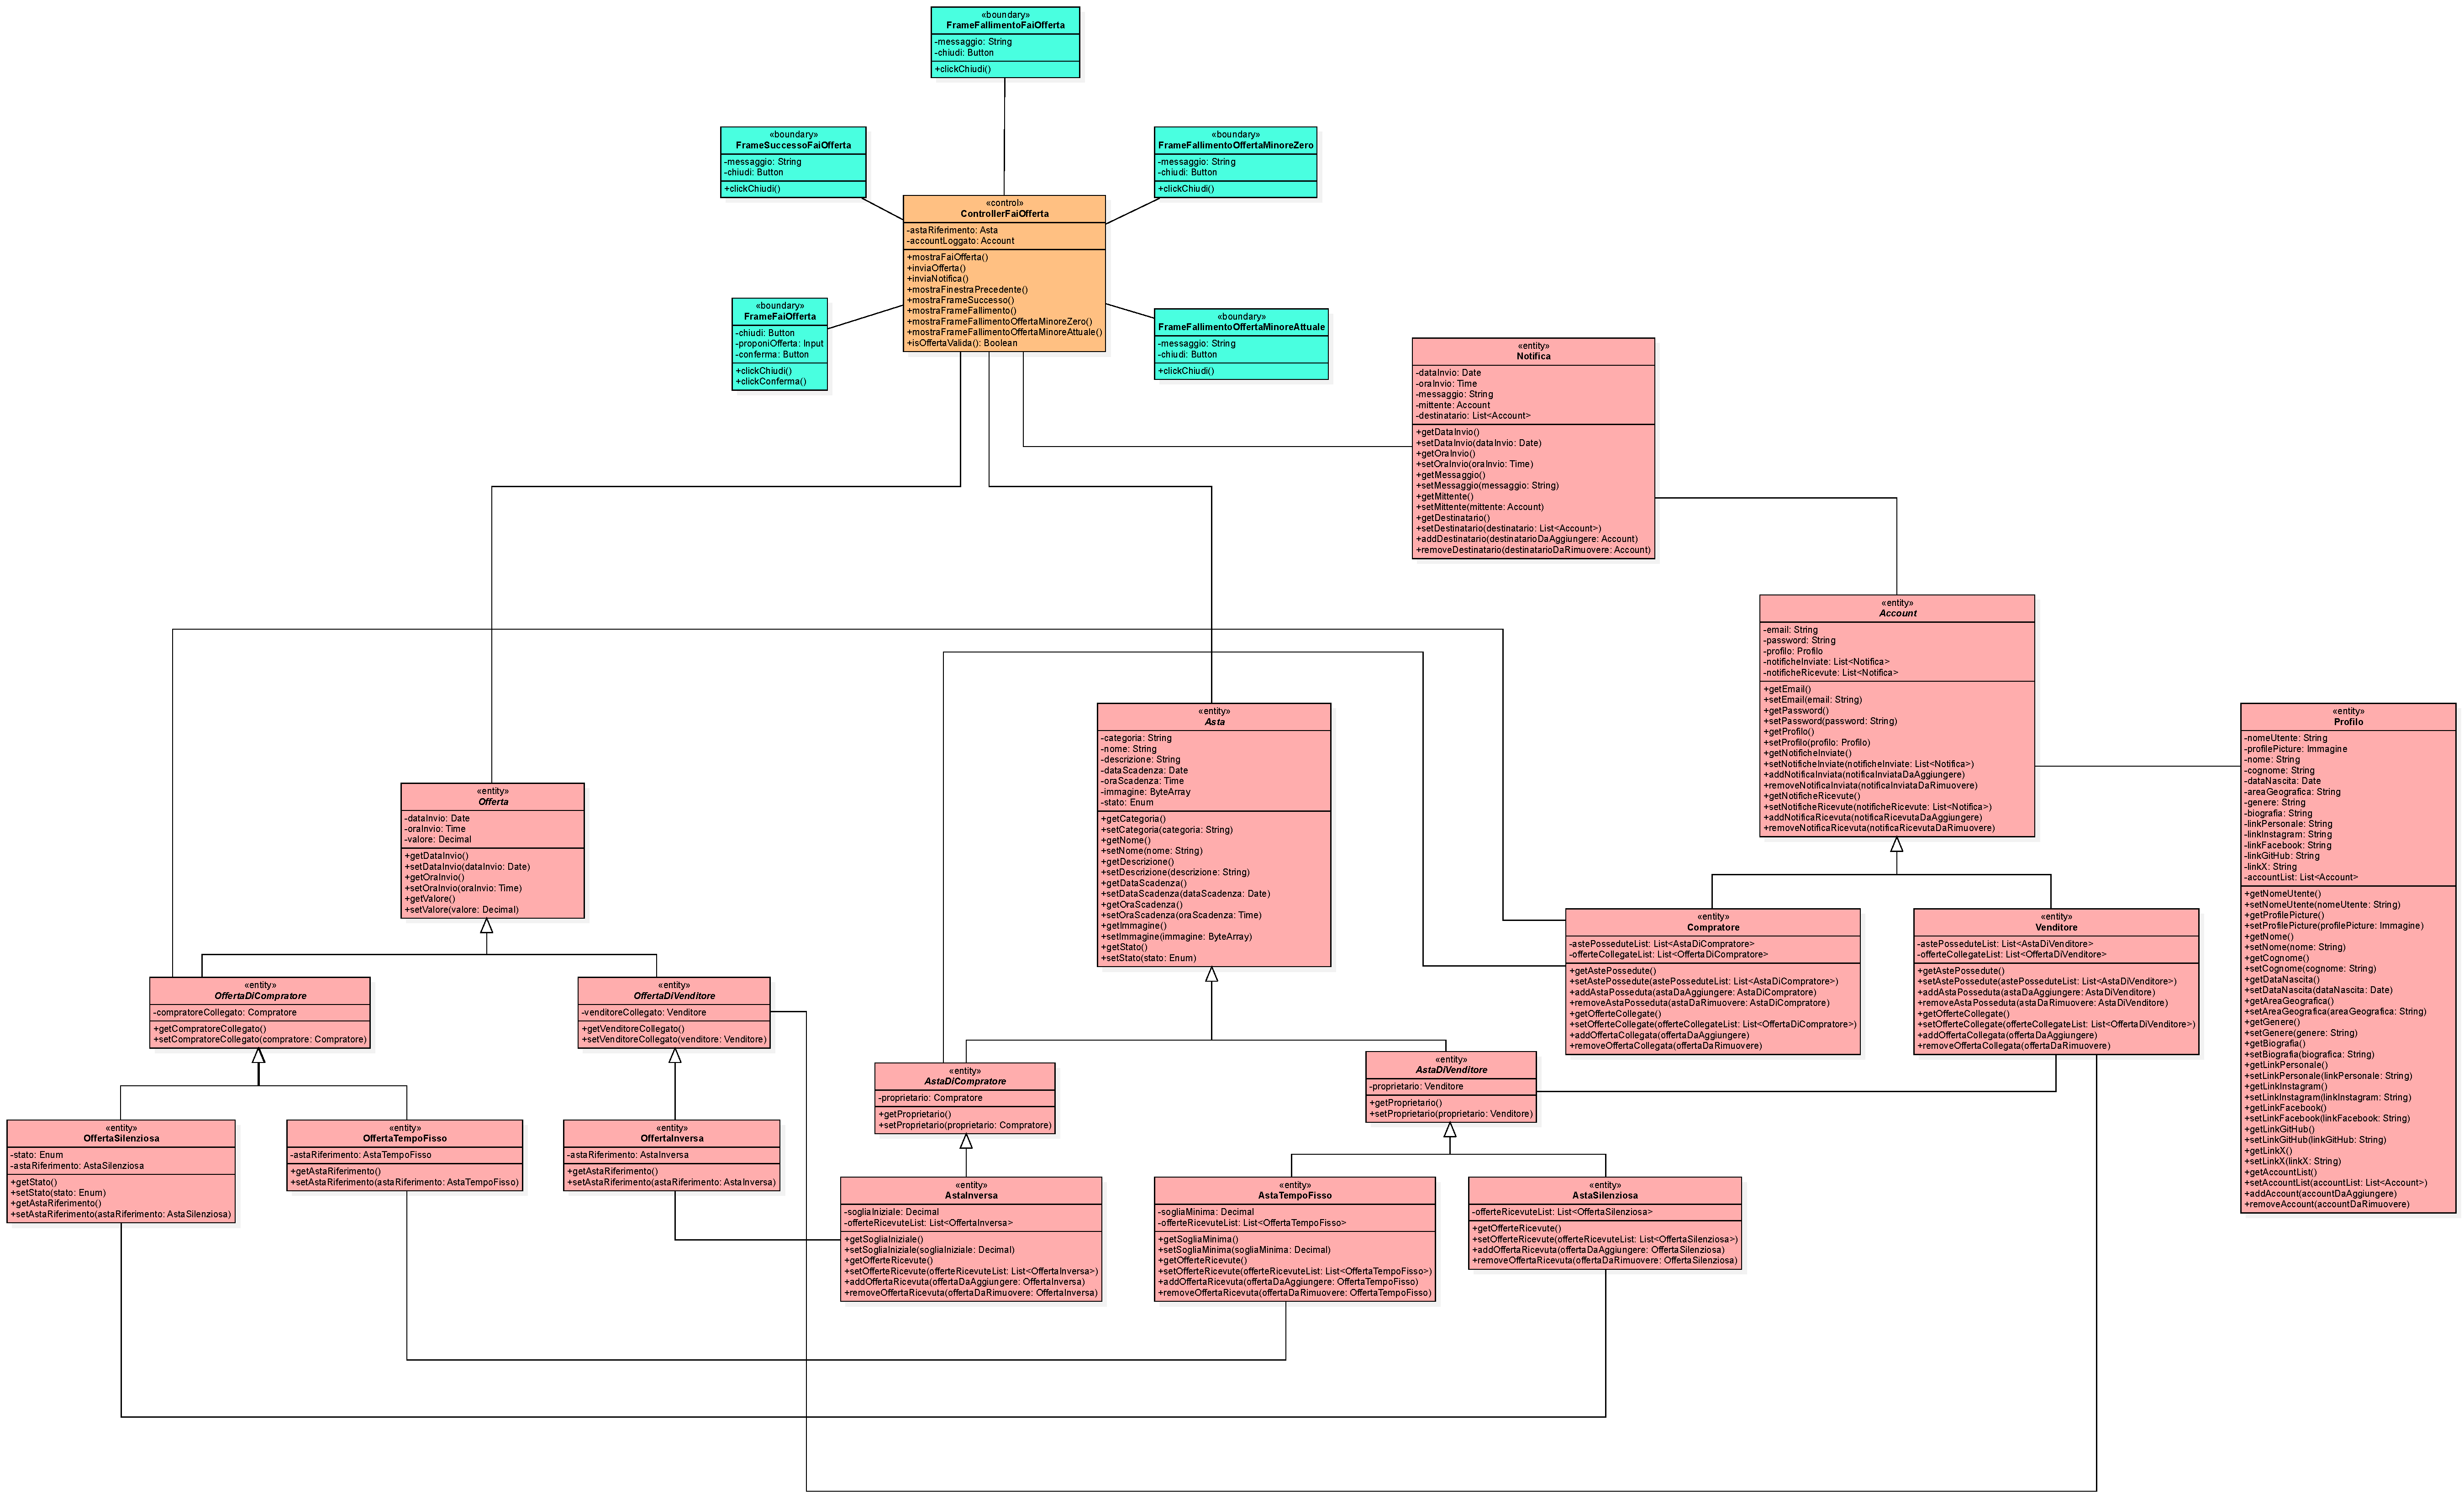
\includegraphics[width=1\linewidth]{Immagini/Diagrammi/Class Diagram/Analisi/Venditore e compratore/FaiOfferta.pdf}
                \caption{Fai un'offerta}
            \end{figure}

    \clearpage
        
    \section{Dizionario delle classi}
        \begin{longtable}{|C{3.5cm}|L{11.2cm}|}
            \hline
            \multicolumn{1}{|c|}{\cellcolor{head}\textbf{Classe}} & \multicolumn{1}{c|}{\cellcolor{head}\textbf{Descrizione}}\\  
            \hline
                Account &
                L'account raccoglie le informazioni necessarie per permettere ad un utente dell'applicazione di effettuare l'accesso alla stessa. Esso può essere di due tipologie: compratore e venditore.\\
            \hline
                Venditore &
                Un account di tipo venditore è un account che rappresenta un utente che utilizza l'applicazione per vendere i propri beni o servizi ad altri utenti.\\
            \hline
                Compratore &
                Un account di tipo compratore è un account che rappresenta un utente che utilizza l'applicazione per acquistare beni o servizi da altri utenti.\\
            \hline
                Profilo &
                Il profilo concentra le informazioni di natura personale che riguardano l'utente registrato. Esso è condiviso tra l'account compratore e venditore di uno stesso utente.\\
            \hline
                Notifica &
                Una notifica è un messaggio che viene recepito da un utente; ciò avviene quando un'asta alla quale ha partecipato si è conclusa (ed eventualmente vinta), la sua offerta è stata accettata in un'asta silenziosa, o un'asta creata ha ricevuto un'offerta da un'utente.\\
            \hline
                Asta &
                Un'asta è un annuncio di compravendita di un bene o un servizio e che raccoglie tutte le informazioni che riguardano l'articolo e chi ha pubblicato questo annuncio. Anche questa può essere di tipo compratore o venditore.\\
            \hline
                Asta di compratore &
                Un'asta di tipo compratore è un'asta nella quale il compratore richiede a dei venditori di fornirgli un bene o un servizio. Essa è di un'unica tipologia, ossia un'asta inversa.\\
            \hline
                Asta di venditore &
                Un'asta di tipo venditore è un'asta nella quale il venditore fornisce a dei compratori un bene o un servizio da essi richiesto. Essa può essere di due tipologie, ossia un'asta a tempo fisso o un'asta silenziosa.\\
            \hline
                Asta a tempo fisso &
                Un'asta a tempo fisso è un'asta nella quale si stabilisce una data di fine, entro la quale i compratori possono fare delle offerte al rialzo, e una soglia minima da raggiungere. Quando sopraggiunge la data stabilita, la persona che ha offerto la cifra più alta si aggiudica l'asta. Se non c'è stata nessuna offerta o non si è raggiunta la soglia minima entro il tempo limite, allora l'asta è dichiarata fallita.\\
            \hline
                Asta silenziosa &
                Un'asta silenziosa è un'asta nella quale si stabilisce una data di fine, entro la quale i compratori possono fare offerte al rialzo. Gli offerenti non possono però vedere l'offerta attuale più alta, e quindi dovranno offrire alla cieca. Quando sopraggiunge la data stabilita, la persona della quale l'offerta è stata accettata si aggiudica l'asta. Se non c'è stata nessuna offerta o nessuna offerta è stata accettata entro il tempo limite, allora l'asta è dichiarata fallita.\\
            \hline
                Asta inversa &
                Un'asta inversa è un'asta nella quale si stabilisce una data di fine, entro la quale i venditori possono fare offerte al ribasso, e una soglia massima da cui partire. Quando sopraggiunge la data stabilita, la persona che ha offerto la cifra più bassa si aggiudica l'asta. Se non c'è stata nessuna offerta entro il tempo limite, allora l'asta è dichiarata fallita.\\
            \hline
                Offerta &
                Un'offerta è una somma di denaro che l'utente può inviare ad un'asta con lo scopo di aggiudicarsela.\\
            \hline
                Offerta di compratore &
                Un'offerta che viene inviata da un account compratore.\\
            \hline
                Offerta di venditore &
                Un'offerta che viene inviata da un account venditore.\\
            \hline
                 Offerta a tempo fisso &
                Un'offerta che viene inviata da un account compratore ad un'asta a tempo fisso.\\
            \hline
                Offerta silenziosa &
                Un'offerta che viene inviata da un account compratore ad un'asta silenziosa.\\
            \hline
                Offerta inversa &
                Un'offerta che viene inviata da un account venditore ad un'asta inversa.\\
            \hline
        \end{longtable}
        
    \section{Dizionario delle associazioni}
        \begin{longtable}{|C{3.5cm}|L{11.2cm}|}
            \hline
                \multicolumn{1}{|c|}{\textbf{Associazione}} &
                \multicolumn{1}{c|}{\textbf{Descrizione}}\\            
            \hline
                Mittente &
                Associazione tra Account e Notifica. Quando viene inviata una notifica, essa conserva l'utente che ha effettuato l'azione che ha innescato l'invio. Una notifica ha un solo mittente, ma un mittente può essere responsabile di più notifiche.\\
            \hline
                Destinatario &
                Associazione tra Account e Notifica. Quando viene inviata una notifica, essa conserva l'utente al quale deve essere mandata per sapere a chi arrivare. Una notifica ha uno o più destinatari, e un destinatario può ricevere più notifiche.\\
            \hline
                Possiede &
                Associazione tra Account e Profilo. Quando viene creato un account, esso viene collegato ad un profilo. Un account è collegato ad un solo profilo, e un profilo è collegato al più a due account, ossia uno di tipo compratore e uno di tipo venditore.\\
            \hline
                È associata a &
                Associazione tra Notifica e Asta. Quando viene inviata una notifica, essa conserva l'asta relativa all'evento che ha causato l'invio, così che l'utente possa raggiungere velocemente l'asta attraverso la notifica. Una notifica è associata ad una sola asta, ma un'asta è associata a più notifiche.\\
            \hline
                Possiede &
                Associazione tra Venditore e Asta di venditore. Un venditore può creare un'asta per la vendita di un bene o servizio e ne diventa il possessore e gestore. Un'asta è quindi associata ad un solo venditore, ma un venditore può creare più aste.\\
            \hline
                È collegato a &
                Associazione tra Venditore e Offerta di venditore. Quando viene inviata un'offerta dal venditore, essa conserva il suo offerente così che si possa risalire ad esso nell'elenco delle offerte dell'asta. Un'offerta è collegata ad un solo venditore, ma un venditore può inviare più offerte.\\
            \hline
                Possiede &
                Associazione tra Compratore e Asta di compratore. Un compratore può creare un'asta per l'acquisto di un bene o servizio e ne diventa il possessore e gestore. Un'asta è quindi associata ad un solo compratore, ma un compratore può creare più aste.\\
            \hline
                È collegato a &
                Associazione tra Compratore e Offerta di compratore. Quando viene inviata un'offerta dal compratore, essa conserva il suo offerente così che si possa risalire ad esso nell'elenco delle offerte dell'asta. Un'offerta è collegata ad un solo compratore, ma un compratore può inviare più offerte.\\
            \hline
                Si riferisce a &
                Associazione tra Offerta a tempo fisso e Asta a tempo fisso. Ogni offerta è collegata alla relativa asta. In particolare, ogni offerta è relativa ad una sola asta e ogni asta è collegata a più offerte.\\
            \hline
                Si riferisce a &
                Associazione tra Offerta silenziosa e Asta silenziosa. Ogni offerta è collegata alla relativa asta. In particolare, ogni offerta è relativa ad una sola asta e ogni asta è collegata a più offerte.\\
            \hline
                Si riferisce a &
                Associazione tra Offerta inversa e Asta inversa. Ogni offerta è collegata alla relativa asta. In particolare, ogni offerta è relativa ad una sola asta e ogni asta è collegata a più offerte.\\
            \hline
        \end{longtable}

    \clearpage
    
    \section{Sequence Diagram}
        Il diagramma di sequenza rappresenta i processi e gli oggetti coinvolti e la sequenza dei messaggi scambiati necessari per adempiere ad una funzionalità. \\
        Le interazioni sono disposte lungo un'asse temporale per dare un'idea dell'ordine di avvicendamento dei messaggi.

        \subsection{I caso d'uso: Crea un’asta inversa}
            % Sequence Diagram costruito con StarUML
            \begin{figure}[htbp!]
            \centering
                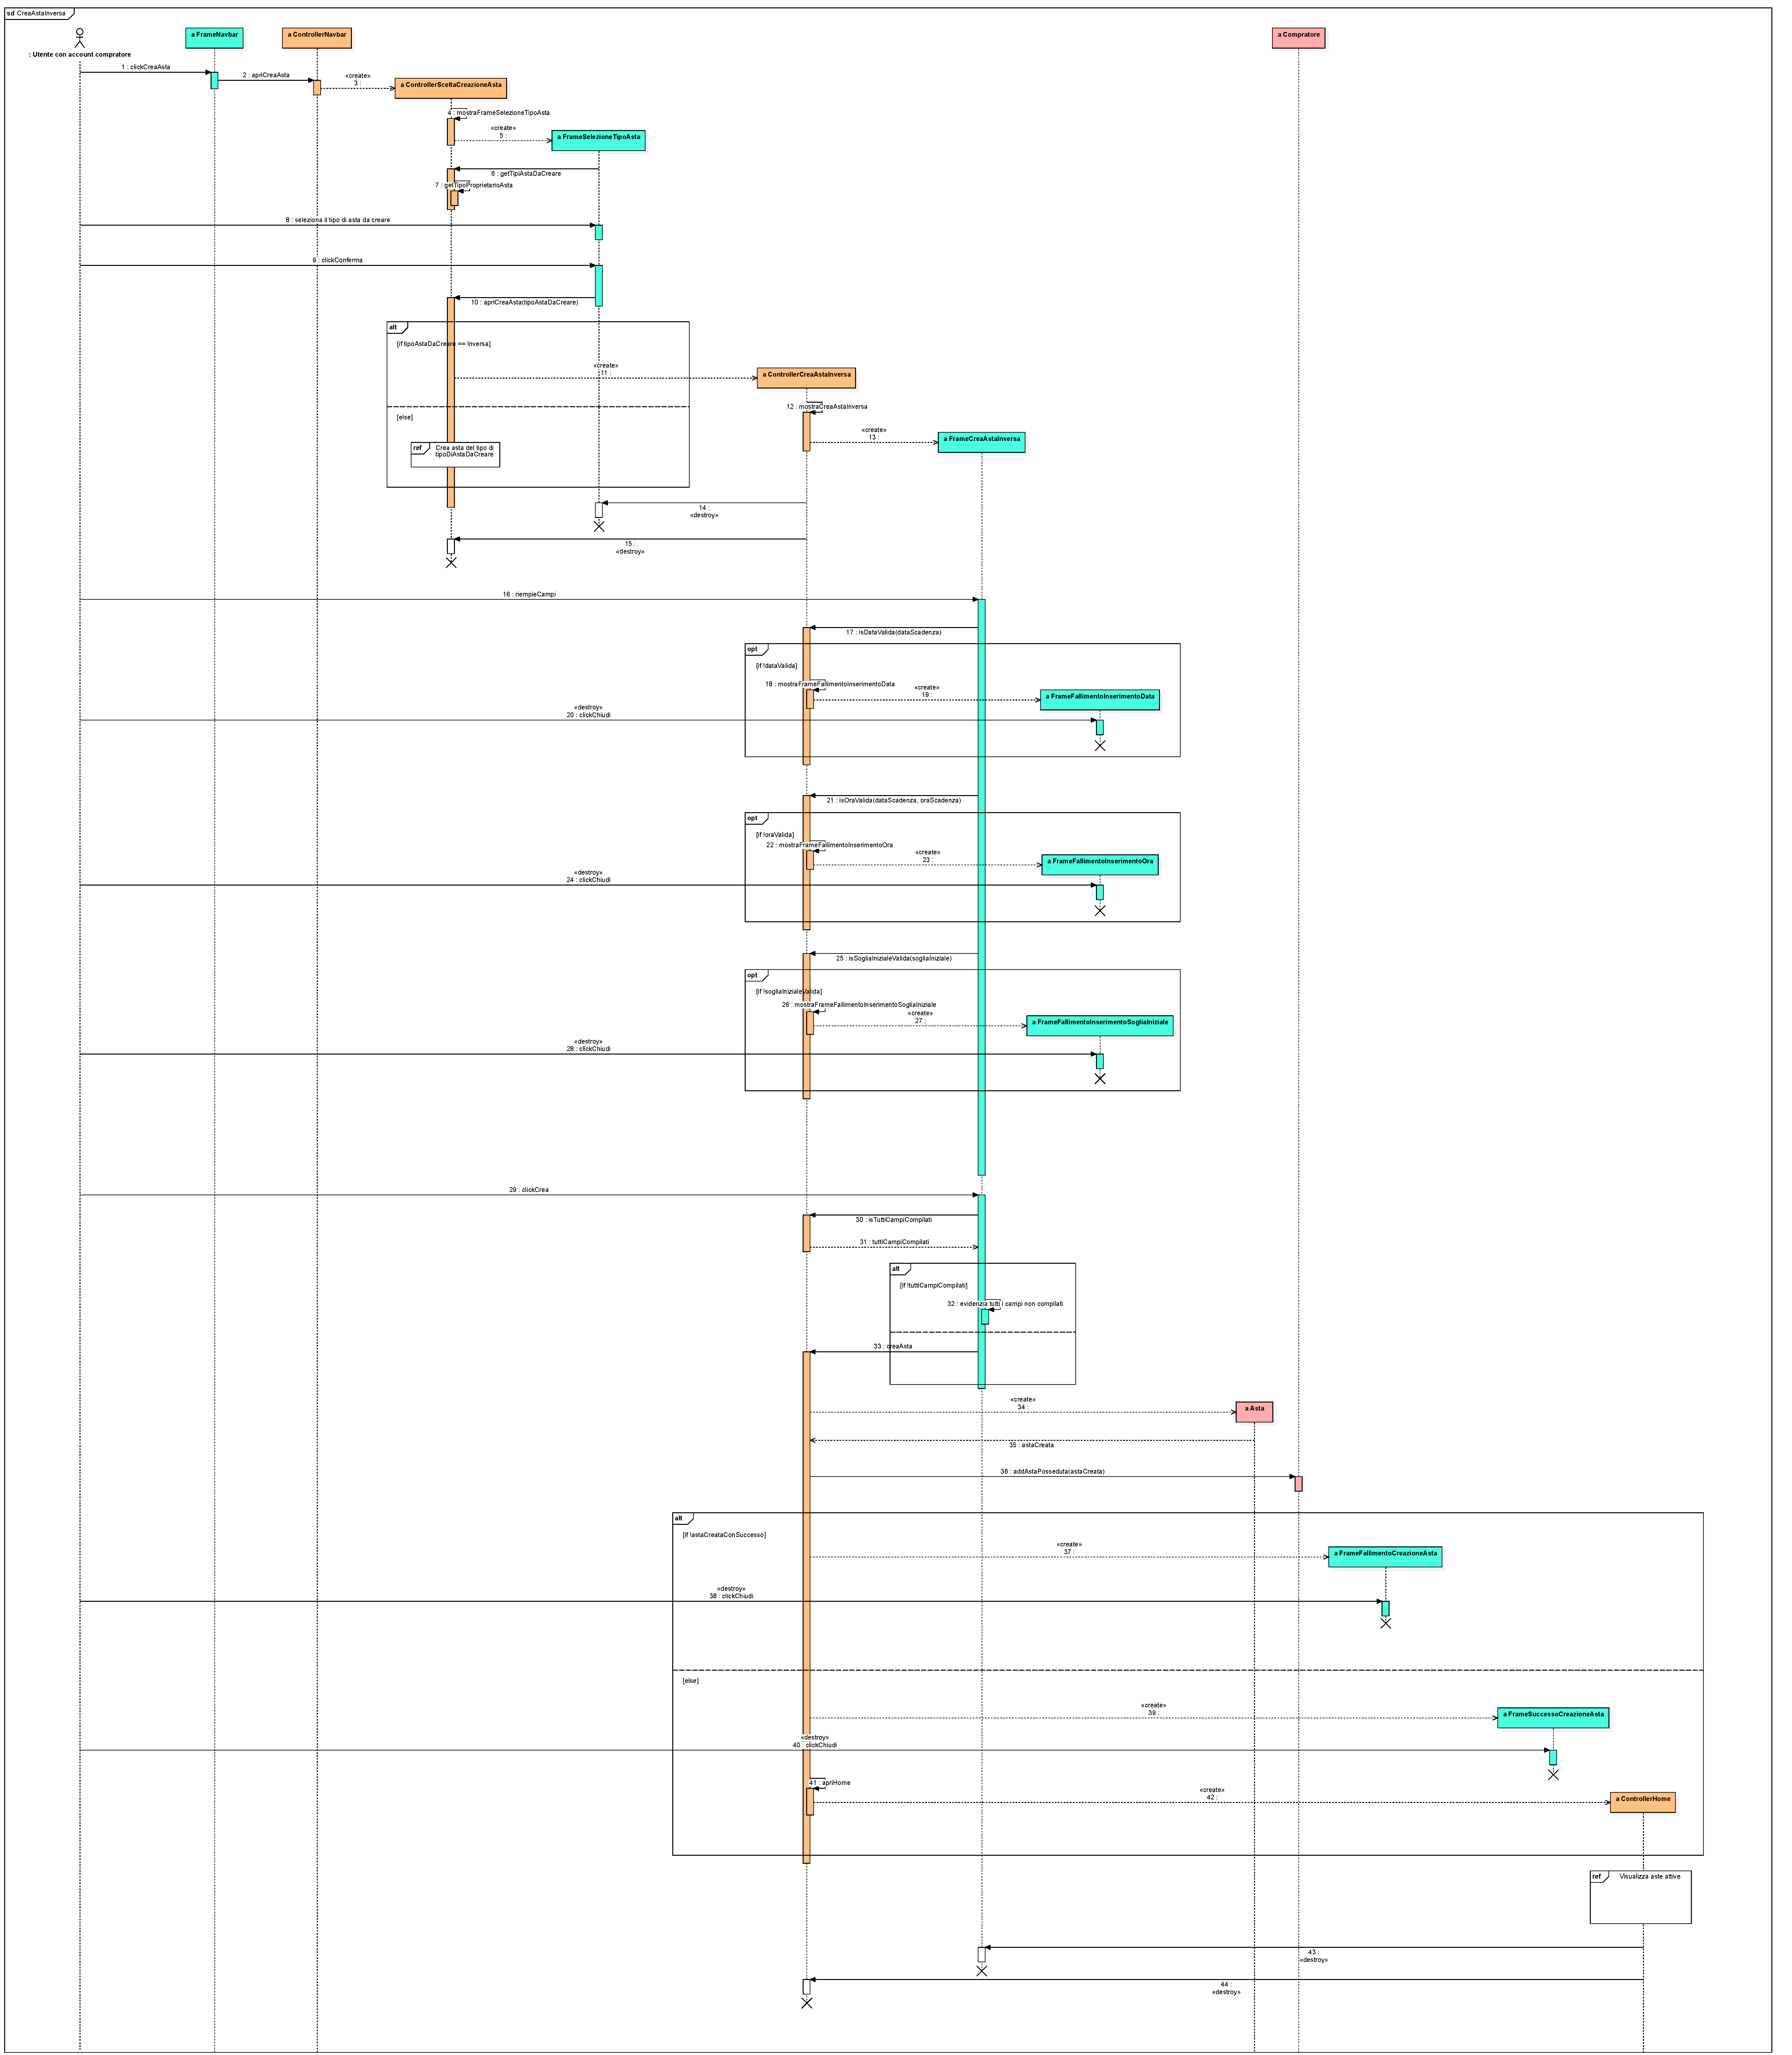
\includegraphics[width=0.93\linewidth]{Immagini/Diagrammi/Sequence Diagram/Analisi/CreaAstaInversa.pdf}
            \caption{Sequence Diagram creazione asta inversa}
            \end{figure}

        \subsection{II caso d'uso: Accetta un'offerta ricevuta all'asta silenziosa}
            % Sequence Diagram costruito con StarUML
            \begin{figure}[htbp!]
            \centering
                \includegraphics[width=1\linewidth]{Immagini/Diagrammi/Sequence Diagram/Analisi/AccettaOffertaSilenziosa.pdf}
            \caption{Sequence Diagram accetta offerta per un'asta silenziosa}
            \end{figure}

    \clearpage
    
    \section{Statechart Diagram}
        Il diagramma degli stati consente di rappresentare gli aspetti dinamici di un sistema, in particolare per l'interfaccia utente. \\
        Presenta quindi una serie di stati che il sistema attraversa (come una macchina a stati finiti), le azioni che comportano una transizione da uno stato all'altro, e le condizioni da rispettare affinché la transizione possa avvenire.

        \subsection{I caso d'uso: Crea un’asta inversa}
            % Satechart Diagram costruito con StarUML
            \begin{figure}[htbp!]
            \centering
                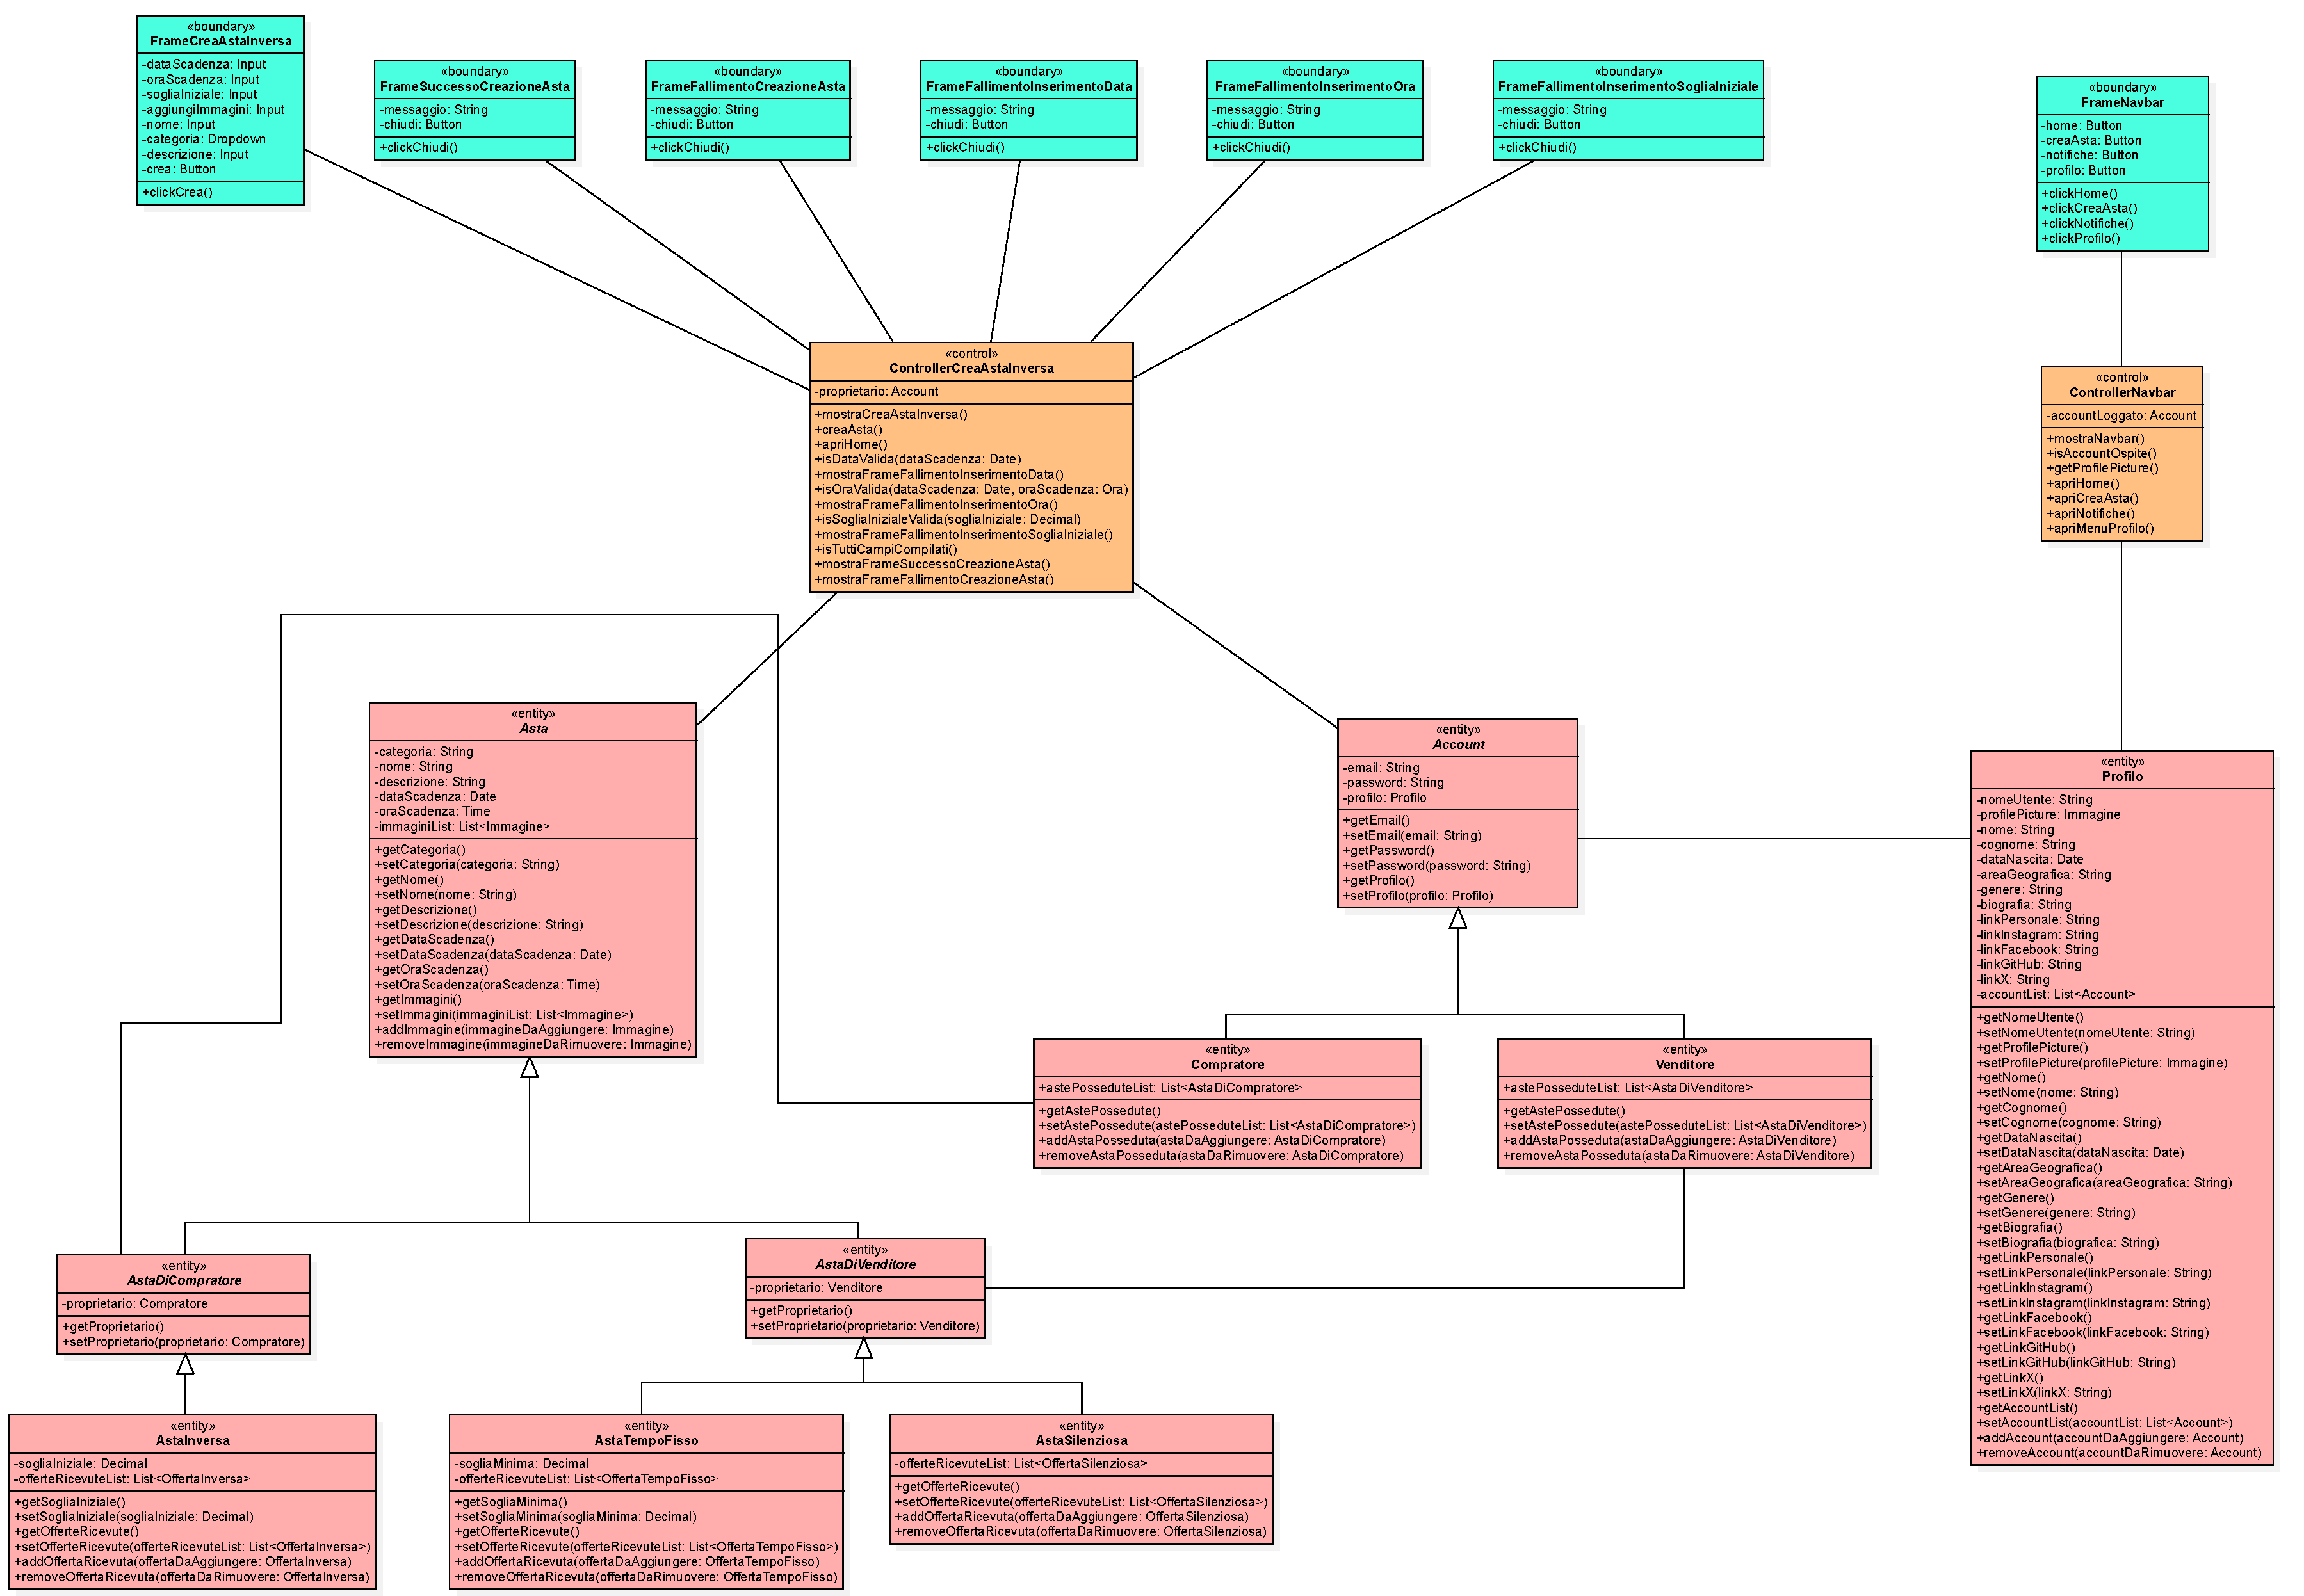
\includegraphics[width=1\linewidth]{Immagini/Diagrammi/Statechart Diagram/CreaAstaInversa.pdf}
            \caption{Statechart Diagram creazione asta inversa}
            \end{figure}

        \clearpage

        \subsection{II caso d'uso: Accetta un'offerta ricevuta all'asta silenziosa}
            % Satechart Diagram costruito con StarUML
            \begin{figure}[htbp!]
            \centering
                \includegraphics[width=1\linewidth]{Immagini/Diagrammi/Statechart Diagram/AccettaOffertaSilenziosa.pdf}
            \caption{Statechart Diagram accetta offerta per un'asta silenziosa}
            \end{figure}